\documentclass[a4paper,12pt]{report}
\usepackage{graphicx}  % For including graphics
\usepackage{hyperref}  % For hyperlinks
\usepackage{listings}  % For code snippets
\usepackage{tocbibind} % For adding ToC to the table of contents
\usepackage{titlesec}  % For customizing titles
\usepackage[ngerman]{babel}
% \usepackage{wasysym}
\usepackage{parskip}
\usepackage{bm}
\usepackage{xcolor}
\usepackage{xfrac}
\usepackage{longtable}
\usepackage{pdfpages}
\usepackage{rotating}

\lstset{
    backgroundcolor=\color{lightgray}, % Black background
    basicstyle=\ttfamily\small\color{black}, % Monospace font, white text
    frame=single, % Box around the code
    rulecolor=\color{gray}, % Border color
    breaklines=true, % Allow breaking long lines
    showstringspaces=false, % Don't show spaces as symbols
    xleftmargin=5pt, % Margin for padding
    xrightmargin=5pt,
    literate={ü}{{\"u}}1 {ö}{{\"o}}1 {ä}{{\"a}}1
}

\usepackage{geometry}
\usepackage{booktabs}
\usepackage{amsmath}
\usepackage{cleveref}

\geometry{
    top=1in,
    left=1in,
    right=1in,
    bottom=1in
}

\titleformat{\chapter}[block]   % Set chapter format to block style (both on same line)
{\normalfont\huge\bfseries}     % Format for the chapter number and title
{\thechapter}                   % Shows the chapter number followed by a dot
{0.5em}                         % Space between the chapter number and title
{}                              % Formatting for the chapter title (leave empty)

\renewcommand{\contentsname}{Inhaltsverzeichnis}
\renewcommand{\listtablename}{Tabellenverzeichnis}
\renewcommand{\listfigurename}{Abbildungsverzeichnis}
\renewcommand{\lstlistlistingname}{Code-Ausschnitte}
\renewcommand{\abstractname}{Zusammenfassung}
\renewcommand{\chaptername}{Kapitel}

\setcounter{secnumdepth}{4}

\definecolor{eclipseStrings}{RGB}{42,0.0,255}
\definecolor{eclipseKeywords}{RGB}{127,0,85}
\colorlet{numb}{magenta!60!black}

\lstdefinelanguage{json}{
    basicstyle=\normalfont\ttfamily,
    commentstyle=\color{eclipseStrings}, % style of comment
    stringstyle=\color{eclipseKeywords}, % style of strings
    numbers=left,
    numberstyle=\scriptsize,
    stepnumber=1,
    numbersep=8pt,
    showstringspaces=false,
    breaklines=true,
    frame=lines,
    backgroundcolor=\color{lightgray},
    string=[s]{"}{"},
    comment=[l]{:\ "},
    morecomment=[l]{:"},
    literate=
    *{0}{{{\color{numb}0}}}{1}
        {1}{{{\color{numb}1}}}{1}
        {2}{{{\color{numb}2}}}{1}
        {3}{{{\color{numb}3}}}{1}
        {4}{{{\color{numb}4}}}{1}
        {5}{{{\color{numb}5}}}{1}
        {6}{{{\color{numb}6}}}{1}
        {7}{{{\color{numb}7}}}{1}
        {8}{{{\color{numb}8}}}{1}
        {9}{{{\color{numb}9}}}{1}
}

\usepackage{makeidx}
\makeindex

\usepackage{glossaries}

% Define glossary entries
\newglossaryentry{acid}{
    name=ACID,
    description={Ein Akronym für Atomicity, Consistency, Isolation und Durability, Eigenschaften von Transaktionen in Datenbanksystemen}
}

\newglossaryentry{api}{
    name=API,
    description={Application Programming Interface, eine Schnittstelle zur Kommunikation zwischen Software-Komponenten}
}

\newglossaryentry{bash}{
    name=Bash,
    description={Eine Unix-Shell und Skriptsprache, häufig für Systemadministration und Automatisierung verwendet.
    In diesem Dokument für die Installation und Ausführung der Anwendung verwendet}
}

\newglossaryentry{cli}{
    name=CLI,
    description={Command Line Interface, eine textbasierte Benutzerschnittstelle zur Interaktion mit Software}
}

\newglossaryentry{crud}{
    name=CRUD,
    description={Ein Akronym für Create, Read, Update und Delete, grundlegende Operationen auf Datenbanken}
}

\newglossaryentry{csv}{
    name=CSV,
    description={Comma-Separated Values, ein Dateiformat für tabellarische Daten}
}

\newglossaryentry{cachefiles}{
    name=Cache-Dateien,
    description={Zwischengespeicherte Dateien, die häufig von Anwendungen erstellt werden, um spezifische Daten auf einem System zu speichern, damit sie schneller abgerufen werden können}
}

\newglossaryentry{dbms}{
    name=DBMS,
    description={Database Management System, Software zur Verwaltung von Datenbanken}
}

\newglossaryentry{daemon}{
    name=Daemon,
    description={Ein Hintergrundprozess, der Dienste bereitstellt oder Überwachungsaufgaben ausführt}
}

\newglossaryentry{floss}{
    name=FLOSS,
    description={Free/Libre and Open Source Software, Software, die frei verfügbar und quelloffen ist}
}

\newglossaryentry{gpt}{
    name=GPT,
    description={Generative Pre-trained Transformer, namensgebung für eine Reihe von KI-Modellen, die von OpenAI entwickelt wurden}
}

\newglossaryentry{h2}{
    name=H2,
    description={Eine leichtgewichtige, relationale Datenbank, die in-memory verwendet werden kann}
}

\newglossaryentry{http}{
    name=HTTP,
    description={Hypertext Transfer Protocol, ein Protokoll zur Übertragung von Daten im Web}
}

\newglossaryentry{jre}{
    name=JRE,
    description={Java Runtime Environment, eine Laufzeitumgebung für Java-Anwendungen}
}

\newglossaryentry{java}{
    name=Java,
    description={Die objektorientierte Programmiersprache, die in diesem Projekt verwendet wurde}
}

\newglossaryentry{kimodell}{
    name=KI-Modell,
    description={Ein Modell, das Aufgaben mithilfe von künstlicher Intelligenz löst}
}

\newglossaryentry{logfiles}{
    name=Log-Dateien,
    description={Dateien, die Ereignisse oder Nachrichten von Software dokumentieren}
}

\newglossaryentry{mit}{
    name=MIT,
    description={Eine Lizenz für freie Software, die weit verbreitet ist und die Verwendung in kommerziellen Projekten erlaubt}
}

\newglossaryentry{mvp}{
    name=MVP,
    description={Minimum Viable Product, die minimal funktionsfähige Version eines Produkts}
}

\newglossaryentry{maven}{
    name=Maven,
    description={Ein Build-Management-Tool für Java-Projekte}
}

\newglossaryentry{merkletree}{
    name=Merkle-Tree,
    description={Eine Hash-basierte Baumstruktur zur effizienten Überprüfung der Itergrität von Verzeichnissen oder Dateien}
}

\newglossaryentry{monitoring}{
    name=Monitoring,
    description={Die periodische Überwachung von Systemen oder Dateien}
}

\newglossaryentry{openai}{
    name=OpenAI,
    description={Ein Unternehmen, das KI-Modelle wie GPT entwickelt}
}

\newglossaryentry{powershell}{
    name=PowerShell,
    description={Eine plattformübergreifende Shell und Skriptsprache, entwickelt von Microsoft}
}

\newglossaryentry{prompt}{
    name=Prompt,
    description={Eine Eingabeaufforderung oder eine Frage, die einer KI gegeben wird}
}

\newglossaryentry{rest}{
    name=REST,
    description={Representational State Transfer, ein Architekturstil für Webservices (APIs)}
}

\newglossaryentry{regexpattern}{
    name=Regex-Pattern,
    description={Ein regulärer Ausdruck zur Mustererkennung in Text}
}

\newglossaryentry{sql}{
    name=SQL,
    description={Structured Query Language, eine Sprache zur Abfrage und Manipulation von Daten in relationalen Datenbanken}
}

\newglossaryentry{sqlite}{
    name=SQLite,
    description={Eine serverlose, eingebettete relationale Datenbank}
}

\newglossaryentry{shell}{
    name=Shell,
    description={Eine Schnittstelle, die die Interaktion mit dem Betriebssystem ermöglicht, oft über eine Kommandozeile}
}

\newglossaryentry{snapshot}{
    name=Snapshot,
    description={Ein Zustand eines Verzeichnisses oder einer Datei zu einem bestimmten Zeitpunkt}
}

\newglossaryentry{spring}{
    name=Spring,
    description={Ein Framework zur Entwicklung von Java-Anwendungen}
}

\newglossaryentry{token}{
    name=Token,
    description={Repräsentiert eine Einheit von Text, die von einem GPT-Modell verarbeitet wird}
}

\newglossaryentry{tracesentry}{
    name=TraceSentry,
    description={Der Name des Projekts, eine KI-gestützte Anwendung zur Überwachung von Cache- und Logdateien}
}

\newglossaryentry{ux}{
    name=UX,
    description={User Experience, das Erlebnis eines Benutzers mit einem Produkt oder einer Dienstleistung}
}


\makeglossaries

\begin{document}

% Title Page
    \begin{titlepage}
        \centering
        \textit{Berner Fachhochschule}\\[0.2em]
        \textit{BTI3031 Project 1}
        \vfill
        {\huge \textbf{TraceSentry}}\\[1em]
        {\Large AI-Aided Caches-n-Logs Monitoring-n-Wiping Daemon}\\[4em]
        {\large Luca Scherer, Janic Scherer, Luca Ammann}\\[0.5em]
        \begin{tabular}{ll}
            \textbf{Betreuer:}\hspace{0.5em}Dr. Simon Kramer \\
        \end{tabular}

        \vfill
        \textit{\today}
    \end{titlepage}

% Abstract
    \begin{abstract}
        TraceSentry ist eine plattformunabhängige und KI-gestützte Anwendung zur Suche, Über\-wachung, Bewertung und Bereinigung von Cache- und Logdateien.
        In einer praxisorientierten Fallstudie wurde das KI-Modell \textit{GPT-4o Mini} von OpenAI ausgewählt und evaluiert, um Dateiinhalte zu bewerten und potenzielle Risiken zu erkennen.
        Die Anwendung umfasst eine Befehlszeilenschnittstelle (CLI) und einen Hintergrundprozess (Daemon), der in regelmäßigen Abständen Snapshots der überwachten Verzeichnisse erstellt.
        Diese Snapshots dienen als Momentaufnahmen der Verzeichnisse, werden als Merkle-Bäume konstruiert und miteinander verglichen.
        Eine SQLite-Datenbank wird verwendet, um die Snapshots sowie die erkannten Änderungen zu persistieren.
        Die modulare Architektur der Anwendung, die in Java unter Verwendung des Spring-Frameworks implementiert wurde, ermöglicht die Erweiterung um zusätzliche Funktionen oder Benutzeroberflächen.

        Dieses Dokument beschreibt die technische Spezifikation und Umsetzung, die verwendeten Prozesse, eine umfangreiche Evaluation der Anwendung,
        die KI-Fallstudie sowie einen Ausblick auf zukünftige Arbeiten.
    \end{abstract}

% Table of Contents
    \tableofcontents
    \listoftables
    \listoffigures
    \lstlistoflistings

% Main Content


    \chapter{Einleitung}


    \section{Ausgangssituation}

    \subsection{Problem}\label{subsec:problem}
    Cache- und Logdateien\index{Cache- und Logdateien} sind temporäre Dateien, die von Betriebssystemen und
    Anwendungen zur Speicherung von Zwischenständen, Nutzeraktivitäten und
    Systemereignissen erstellt werden.
    Viele Computerbenutzer sind sich nicht bewusst, welche Arten dieser Dateien auf ihrem
    Computer existieren und insbesondere, welche Applikationen diese lesen, schreiben,
    verändern oder löschen.
    Dazu sind sich Anwender nicht bewusst, welchen Zwecken
    diese Dateien dienen und welche möglicherweise vertrauliche Informationen enthalten,
    die für Dritte von Interesse sein könnten.
    Diese Unkenntnis kann zu Datenschutzrisiken
    und fehlender Kontrolle führen.

    \subsection{Chance}\label{subsec:chance}
    Durch das Angebot an generativen KI-Modellen, die – meist frei oder relativ günstig - im
    Internet zugänglich sind, lässt sich schnell Fachkenntnis zu solchen Dateien einholen.
    Betrachtet werden hierbei vor allem die Struktur (Syntax) und Bedeutung (Semantik) von Dateiinhalten.
    Des Weiteren lassen sich Schlüsse aus Änderungen, Löschungen und Neuerstellungen von Dateien ziehen.\footnote{Evalutation durch KI-Modell in Bezug auf die Bedeutung von Änderungen, Löschungen und Neuerstellungen nicht weiter realisiert, siehe Abschnitt \nameref{sec:zukunftigearbeiten} bzw. \nameref{subsec:funktionale-erweiterungen}.}
    Durch das automatisierte Abfragen dieser KI-Modelle in einer eigenen Anwendung,
    welche unter anderem Momentaufnahmen (sogenannte\ Snapshots\index{Snapshots}) relevanter Dateipfaden und Metadaten speichert,
    sowie weitere Mehrwerte in Bezug auf die Nutzererfahrung realisiert, kann einem
    Benutzer auf einfache Art und Weise die Möglichkeit zur Kontrolle und Erleichterung dieses Umstandes
    geboten werden.

    \subsection{Antrag}\label{subsec:stakeholder}
    Das Projekt-Proposal (siehe~\nameref{sec:originale-projektbeschreibung}) umfasst einerseits die Entwicklung einer Software, welche die besagten Anforderungen erfüllt
    andererseits das Ermitteln des Potentials aktueller KI-Modelle zur Lösung des genannten Problems.\\
    Einziger Stakeholder ist Simon Kramer als Betreuer und Auftraggeber.\\


    \section{Projektziel}\label{sec:projektziel}
    Es soll eine Anwendung entwickelt werden, welche die \textbf{Suche, Überwachung und Löschung von Cache- und Logdateien\index{Cache- und Logdateien}} ermöglicht.
    Dazu gehört das \textbf{Einholen von Einschätzungen eines KI-Modells}, welches die Dateien analysiert und bewertet.
    Die Applikation soll \textbf{plattformunabhängig}, \textbf{benutzerfreundlich} und mit der nötigen \textbf{Dokumentation} für den Benutzer (User-Manual u.a.) ausgestattet sein.
    \\Das KI-Modell wird nur abgefragt bzw.\ eingebunden und dessen Entwicklung und Betrieb
    wird vom Projekt abgegrenzt.
    Passend zu dieser Abgrenzung soll als Komponente des Berichts das Potential von KI-Modellen bzw.\ des eingesetzten KI-Modells zur Lösung des Problems evaluiert werden.


    \section{Prioritäten}
    Grundsätzlich soll ein fertiges Produkt, welches dem Benutzer einen Mehrwert bietet, im Vordergrund stehen.
    Gemäss Checkliste (via Mail von Simon Kramer am 26.09.2024):
    \begin{quote}
        Resultat- statt Prozess-Orientierung priorisieren:
        \\Fertiges Projekt anstreben (Prozesse, die unfertige Resultate produzieren, vermeiden)
        \\Programme sind bessere Modelle (Spezifikations- und Design-Endlosschlaufen vermeiden)
    \end{quote}

    Priorisiert sollen dabei in erster Linie Funktionalitäten eines MVP (Minimum Viable Product) sein, welche die Kernfunktionalität des Produkts sicherstellen.
    Dazu gehören vor allem die Suche und Überwachung von Dateien.
    Zur Überwachung gehört das Erstellen von Snapshots und das Vergleichen dieser, sowie das Einholen von Einschätzungen eines KI-Modells.
    Zudem werden alle Tätigkeiten, die dabei mitschwingen, wie Dokumentation, Tests und Codequalität, als wichtig erachtet.
    Zurück priorisierte Funktionalitäten, sowie Erweiterungen werden im Kapitel~\nameref{sec:zukunftigearbeiten} beschrieben.


    \chapter{Spezifikation}\label{ch:spezifikation}


    \section{Systemabgrenzung}\label{sec:systemabgrenzung}

    \subsection{Systemumgebung (statisch)}\label{subsec:systemumgebung-(statisch)}

    \subsubsection{Systemübersicht}
    Der Hauptverwendungszweck des TraceSentry ist das Überwachen von Dateien in bestimmten Verzeichnissen.
    Dabei liegt der Fokus auf Log- und Cache-Dateien, welche periodisch auf Änderungen in Form von Erstellung, Löschung oder Veränderung überprüft werden.
    Diese periodische Überwachung soll in einem Hintergrundprozess, einem so genannten Daemon\index{Daemon}, stattfinden.
    Notwendige Daten für die Überwachung sowie, durch die Überwachung entstandene Daten, werden in einer Datenbank gespeichert.
    Verdächtige Dateien können durch eine KI-gestützte Analyse bewertet und anschliessend geleert oder gelöscht werden.

    \subsubsection{Softwarekomponenten}
    Die System- sowie Softwarearchitektur wurde im Rahmen dieser Arbeit entworfen und grundlegende Entscheide im Kapitel~\nameref{subsec:technische-variantenentscheide} festgehalten.
    Alle Softwarekomponenten wurden in Java unter der Verwendung des Spring-Frameworks entwickelt.
    Die endgültig erarbeitete Architektur wird im Kapitel~\nameref{subsec:loesungsarchitektur} beschrieben.
    Nachfolgend eine vereinfachte Übersicht der Softwarekomponenten:

    \begin{figure}[h]
        \centering
        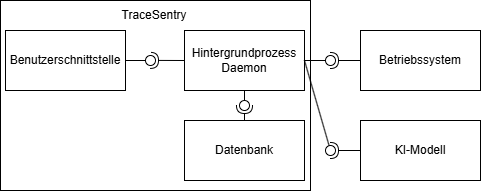
\includegraphics[width=0.6\textwidth]{assets/komponenten-grob}
        \caption{Softwarekomponenten (High-Level)}
        \label{fig:komponenten-grob}
    \end{figure}
    Die Bereitstellung und Laufzeitumgebung des Systems wird im Kapitel~\nameref{ch:bereitstellung-integration} beschrieben.

    \subsubsection{Hardwarekompatibilität}
    Der TraceSentry ist ein eigenständiges, plattformunabhängiges System, welches auf den gängigen Betriebssystemen (Windows, Linux, MacOS) lauffähig ist.
    Entwickelt und getestet wurde auf folgenden Betriebssystemen:
    \begin{itemize}
        \item Windows 11--10.0
        \item Linux 6.1.0-28
        \item macOS Sequoia 15.2
    \end{itemize}

    \subsubsection{Benutzerschnittstelle}
    Im Rahmen der Anforderungsspezifikation wurde eine Benutzerschnittstelle in Form eines Command-Line-Interfaces (CLI) spezifiziert.
    Im Hinblick auf Erweiterung und Wartbarkeit ist die Benutzerschnittstelle logisch von der Geschäftslogik getrennt.
    Aufgrund dessen wurde die Benutzerschnittstelle als eigenständige Laufzeiteinheit definiert und entwickelt.
    Die Kommunikation zwischen CLI\index{CLI} und Daemon erfolgt über eine\index{REST-API} REST-API\@.
    Diese Wahl wurde im Kapitel~\nameref{subsec:technische-variantenentscheide} begründet.

    \subsubsection{Datenbank}\label{subsubsec:spezifikation-datenbank}
    Die Datenbank wird für die Persistierung von Überwachungs-Metadaten sowie -Ergebnissen verwendet.
    Sie befindet sich lokal auf dem System in Form einer SQLite-Datenbank\index{SQLite}.
    Die Wahl des DBMS sowie dessen genaue Implementierung wird in den Kapitel~\nameref{subsubsec:technologieentscheid} und~\nameref{subsubsec:realisierung-datenbank} beschrieben.

    \subsubsection{KI-Anbindung}\label{subsubsec:spezifikation-ki-anbindung}
    Gemäss Anforderungsspezifikation wird ein KI-Modell zur Bewertung von Dateien eingebunden.
    Die Entwicklung eines eigenen KI-Modells war nicht Teil dieser Arbeit.
    Stattdessen wurde das KI-Modell \textit{GPT-4o mini} von OpenAI verwendet.
    Die Anbindung an das KI-Modell wird im Kapitel~\nameref{subsubsec:ki-anbindung} beschrieben.
    Zudem wurde eine Fallstudie zur Evaluation des Potentials eines aktuellen KI-Modells im Kontext des TraceSentry durchgeführt.
    Die Vorgehensweise sowie die Resultate dieser Fallstudie sind im Kapitel~\nameref{sec:ki-fallstudie} dokumentiert.

    \clearpage

    \subsection{Prozessumgebung (dynamisch)}\label{subsec:prozessumgebung}

    \subsubsection{Daemon Lifecycle}
    Der Daemon-Prozess\index{Daemon} kann on-demand oder als Autostart-Service gestartet werden.
    Er läuft autonom im Hintergrund und kann über die CLI angesteuert werden.

    \subsubsection{CLI Lifecycle}
    Die CLI wird on-demand pro Benutzerinteraktion gestartet und beendet.
    Das bedeutet, dass die Lebensdauer der CLI auf die Dauer einer Benutzerinteraktion beschränkt ist.
    Zusätzlich hat der Benutzer die Möglichkeit, die CLI im sogenannten \textit{interactive mode} zu starten.
    In diesem Modus steht dem Benutzer eine interaktive Shell zur Verfügung, in welcher er mehrere Befehle hintereinander ausführen kann.
    Im \textit{interactive mode} wird die CLI nicht beendet, bis der Benutzer dies explizit veranlasst.
    Dies ist ein gängiges Verhalten von Command-Line-Interfaces und ermöglicht eine effiziente Interaktion mit dem System, ohne dass für jede Benutzerinteraktion ein neuer Prozess gestartet werden muss.

    \subsubsection{Prozessübersicht}
    Nachfolgend wird davon ausgegangen, dass der Daemon-Prozess beim Systemstart gestartet wurde und sich der Benutzer im interaktiven Modus der CLI befindet.

    \paragraph*{Prozess KI-Bewertung}
    In diesem Communication Diagram wird der Prozess der, durch den Benutzer angeforderten, KI-Bewertung dargestellt.
    Die Interaktion mit dem Dateisystem ist nicht modelliert.

    Der Prozess ist für andere Funktionen des Systems identisch, weswegen auf weitere Modellierung verzichtet wird.
    Relevant für alle Prozesse ist die Kommunikation zwischen Benutzer und Daemon via CLI\@.
    Je nach Funktion interagiert der Daemon-Prozess mit dem Dateisystem, der Datenbank und dem KI-Modell.

    \begin{figure}[h]
        \centering
        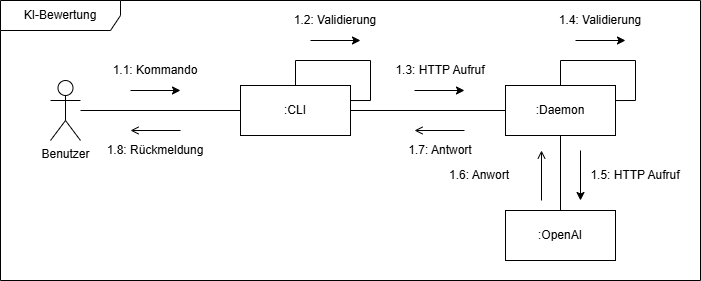
\includegraphics[width=0.8\textwidth]{assets/communication}
        \caption{Prozess KI-Bewertung (UML Communication Diagram)}
        \label{fig:communication}
    \end{figure}
    \clearpage

    \paragraph*{Prozess periodische Überwachung}
    Ein spezieller Prozess im System ist die periodische Überwachung von Dateien, da dieser autonom und ohne Benutzerinteraktion abläuft.
    Im folgenden Communication Diagram wird dieser Prozess modelliert.
    Der Daemon-Prozess ist selbständig für die Auslösung der Überwachung verantwortlich und in dieser Hinsicht nicht vom Betriebssystem abhängig.
    Die Interaktion mit dem Dateisystem ist nicht modelliert.

    \begin{figure}[h]
        \centering
        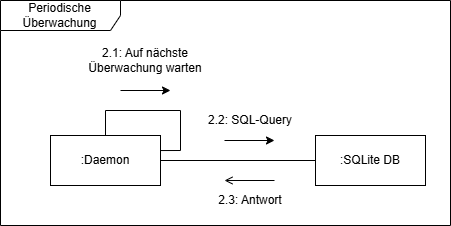
\includegraphics[width=0.8\textwidth]{assets/communication-scheduler}
        \caption{Prozess periodische Überwachung (UML Communication Diagram)}
        \label{fig:communication-scheduler}
    \end{figure}

    \subsubsection{Fehlerbehandlung}
    Wie in der Abbildung~\ref{fig:communication} ersichtlich, werden Fehler grundsätzlich auf zwei Ebenen behandelt.

    \paragraph*{CLI}
    Syntaktische oder semantische Fehler eines Kommandos werden durch die CLI behandelt.
    Die CLI gibt dem Benutzer, ohne Kommunikation mit dem Daemon, eine entsprechende Fehlermeldung zurück.

    \paragraph*{Daemon}
    Fehler, die erst während der Ausführung eines Befehls entstehen, werden durch den Daemon behandelt.
    Ein Beispiel dafür wäre eine nicht vorhandene bzw. lesbare Datei.
    In diesem Fall wird der Fehler via REST-API an die CLI zurückgegeben und dem Benutzer angezeigt.
    Fehler, die während einer periodischen Überwachung entstehen, werden geloggt und falls notwendig wird die Überwachung verworfen.

    \clearpage


    \section{Anforderungen}\label{sec:anforderungen}
    Die Anforderungen für den AI-Aided Caches-n-Logs Monitoring-n-Wiping Demon ergaben sich aus dem Projekt Proposal (siehe Anhang~\ref{sec:originale-projektbeschreibung}).
    sowie einem initialen Termin mit Herr Kramer.

    \subsection{Funktionale Anforderungen}\label{subsec:funktionale-anforderungen}

    Alle funktionalen Anforderungen werden in Form von User Stories im Scrum Product Backlog geführt.
    Dieser wird laufend erweitert beziehungsweise konkretisiert.
    Nachfolgend werden die grundlegenden Anwendungsfälle aus Benutzersicht aufgezeigt.
    \begin{figure}[h]
        \centering
        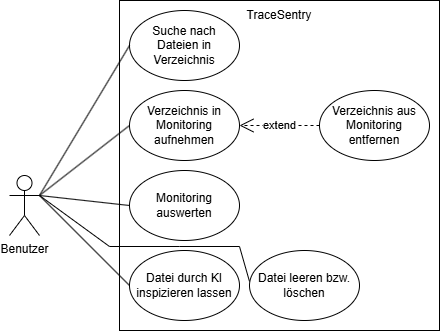
\includegraphics[width=0.6\textwidth]{assets/usecase}
        \caption{Anwendungsfälle (UML Use Case Diagram)}
        \label{fig:usecase}
    \end{figure}
    Die Anwendungsfälle wurden in folgende Hauptanforderungen an das System übersetzt,
    welche laufend konkretisiert, aufgebrochen und in User Stories inkl. Akzeptanzkriterien abgebildet wurden.
    \begin{itemize}
        \item Das System findet jegliche Dateien (insbesondere Cache- und Logdateien\index{Cache- und Logdateien} ), welche sich in einem angegebenen Verzeichnis befinden.
        (inkl. Unterverzeichnisse)
        \item Das System durchsucht periodisch angegebene Verzeichnisse inkl.
        Unterverzeichnisse nach Log- oder Cache-Dateien.
        \item Das System erstellt periodisch sogenannte Snapshots\index{Snapshots} der gefundenen Dateien, um diese später miteinander zu vergleichen.
        \item Das System identifiziert veränderte Dateien anhand der periodisch erstellten Snapshots.
        \item Das System bewertet Dateien nach deren Schädlichkeit und gibt eine Empfehlung ab, ob die Datei gelöscht oder geleert werden soll.
        \item Das System kann angegebene Dateien leeren oder löschen.
    \end{itemize}
    Auf die detaillierte Darstellung aller User Stories wird bewusst verzichtet.
    Der Einsatz von Scrum als agile Arbeitsmethode wird im Kapitel~\nameref{sec:prozesse} beschrieben.

    \newpage

    \subsection{Grenz- und Vorbedingungen}

    \subsubsection{Nichtfunktionale Anforderungen}\label{subsubsec:nichtfunktionale-anforderungen}
    Im Scrum Product Backlog werden nichtfunktionalen Anforderungen bzw.
    Grenz- oder Vorbedingungen nicht explizit als User Story geführt.
    Aus dem Projekt-Proposal und dem initialen Termin zu Projektstart ergaben sich nachfolgende nichtfunktionale Anforderungen.
    Diese beeinflussten massgeblich die Architektur des Systems.
    Keine User Story darf eine oder mehrere nichtfunktionale Anforderungen verletzten, was durch die \index{DoD} Definition of Done sichergestellt und laufend geprüft wird.

    \begin{table}[h!]
        \centering
        \setlength{\leftmargini}{0.4cm}
        \begin{tabular}{|c|p{10cm}|}
            \hline
            \textbf{ID}           & NFR-001                                                                                            \\ \hline
            \textbf{Anforderung}  & Hintergrundprozess mit periodischem Task (deamon)                                                  \\ \hline
            \textbf{Beschreibung} & Das System muss einen Hintergrundprozess implementieren, der periodisch Aktionen durchführen kann. \\ \hline
            \textbf{Akzeptanzkriterien} &
            \begin{itemize}
                \item Nach dem Start des Prozesses, ist dieser für den Benutzer nicht mehr ersichtlich.
                \item Der Hintergrundprozess ist erweiterbar, sodass dieser periodisch und autonom Aktionen durchführen kann.
            \end{itemize}
            \\ \hline
        \end{tabular}
        \caption{Nichtfunktionale Anforderung NFR-001}\label{tab:nfr-1}
    \end{table}

    \begin{table}[h!]
        \centering
        \setlength{\leftmargini}{0.4cm}
        \begin{tabular}{|c|p{10cm}|}
            \hline
            \textbf{ID}           & NFR-002                                                              \\ \hline
            \textbf{Anforderung}  & Benutzerschnittstelle via Konsole (CLI)                              \\ \hline
            \textbf{Beschreibung} & Mit dem laufenden deamon soll via Konsole interagiert werden können. \\ \hline
            \textbf{Akzeptanzkriterien} &
            \begin{itemize}
                \item Der deamon kann via CLI gestartet werden.
                \item Alle Konfigurationen und Aktionen des deamon sind via CLI verfügbar
            \end{itemize}
            \\ \hline
        \end{tabular}
        \caption{Nichtfunktionale Anforderung NFR-002}\label{tab:table4}
    \end{table}

    \begin{table}[h!]
        \centering
        \setlength{\leftmargini}{0.4cm}
        \begin{tabular}{|c|p{10cm}|}
            \hline
            \textbf{ID}           & NFR-003                                                                 \\ \hline
            \textbf{Anforderung}  & Systemunabhängigkeit                                                    \\ \hline
            \textbf{Beschreibung} & Lauffähigkeit mit vollem Funktionsumfang auf gängigen Betriebssystemen. \\ \hline
            \textbf{Akzeptanzkriterien} &
            \begin{itemize}
                \item Hintergrundprozess sowie Konsolenschnittstelle sind auf den gängigen Betriebssystemen lauffähig und mit vollem Funktionsumfang verwendbar.
                \item Alle Funktionen werden auf den Betriebssystemen Windows 11--10.0, Linux 6.1.0-28 und macOS Sequoia 15.2 getestet.
            \end{itemize}
            \\ \hline
        \end{tabular}
        \caption{Nichtfunktionale Anforderung NFR-003}\label{tab:table5}
    \end{table}
    \clearpage
    \begin{table}[h!]
        \centering
        \setlength{\leftmargini}{0.4cm}
        \begin{tabular}{|c|p{10cm}|}
            \hline
            \textbf{ID}           & NFR-004                                         \\ \hline
            \textbf{Anforderung}  & Codequalität \& erweiterbare Architektur        \\ \hline
            \textbf{Beschreibung} & Minimaler, modularer und selbsterklärender Code \\ \hline
            \textbf{Akzeptanzkriterien} &
            \begin{itemize}
                \item Die Architketur wird so aufgebaut, dass neue Features problemlos ergänzt werden können. (z.B.\ GUI)
                \item Tests gemäss Testkonzept.
                \item Statische Analysen zeigen keine schwerwiegenden verstösse gegen Linting-Regeln.
                \item Anwendungen von gängigen Design-Prinzipen vie SOLID, DRY, KISS etc.
                \item Für jede Codeerweiterung wird eine Codereview durch einen zweiten Entwickler vorgenommen.
            \end{itemize}
            \\ \hline
        \end{tabular}
        \caption{Nichtfunktionale Anforderung NFR-004}\label{tab:table6}
    \end{table}

    \subsubsection{Aktuelle Limitationen}
    Die Funktionalität des Systems ist wie folgt eingeschränkt:
    \begin{itemize}
        \item \textbf{KI-Modell}: Im Rahmen dieser Arbeit wurde nur das KI-Modell \textit{GPT-4o mini} von OpenAI integriert.
        Mit diesem lassen sich Dateien von knapp 128'000 Token bzw. rund 320'000 Zeichen analysieren.
        (siehe~\nameref{subsec:erweiterung-der-ki-modelle})
        \item \textbf{Dateigrösse}: Die maximale unterstützte Dateigrösse für die Analyse und periodische Überwachung beträgt 2GB\@.
        Diese Limitation hängt mit der Java Files API zusammen.
        (siehe~\nameref{subsec:dateikompatibilitat})
    \end{itemize}

    \subsubsection{Voraussetzungen}
    Das System wurden unter den folgenden Voraussetzungen entwickelt und getestet:
    \begin{itemize}
        \item \textbf{Java}: Es wird eine Installation der Java Runtime Environment (JRE) in Version 21 vorausgesetzt.
        \item \textbf{Dateitypen}: Das System wurde hauptsächlich mit Dateitypen getestet, die als Plaintext vorliegen, wie beispielsweise Log- oder Textdateien.
        \item \textbf{KI-Modell}: Für die Nutzung des OpenAI-Modells wird eine Internetverbindung sowie ein gültiger API-Key benötigt.
    \end{itemize}

    \clearpage

    \subsection{Testkonzept}

    \subsubsection{Ziel des Testkonzepts}
    \begin{itemize}
        \item Sicherstellen, dass das gesamte System stabil betrieben werden kann und seine Hauptfunktionen zuverlässig verfügbar sind.
        \item Minimales Testing-Setup, um den Entwicklungsaufwand gering zu halten.
        \item Fokus auf Integrationstests und funktionale Tests zur Überprüfung der gesamten Systemfunktionalität.
        \item Klare Definition, welche Tests während der Entwicklung (Teil einer User Story) umgesetzt werden sollen.
    \end{itemize}

    \subsubsection{Testarten und Testabdeckung}
    \begin{itemize}
        \item \textbf{Unit-Tests}: Auf Unit-Tests wird verzichtet und eine möglichst hohe Code-Coverage durch Integrationstests angestrebt.
        In konkreten Fällen wie Funktionen für die Such- und Überwachungsfunktionalität, können Unit-Tests für isolierte Logik implementiert werden.
        \item \textbf{Integrationstests}: Testen der Zusammenarbeit mehrerer Komponenten.
        \begin{itemize}
            \item \textbf{CLI-Befehle}: Überprüfen, dass die CLI-Kommandos (\texttt{run}, \texttt{search}) korrekt ausgeführt werden und die erwarteten Parameter validieren.
            \item \textbf{REST-HTTP-Anfragen}: Testen, ob alle HTTP-Schnittstellen korrekt reagieren.
            (Happy- sowie Exception-Paths)
        \end{itemize}
        \item \textbf{End-to-End Tests}: Fokus auf End-to-End-Szenarien zur Validierung der zentralen Funktionalität.
        (Siehe~\nameref{sec:manuelle-end-2-end-tests})
    \end{itemize}

    \subsubsection{Test-Setup und -Konfiguration}
    \begin{itemize}
        \item \textbf{Mocking von Ressourcen}: Verwenden von Mocks für Datenbank- und Dateisystemzugriffe in den Unit-Tests, um sie isoliert zu halten.
        \item \textbf{Testumgebung}: Erstellen einer dedizierten Test-DB und eines Testverzeichnisses.
        \item \textbf{Automatisierte Testausführung}: Integration der Tests in die CI/CD-Pipeline, um sicherzustellen, dass das System stabil bleibt.
    \end{itemize}

    \clearpage


    \section{Usability}\label{sec:usability}

    \subsection{Personas}\label{subsec:persona}
    Nachfolgend handelt es sich um eine fiktive Person, die als Repräsentation eines typischen Benutzers des Systems dient.

    \subsubsection{Thomas}

    Thomas ist ein 35-Jähriger Berufsschullehrer, der Informatiker und Elektroniker unterrichtet.
    Für seine Schüler unterrichtet er unter anderem auch
    Systemadministration und IT-Sicherheit.
    Thomas ist sehr interessiert an neuen Technologien und probiert gerne neue Software aus.
    Daher stellt er sich die Frage, warum so viele Log- und Cache-Dateien auf seinem Rechner sind, ob diese alle
    ihre Daseinsberechtigung haben und auch ob das Lesen und Schreiben dieser Dateien nicht ein Sicherheitsrisiko
    darstellt.
    Thomas ist ein sehr erfahrener Benutzer und hat keine Probleme mit der Kommandozeile.

    \begin{table}[h!]
        \centering
        \setlength{\leftmargini}{0.4cm}
        \begin{tabular}{|p{2.5cm}|p{7cm}|}
            \hline
            \textbf Aufgaben    & KnowHow stärken (in Bezug auf seine Lehrtätigkeiten)                      \\
            \hline
            \textbf Ziele       & Veränderungen beobachten können und diese überprüfen lassen               \\
            \hline
            \textbf Wünsche     & Intuitive Benutzerschnittstelle und teilweise Automatisierung             \\
            \hline
            \textbf Hindernisse & Trotz Erfahrung in der Informatik, sind teilweise Wissenslücken vorhanden \\
            \hline
        \end{tabular}
        \label{tab:table7}
    \end{table}

    \newpage

    \subsection{Storyboard}
    In diesem Abschnitt wird beschrieben, wie ein Nutzer mit den verschiedenen Funktionen der Software
    interagieren kann.
    Dafür ist folgend eine sinnvolle Abfolge zusammengestellt, wie ein Nutzer die Software in einem realen Anwendungsfall verwenden könnte.

    \begin{enumerate}
        \item \textbf{Dateien suchen}\\
        Der Nutzer hat kürzlich in seinem Task-Manager ein Programm entdeckt, das komischerweise
        ziemlich viel Speicher braucht.
        Also verwendet er den search-Befehl mit dem Pfad auf die Installation von diesem Programm
        und ihm werden die in diesem Verzeichnis gefundenen Cache- sowie Log-Dateien aufgelistet:
        \begin{verbatim}
internal/test.log
internal/cache.json
        \end{verbatim}

        \item \textbf{Dateien überwachen}\\
        Nun möchte der Nutzer dieses Verzeichnis \texttt{/internal} innerhalb des Programmverzeichnisses genauer überwachen.
        Also fügt er diesen Pfad mit dem monitor-Befehl hinzu und schon wird dieses Verzeichnis vom TraceSentry stündlich überwacht.

        \item \textbf{Snapshots vergleichen}\\
        Nach einigen Stunden möchte der Nutzer wissen was in diesem überwachten Verzeichnis passiert ist.
        Dafür nutzt er den snapshot compare-Befehl, um alle Zustände des Verzeichnisses vom aktuellen Zeitpunkt bis zum Start der Überwachung vergleichen zu können.
        Das System gibt ihm eine entsprechende Ausgabe:
        \begin{verbatim}
Vergleich vom Verzeichnis /internal
vom Zeitpunkt 01.12.2024 15:00:00 bis zum Zeitpunkt 01.12.2024 22:00:00:

test.log CHANGED 7-times
        \end{verbatim}

        \item \textbf{KI-Abfrage für eine Datei}\\
        Als nächstes möchte der Nutzer natürlich wissen, wofür diese test.log Datei ist, wenn sich diese jede Stunde ändert.
        Also nutzt er den inspect-Befehl, um die angebundene KI abzufragen, wofür diese Datei genau ist, ob sie ein Sicherheitsrisiko darstellt
        und ob er die Datei evtl. leeren oder sogar löschen kann.
        Daraus kommt dann eine standardisierte Ausgabe von der KI:
        \begin{verbatim}
Die Datei ist unbekannt für dieses Programm und deswegen potenziell
schädlich, also empfehle ich es zu leeren.
        \end{verbatim}

        \item \textbf{Datei leeren oder löschen}\\
        Zum Schluss kann der Nutzer dann selbst entscheiden was er mit dieser Information anfangen möchte.
        In diesem Fall möchte er dem Ratschlag der KI folgen und die Datei leeren.
        Also nutzt er den wipe-Befehl mit dem Pfad der test.log Datei und das System leert die Datei wie gewünscht.
    \end{enumerate}

    \newpage

    \subsection{UX-Prototyping}
    Da das System ausschließlich über ein Command-Line-Interface (CLI) verfügt,
    wird die Dokumentation dieser Schnittstelle im nachfolgenden Kapitel \hyperref[sec:user-manual]{Benutzerhandbuch}
    umfassend behandelt.
    Diese Dokumentation wurde im Rahmen eines iterativen und agilen Entwicklungsprozesses
    kontinuierlich während der Implementierung der einzelnen Befehle erstellt.
    Sie enthält eine detaillierte Beschreibung aller verfügbaren Befehle, einschließlich ihrer Syntax, Parameter und Anwendungsbeispiele.
    Darüber hinaus werden mögliche Systemantworten im Kontext verschiedener Szenarien erläutert,
    um eine praxisnahe Nutzung zu gewährleisten.


    \chapter{Implementierung}


    \section{Architektur}

    \subsection{Technische Variantenentscheide}\label{subsec:technische-variantenentscheide}

    \subsubsection{Architekturentscheid}
    In diesem Abschnitt werden die Überlegungen zur Architektur des Systems dargestellt.
    Es wird erläutert, welche Varianten in Betracht gezogen wurden, welche Entscheidung getroffen wurde und welche Gründe dazu geführt haben.

    \paragraph*{1. Datenbank}\mbox{}\\
    Eine zentrale Anforderung besteht darin, dass Pfad-Analysen zu einem späteren Zeitpunkt miteinander verglichen werden können.
    Daraus ergibt sich die Notwendigkeit, eine Datenbank (DBMS) zu integrieren.
    Im Folgenden werden die in Betracht gezogenen Varianten analysiert.

    \paragraph*{1.1 In-Memory}\mbox{}\\
    Bei dieser Variante wird die Datenbank während der Laufzeit des Programms im Arbeitsspeicher initialisiert und beim Beenden des Programms wieder gelöscht.
    Dies bedeutet, dass die Datenbank nur temporär verfügbar ist und den Hauptspeicher des Systems nutzt.

    \paragraph*{Vorteile}
    \begin{itemize}
        \item Sehr hohe Zugriffsgeschwindigkeit, da die Daten im Arbeitsspeicher gehalten werden.
        \item Einfache Integration ohne dauerhaften Speicherbedarf.
    \end{itemize}

    \paragraph*{Nachteile}
    \begin{itemize}
        \item Keine Persistenz der Daten über die Laufzeit hinaus.
        \item Erhöhter Speicherbedarf während der Laufzeit des Programms.
    \end{itemize}

    \paragraph*{Fazit}
    Diese Variante wurde ausgeschlossen, da die Persistenz der Daten eine essentielle Anforderung darstellt.
    Eine In-Memory-Datenbank würde nicht ermöglichen, dass Analysen auch nach einem Neustart des Systems verfügbar bleiben.

    \paragraph*{1.2 Remote}\mbox{}\\
    Bei dieser Variante wird die Datenbank auf einem externen System betrieben und über das Netzwerk vom Abnehmer aus angesprochen.
    Die Daten bleiben persistent, solange sie auf dem externen System nicht gelöscht werden und dieses ordnungsgemäß funktioniert.

    \paragraph*{Vorteile}
    \begin{itemize}
        \item Höhere Datensicherheit, da die Daten auf einem separaten System gespeichert werden können, welches durch Backup-Strategien abgesichert ist.
        \item Größere Speicherkapazität, da die Skalierung auf leistungsfähige Server oder Cloud-Dienste möglich ist.
    \end{itemize}

    \paragraph*{Nachteile}
    \begin{itemize}
        \item Abhängigkeit von einer stabilen Netzwerkverbindung, wodurch das System ohne Internet nicht verfügbar ist.
        \item Zusätzlicher Aufwand und Kosten durch die Einrichtung und Wartung der externen Infrastruktur.
    \end{itemize}

    \paragraph*{Fazit}
    Die Remote-Datenbank wurde als ungeeignet für diesen Anwendungsfall bewertet.
    Die Vorteile wie erhöhte Datensicherheit und Skalierbarkeit sind für das derzeitige System nicht notwendig, da es sich um eine kleine, lokal betriebene Anwendung handelt.
    Die zusätzlichen Anforderungen an Infrastruktur und die Abhängigkeit von einer Netzwerkverbindung stellen einen unverhältnismäßigen Mehraufwand dar, der den Nutzen nicht rechtfertigt.

    \paragraph*{\underline{1.3 Eingebettet}}\mbox{}\\
    Eine eingebettete Datenbank wird als Ressource des Programms bereitgestellt und bleibt persistent, solange die entsprechenden Dateien im Programmverzeichnis nicht gelöscht werden.
    Sie bietet eine leichtgewichtige Lösung für kleinere Anwendungen.

    \paragraph*{Vorteile}
    \begin{itemize}
        \item Keine Notwendigkeit für externe Infrastruktur, wodurch die Einrichtung vereinfacht wird.
        \item Volle Offline-Funktionalität, da keine Verbindung zu externen Diensten erforderlich ist.
        \item Hohe Performance durch direkte Anbindung an das Programm.
    \end{itemize}

    \paragraph*{Nachteile}
    \begin{itemize}
        \item Risiko eines Datenverlusts bei Fehlern oder Ausfällen des Anwendersystems.
        \item Eingeschränkte Skalierbarkeit bei wachsenden Datenmengen.
    \end{itemize}

    \paragraph*{Fazit}
    Die eingebettete Datenbank wurde als die am besten geeignete Option identifiziert.
    Sie erfüllt die Anforderungen eines kleinen Systems ohne die Notwendigkeit zusätzlicher Infrastruktur und ermöglicht eine einfache und schnelle Einrichtung.
    Da das System hauptsächlich offline betrieben werden soll, bietet diese Lösung eine optimale Balance zwischen Effizienz und Funktionalität.
    Die Verantwortung für die Datenbank wird dabei auf den Anwender übertragen, was den Verwaltungsaufwand reduziert.

    \paragraph*{2. Schnittstelle CLI $\leftrightarrow$ Daemon}\mbox{}\\
    Für die Kommunikation zwischen der CLI (Command Line Interface) und dem Daemon ist eine geeignete Schnittstelle erforderlich, um Anweisungen des Anwenders effizient und zuverlässig zu übertragen.
    Im Folgenden werden die in Betracht gezogenen Varianten analysiert.

    \paragraph*{2.1 Inter-Prozess-Kommunikation (IPC)}\mbox{}\\
    Diese Variante nutzt einen gemeinsamen Speicherbereich, beispielsweise ein geteiltes Verzeichnis, um Dateien für die Kommunikation zwischen CLI und Daemon auszutauschen.
    Die CLI schreibt Anweisungen in Dateien, die der Daemon anschließend ausliest und verarbeitet.

    \paragraph*{Vorteile}
    \begin{itemize}
        \item Einfach zu implementieren bei lokalem Einsatz auf demselben Rechner.
        \item Keine Netzwerkkonfiguration erforderlich.
    \end{itemize}

    \paragraph*{Nachteile}
    \begin{itemize}
        \item Erfordert die Definition eines eigenen Dateiformats und entsprechender Parser.
        \item CLI und Daemon müssen auf demselben System laufen, was die Flexibilität einschränkt.
        \item Es besteht das Risiko von Konflikten beim gleichzeitigen Schreiben und Lesen von Dateien, was zusätzliche Synchronisationsmechanismen erfordert.
    \end{itemize}

    \paragraph*{Fazit}
    Diese Option wurde aufgrund ihrer mangelnden Flexibilität und Erweiterbarkeit ausgeschlossen.
    Insbesondere die lokale Bindung zwischen CLI und Daemon sowie die fehlende Standardisierung und Robustheit der Kommunikation sprechen gegen diese Variante.
    Für zukünftige Anforderungen, wie die Kommunikation über ein Netzwerk, wäre sie ungeeignet.

    \paragraph*{2.2 Netzwerk-Sockets}\mbox{}\\
    Netzwerk-Sockets ermöglichen die Kommunikation zwischen Prozessen durch das Senden und Empfangen binärer Daten über spezifische Ports.
    Diese Methode kann sowohl lokal als auch über das Netzwerk verwendet werden.

    \paragraph*{Vorteile}
    \begin{itemize}
        \item Einfach zu verwenden und flexibel steuerbar.
        \item Unterstützt die Kommunikation zwischen CLI und Daemon auf getrennten Systemen über das Netzwerk.
        \item In Java durch das \texttt{java.net}-Package nativ verfügbar.
    \end{itemize}

    \paragraph*{Nachteile}
    \begin{itemize}
        \item Nachrichtenformat muss individuell definiert und implementiert werden, was zusätzlichen Entwicklungsaufwand verursacht.
    \end{itemize}

    \paragraph*{Fazit}
    Obwohl Netzwerk-Sockets eine flexible und leistungsfähige Lösung darstellen, wurde diese Variante zugunsten der REST-Schnittstelle verworfen.
    Die REST-Implementierung erscheint aufgrund ihrer Standardisierung und einfacher Handhabung im Kontext des Projekts effizienter.
    Zudem entfällt der Aufwand für die Definition und das Parsen eines eigenen Nachrichtenformats.

    \paragraph*{\underline{2.3 REST-Schnittstelle}}\mbox{}\\
    Die REST-Schnittstelle ermöglicht den Austausch von Ressourcen zwischen Client und Server über das HTTP-Protokoll.
    Der Austausch erfolgt im Rahmen definierter Formate (Content-Types) und kann über das Netzwerk abgewickelt werden.

    \paragraph*{Vorteile}
    \begin{itemize}
        \item Standardisierte Schnittstelle, die durch zahlreiche Frameworks unterstützt wird.
        \item Hohe Robustheit, da REST auf etablierten HTTP-Standards basiert.
        \item Ermöglicht die Ausführung von CLI und Daemon auf getrennten Systemen, was eine flexible Architektur fördert.
    \end{itemize}

    \paragraph*{Nachteile}
    \begin{itemize}
        \item Erfordert die Implementierung eines Webservices, was zusätzlichen Entwicklungsaufwand bedeutet.
    \end{itemize}

    \paragraph*{Fazit}
    Die REST-Schnittstelle wurde als die bevorzugte Option gewählt, da sie eine klare und standardisierte technische Kommunikation ermöglicht.
    Sie ist stabil, flexibel und erweiterbar, was besonders wichtig für den langfristigen Betrieb und mögliche zukünftige Anforderungen, wie die Systemtrennung von CLI und Daemon, ist.
    Zudem ist die Implementierung dank vorhandener Frameworks verhältnismäßig einfach und effizient.
    \clearpage

    \subsubsection{Technologieentscheid}\label{subsubsec:technologieentscheid}
    In diesem Abschnitt werden die Überlegungen zu den Technologien für die verschiedenen Systemkomponenten dargestellt.
    Basierend auf einer Analyse der Vor- und Nachteile wurde eine Entscheidung für die geeignetsten Technologien getroffen.

    \paragraph*{1. Datenbank}\mbox{}\\
    Die Auswahl einer passenden Datenbank ist entscheidend für die Persistenz und Verarbeitung der Anwendungsdaten.
    Dabei wurde zunächst die grundsätzliche Entscheidung zwischen \textbf{NoSQL} und \textbf{SQL} analysiert.

    \paragraph*{1.1 NoSQL}\mbox{}\\
    NoSQL-Datenbanken verwenden flexible Datenmodelle wie Dokumente, Key-Value oder Graphen und sind für hohe Skalierbarkeit sowie große Datenmengen ausgelegt.

    \paragraph*{Vorteile}
    \begin{itemize}
        \item Hohe Flexibilität: Anpassbare Datenstrukturen ohne festes Schema.
        \item Einfache horizontale Skalierbarkeit: Gut geeignet für große Datenmengen.
        \item Spezialisierung: Verschiedene Modelle für spezifische Anwendungsfälle.
    \end{itemize}

    \paragraph*{Nachteile}
    \begin{itemize}
        \item Fehlende Standardisierung: Unterschiedliche Abfragesprachen und Protokolle je nach Implementierung.
        \item Eingeschränkte Transaktionssicherheit: ACID-Eigenschaften werden häufig zugunsten der Performance vernachlässigt.
        \item Höhere Komplexität: Abfragen sind weniger intuitiv als in SQL-basierten Systemen.
    \end{itemize}

    \paragraph*{Fazit}
    Die Vorteile von NoSQL-Datenbanken bringen für dieses Projekt keinen nennenswerten Mehrwert, da dieser Anwendungsfall keine besonderen Anforderungen an Skalierbarkeit oder unstrukturierte Daten stellt.
    Auch aufgrund mangelnder Erfahrung im Team mit NoSQL-Systemen wurde diese Option verworfen.

    \paragraph*{\underline{1.2 SQL}}\mbox{}\\
    SQL-Datenbanken basieren auf einem relationalen Modell mit festen Schemata.\index{SQLite}
    Sie verwenden die standardisierte Abfragesprache SQL und sind besonders geeignet für datenintensive Anwendungen mit hohen Anforderungen an Konsistenz.

    \paragraph*{Vorteile}
    \begin{itemize}
        \item Standardisierung: Einheitliche Abfragesprache und breite Unterstützung.
        \item Datenkonsistenz: Verlässliche Transaktionen dank ACID-Eigenschaften.
        \item Leistungsstarke Abfragemöglichkeiten: Geeignet für komplexe relationale Analysen.
    \end{itemize}

    \paragraph*{Nachteile}
    \begin{itemize}
        \item Feste Schemata: Weniger flexibel bei Änderungen in der Datenstruktur.
        \item Begrenzte horizontale Skalierbarkeit: Schwieriger als bei NoSQL umzusetzen.
        \item Suboptimale Performance bei großen unstrukturierten Datenmengen.
    \end{itemize}

    \paragraph*{Fazit}
    Die Wahl fiel auf SQL-Datenbanken, da diese den Anforderungen an Konsistenz und relationale Abfragemöglichkeiten optimal entsprechen.
    Alle Teammitglieder verfügen über umfassende Erfahrung mit SQL, was die Implementierung erleichtert.
    Die Nachteile, wie begrenzte Skalierbarkeit, sind für dieses Projekt vernachlässigbar.

    \paragraph*{1.2.1 H2}\mbox{}\\
    H2 ist eine leichtgewichtige, Java-basierte relationale Datenbank, die sowohl eingebettet als auch im Servermodus betrieben werden kann.

    \paragraph*{Vorteile}
    \begin{itemize}
        \item Integration in Java: Optimiert für Java-Anwendungen und unterstützt JDBC\@.
        \item Vielseitigkeit: Kann als eingebettete oder serverbasierte Datenbank eingesetzt werden.
        \item Erweiterte Funktionen: Unterstützung für in-memory-Datenbanken und Multi-Threaded-Betrieb.
    \end{itemize}

    \paragraph*{Nachteile}
    \begin{itemize}
        \item Eingeschränkte Eignung für große Workloads: Nicht für datenintensive Anwendungen ausgelegt.
        \item Java-Abhängigkeit: Begrenzte Unterstützung in nicht-Java-Umgebungen.
        \item Persistenzprobleme: Daten können im Speicher verloren gehen, wenn nicht korrekt gesichert.
    \end{itemize}

    \paragraph*{Fazit}
    H2 wurde ausgeschlossen, da es nicht für große Datenmengen ausgelegt ist und eine zu starke Abhängigkeit von Java besteht.
    Zudem erfüllt SQLite unsere Anforderungen besser.

    \paragraph*{\underline{1.2.2 SQLite}}\mbox{}\\
    SQLite\index{SQLite} ist eine serverlose, eingebettete relationale Datenbank, die Daten in einer einzigen Datei speichert und keine separate Konfiguration erfordert.

    \paragraph*{Vorteile}
    \begin{itemize}
        \item Einfachheit: Keine zusätzliche Konfiguration oder separate Server erforderlich.
        \item Portabilität: Daten sind in einer Datei gespeichert, was die Migration erleichtert.
        \item Ressourcenschonend: Geringe Anforderungen an Speicher und Rechenleistung.
    \end{itemize}

    \paragraph*{Nachteile}
    \begin{itemize}
        \item Begrenzte Skalierbarkeit: Nicht geeignet für Anwendungen mit hohem gleichzeitigen Datenzugriff.
        (Single-Writer-Prinzip)
        \item Eingeschränkte Funktionalität: Unterstützt nicht alle erweiterten SQL-Funktionen.
        \item Performance-Einbußen bei großen Datenmengen.
    \end{itemize}

    \paragraph*{Fazit}
    SQLite wurde ausgewählt, da es unseren Anforderungen an Einfachheit und lokale Persistenz optimal entspricht.
    Die Nachteile sind für dieses Projekt vernachlässigbar.

    \paragraph*{2. CLI/Daemon}\mbox{}\\
    Für die Entwicklung von CLI und Daemon wurde eine einheitliche Technologie gewählt, um den Entwicklungsaufwand zu reduzieren und die Wiederverwendbarkeit von Code zu fördern.

    \paragraph*{2.1 Python}\mbox{}\\
    Python ist eine einfach zu erlernende, vielseitige Programmiersprache, die insbesondere für datengetriebene Anwendungen und schnelle Entwicklung geeignet ist.

    \paragraph*{Vorteile}
    \begin{itemize}
        \item Einfache Syntax: Kürzere Entwicklungszeit und schnelle Einarbeitung.
        \item Starke KI-Unterstützung: Umfangreiche Bibliotheken wie \texttt{transformers} und \texttt{torch}.
        \item Flexibilität: Besonders geeignet für schnelle Iterationen und Skripte.
    \end{itemize}

    \paragraph*{Nachteile}
    \begin{itemize}
        \item Geringere Performance: Nicht ideal für rechenintensive Anwendungen.
        \item Dynamische Typisierung: Kann bei großen Projekten zu Wartungsproblemen führen.
        \item Distributionsprobleme: Erfordert oft spezielle Umgebungen oder Pakete.
    \end{itemize}

    \paragraph*{Fazit}
    Obwohl Python starke Vorteile in Bezug auf KI-Bibliotheken bietet, wurde diese Option aufgrund der geringeren Performanz und fehlenden Erfahrung im Team verworfen.
    Java erwies sich als besser geeignet für unsere Anforderungen.

    \paragraph*{\underline{2.2 Java}}\mbox{}\\
    Java ist eine objektorientierte, plattformunabhängige Sprache, die sich durch Stabilität, Performance und breite Unterstützung auszeichnet.

    \paragraph*{Vorteile}
    \begin{itemize}
        \item Hohe Performance: Geeignet für rechenintensive Anwendungen.
        \item Strukturierte Entwicklung: Klare Organisation und starke Typisierung fördern die Wartbarkeit.
        \item Integration: Gute Unterstützung für APIs und Frameworks wie Spring.
    \end{itemize}

    \paragraph*{Nachteile}
    \begin{itemize}
        \item Höhere Komplexität: Erfordert mehr Boilerplate-Code und strikte Typisierung.
        \item Eingeschränkte Bibliotheken für KI: Weniger umfangreiche KI- und ML-Bibliotheken im Vergleich zu Python.
        \item Langsamere Prototypenentwicklung: Weniger geeignet für schnelle Iterationen.
    \end{itemize}

    \paragraph*{Fazit}
    Java wurde gewählt, da alle Teammitglieder bereits über umfassende Erfahrung verfügen und die Sprache eine hohe Performanz und Stabilität bietet.
    Die Einschränkungen hinsichtlich KI-Integration waren für dieses Projekt zu wenig gewichtig.
    Frameworks wie Spring erleichtern zudem die Implementierung der CLI/Daemon-Architektur.

    \paragraph*{2.2.1 Spring}\mbox{}\\
    Spring ist ein umfangreiches Framework für die Entwicklung von Java-Anwendungen, das eine Vielzahl von Funktionen und Bibliotheken bereitstellt.
    Das Framework wurde bereits von allen Teammitgliedern in früheren Projekten erfolgreich eingesetzt.
    Deswegen wurde es auch für dieses Projekt als geeignet und grosse Unterstützung angesehen.
    Im Rahmen dieses Systems bietet Spring insbesondere Unterstützung für die Implementierung der REST-Schnittstelle und der Datenbankanbindung.
    Ausserdem bietet es durch Spring Shell ein gutes Gerüst für die Implementierung der CLI\@.

    \paragraph*{3. KI-Modell}\mbox{}\\
    Die Auswahl des KI-Modells wird ausführlich im Abschnitt~\nameref{sec:ki-fallstudie} behandelt.
    \clearpage

    \subsection{Lösungsarchitektur}\label{subsec:loesungsarchitektur}

    Das System besteht aus zwei Hauptkomponenten, welche als eigene Laufzeiteinheiten ausgeführt werden.
    Die CLI wird ad hoc gestartet und dient als Benutzerschnittstelle.
    Der Daemon läuft nach dem Start im Hintergrund und führt periodisch Operationen aus.
    Ausserdem stellt er der
    CLI eine REST-Schnittstelle zur Verfügung.
    Ein Datenbanksystem speichert die Applikationsdaten.
    Diese Architektur ermöglicht eine klare Trennung von Benutzerschnittstelle und Geschäftslogik.
    Jegliche Interaktionen mit Dateisystem, Datenbank und KI-Modell werden über den Daemon abgewickelt.

    \begin{figure}[h]
        \centering
        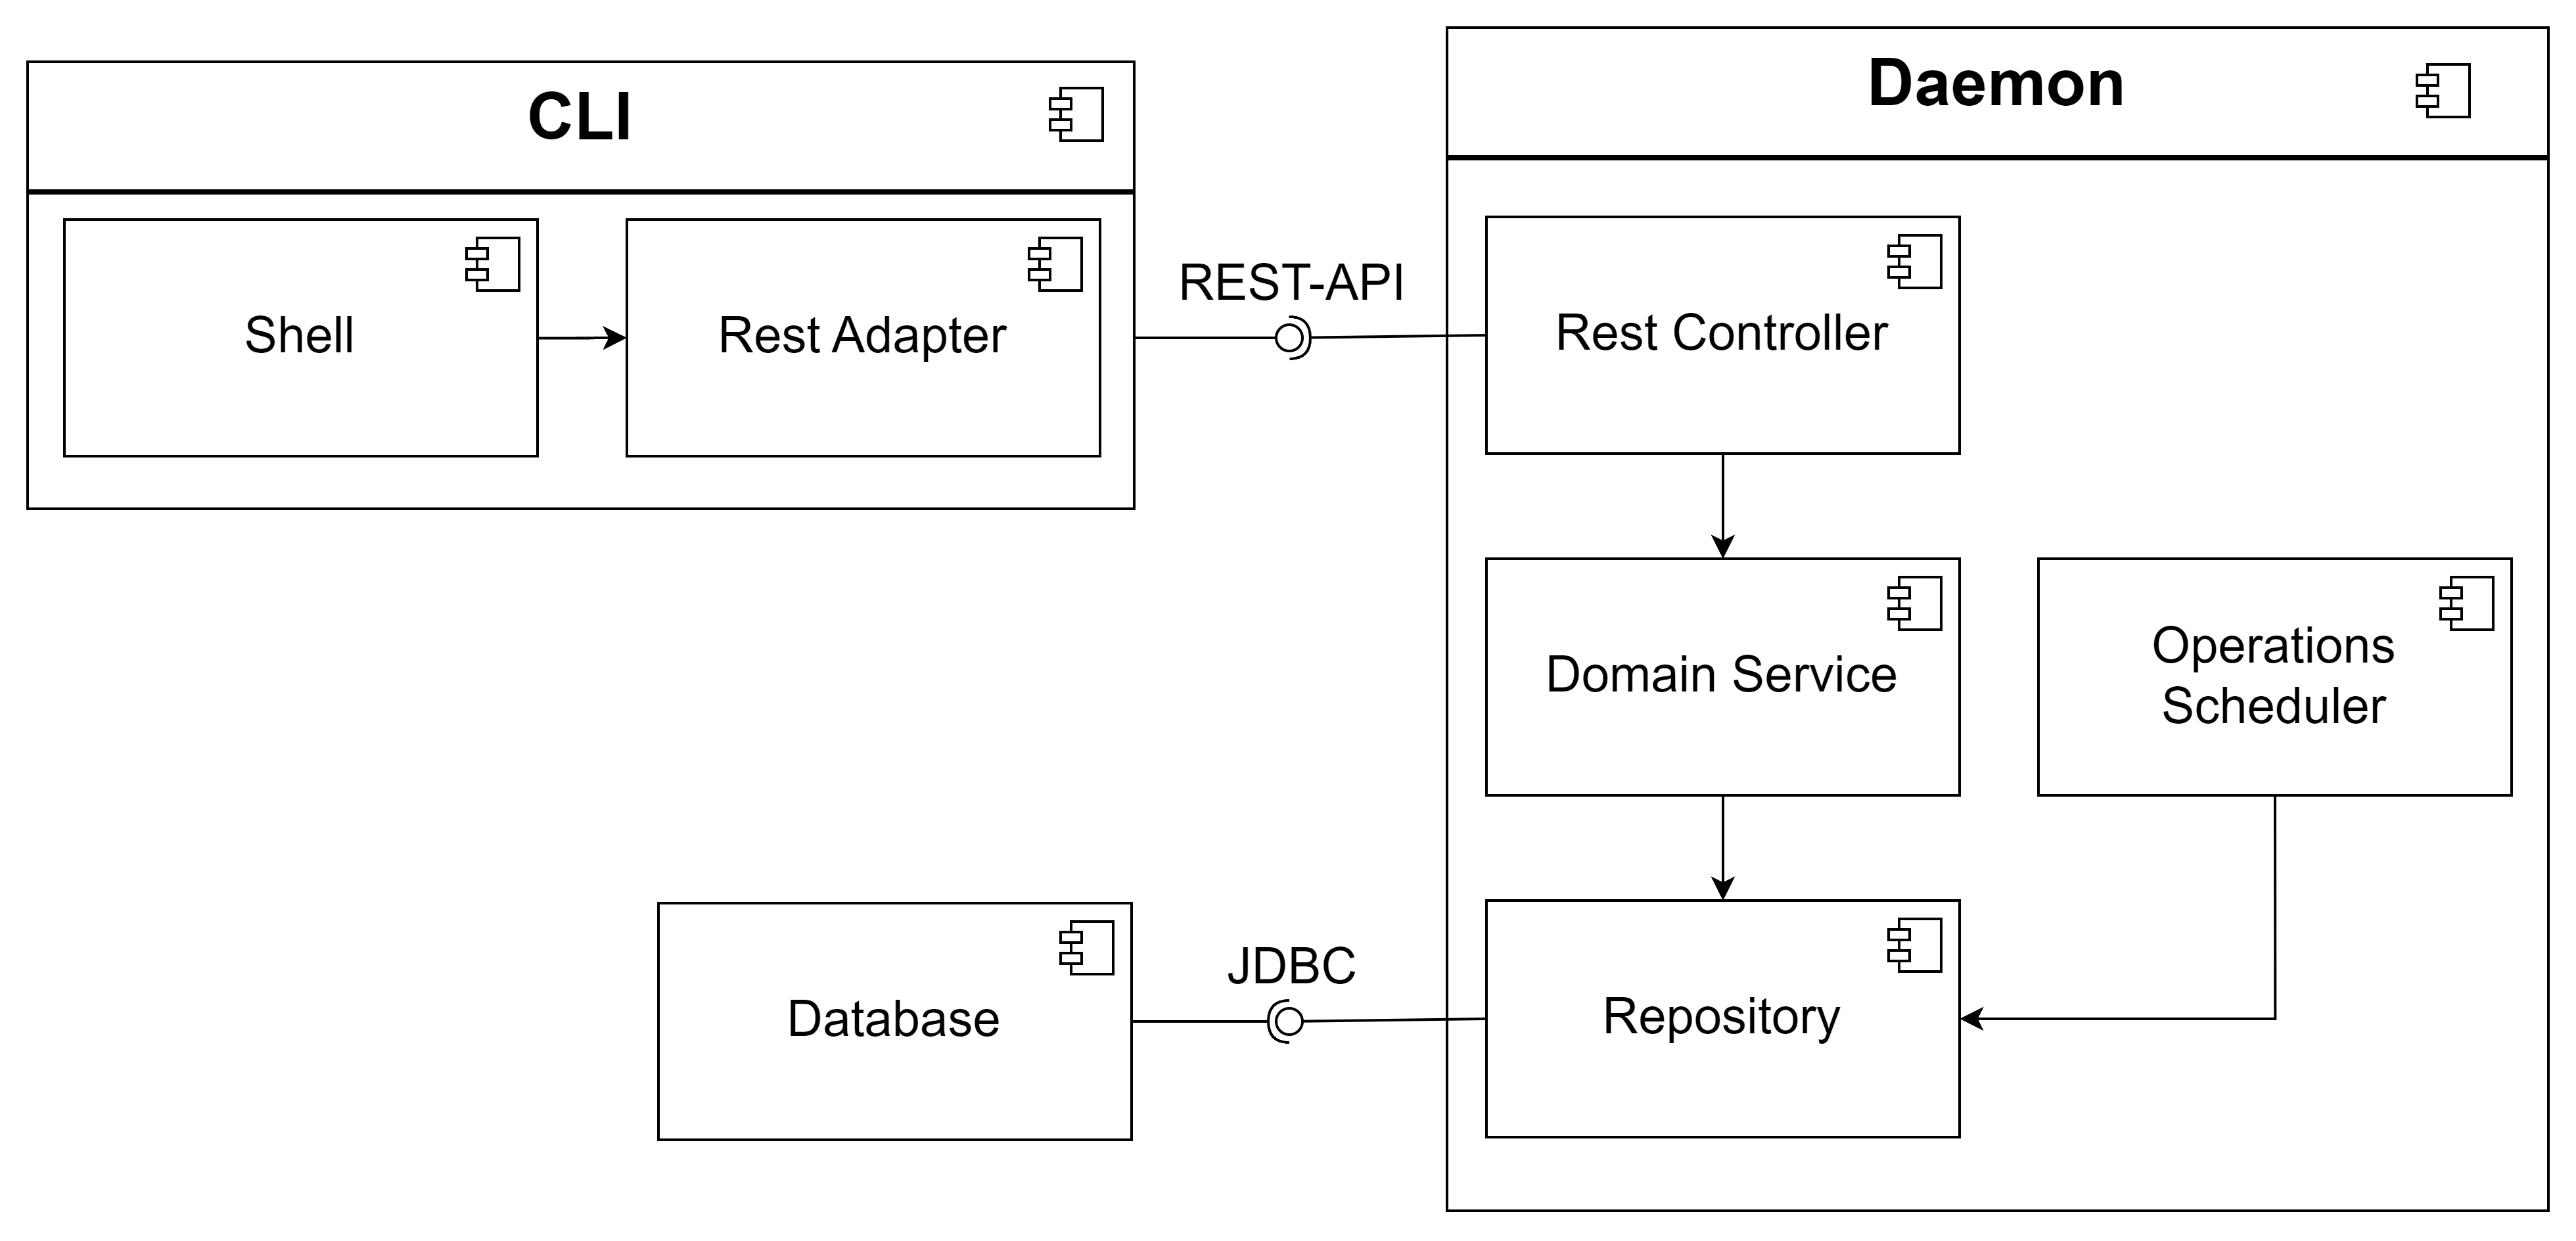
\includegraphics[width=1\textwidth]{assets/comp-diag-tracesentry-v3}
        \caption{UML Komponentendiagramm}
        \label{fig:comp-diag}
        \vspace{2em}
    \end{figure}

    \subsubsection{Domänen}\label{subsubsec:domaenen}
    Die im Diagramm dargestellten Subkomponenten kapseln Funktionalitäten und sind in der Regel in eigenen Klassen implementiert.
    Es können mehrere Instanzen dieser Subkomponenten implementiert werden und nach fachlichen Aspekten, sogenannten Domänen, aufgeteilt werden.
    \\Am Beispiel einer Snapshot-Domäne würden dann im Backend ein Snapshot-(Rest)-Controller, ein Snapshot-(Domain)-Service und ein Snapshot-Repository existieren.
    D.h.\ eine Kapselung findet in technischer und fachlicher Hinsicht statt.
    Eine komplette Abkapselung ist jedoch in der Praxis schwierig und soll lediglich angestrebt werden.\\

    \newpage

    \subsubsection{Shell}\label{subsubsec:shell}
    Die Shell stellt eine Kommandozeilen-Benutzerschnittstelle zur Verfügung.
    Sie kapselt die Definition von Kommandos und deren Parameter.
    Ausserdem übernimmt sie das Parsen der Benutzereingaben, clientseitige Validierung sowie Exception-Handling.

    \subsubsection{Rest Adapter}\label{subsubsec:rest-adapter}
    Der Rest Adapter kapselt Funktionen zur Interaktion mit der REST-Schnittstelle.

    \subsubsection{Rest Controller}
    Der Rest Controller implementiert die Endpunkte der REST-Schnittstelle gemäss \hyperref[sec:api-spec]{API-Spezifikation}.

    \subsubsection{Domain Service}
    Der Domain Service implementiert die Applikations- bzw.\ Geschäftslogik.
    Dazu gehört serverseitige Validierung, Datenverarbeitung und -Persistierung.

    \subsubsection{Operations Scheduler}
    Der Monitoring Scheduler führt periodisch Operationen aus.

    \subsubsection{Repository}
    Das Repository stellt den Zugang zur Persistenzschicht zur Verfügung.
    Dabei handelt es sich um Create, Read, Update, Delete (CRUD) Operationen in Form von Datenbankqueries.

    \subsubsection{Technologien}
    \begin{table}[h!]
        \centering
        \setlength{\leftmargini}{0.4cm}
        \begin{tabular}{|p{5.5cm}|p{5cm}|}
            \hline
            & \textbf{Technologien (primär)} \\
            \hline
            \textbf{Shell}                & Java, Spring (Shell)           \\
            \hline
            \textbf{Rest Adapter}         & Java, Spring (Web)             \\
            \hline
            \textbf{Rest Controller}      & Java, Spring (Web)             \\
            \hline
            \textbf{Domain Service}       & Java, Spring                   \\
            \hline
            \textbf{Operations Scheduler} & Java, Spring                   \\
            \hline
            \textbf{Repository}           & Java, Spring (Data)            \\
            \hline
            \textbf{Database}             & SQLite                         \\
            \hline
        \end{tabular}
        \caption{Technologien der Komponenten}\label{tab:table}
    \end{table}

    \clearpage

    \subsection{Realisierung}\label{subsec:realisierung}
    Die Realisierung ist die Umsetzung der~\nameref{sec:anforderungen} mittels der~\nameref{subsec:loesungsarchitektur}.
    Hauptbaublöcke sind Java-Klassen.
    Geteilte Klassen sind in einer eigenen Bibliothek (\texttt{lib}) ausgelagert.
    Die Klassendiagramme für die CLI, den Daemon und die Lib sind im Anhang unter \hyperref[sec:class-diag-cli]{Klassendiagramm CLI}, \hyperref[sec:class-diag-daemon]{Klassendiagramm Daemon} und \hyperref[sec:class-diag-lib]{Klassendiagramm Lib} zu finden.

    \subsubsection{Frontend (CLI)}\index{CLI}
    \paragraph*{Beispiel Komponenteninteraktion}
    Das folgende Sequenzdiagramm zeigt eine typische Interaktion zwischen Implementationen von Subkomponenten gemäss der~\nameref{subsec:loesungsarchitektur}.
    In diesem Fall handelt es sich um das \texttt{inspect} Kommando (siehe~\nameref{sec:user-manual}).
    Die Klasse InspectCommand ist Teil der Shell (siehe~\nameref{subsubsec:shell}). Der DaemonAdapter ist die Implementation des RestAdapters (siehe~\nameref{subsubsec:rest-adapter}).
    \begin{figure}[h]
        \centering
        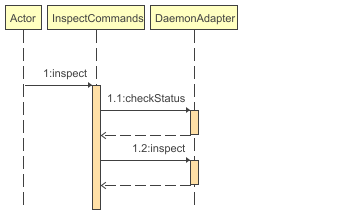
\includegraphics[width=0.7\textwidth]{assets/InspectCommands_inspect_seq_diag}
        \caption{Sequenzdiagramm Inspect Command}
        \label{fig:seq-diag-inspect-commands}
    \end{figure}
    \\Dieses Muster ist für alle Kommandos in der Shell identisch, daher wird dieser Abschnitt in prägnanter Form gehalten.

    \subsubsection{Backend (Daemon)}\index{Daemon}
    \paragraph*{Beispiel Komponenteninteraktion}
    Das folgende Sequenzdiagramm zeigt ebenfalls eine typische Interaktion zwischen Implementationen von Subkomponenten gemäss \\
    der~\nameref{subsec:loesungsarchitektur}.
    Man sieht innerhalb der Monitoring-Domäne den Controller (MonitoringController), den Service (MonitoringDomainService) und das Repository (MonitoredPathRepository).
    Des Weiteren sieht man eine Utility-Klasse (ControllerUtils) und eine Entitätsklasse (MonitoredPath) und zur Veranschaulichung (in rot) die Superklasse vom Spring-Framework (CrudRepository).
    \\In diesem Beispiel wird ein überwachter Pfad (MonitoredPath) erstellt:
    \begin{sidewaysfigure}
        \centering
        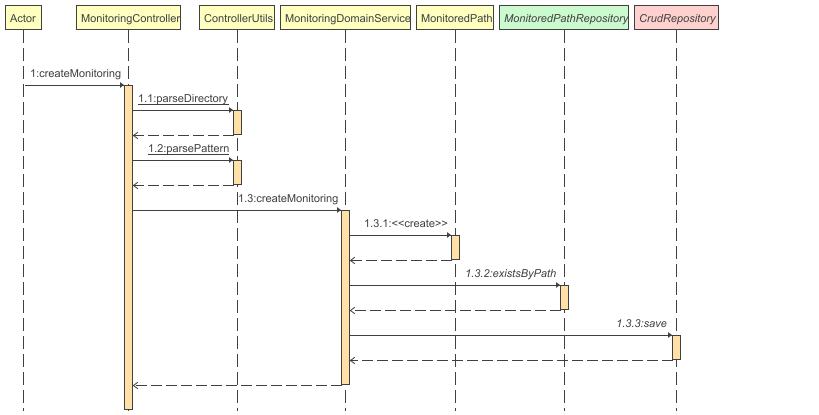
\includegraphics[width=1\textwidth]{assets/MonitoringController_createMonitoring_seq_diag}
        \caption{Sequenzdiagramm Monitoring Controller}
        \label{fig:seq-diag-monitoring-controller}
    \end{sidewaysfigure}

    \clearpage

    \paragraph*{Monitoring}\mbox{}\\
    Der Monitoring Scheduler ist die Implementation des Operations Schedulers (siehe~\nameref{subsec:loesungsarchitektur}).
    Er speichert periodisch Snapshots\index{Snapshots} von überwachten Pfaden in der Datenbank (1.1).
    Für jeden überwachten Pfad wird ein Snapshot (1.1.3), d.h.\ ein Hashbaum, erstellt (1.1.4).\\
    Für jeden Knoten des Baumes werden die Hashes mit dem letzten Snapshot verglichen und ein Flag gesetzt, falls sich der Knoten geändert hat.
    Falls ein Knoten nicht mehr existiert, wird dafür ein Flag im alten Snapshot gesetzt.
    Diese zwei Flags sind die einzigen Felder, die auf Informationen vom Vorgänger (1.1.1, 1.1.2) bzw.\ Nachfolger zurückgreifen,
    alle anderen Felder stellen Informationen des aktuellen Snapshots im Sinne einer Momentaufnahme dar.
    \\Der Intervall für die Periodizität der Snapshot-Erstellung ist konfigurierbar und kann z.B.\ via Programmargument oder Konfigurationsdatei gesetzt
    \\(mit Key \texttt{monitoring-scheduler.snapshot.interval}) werden.
    Standardmässig ist der Wert auf 1 Stunde gesetzt.
    \begin{sidewaysfigure}
        \centering
        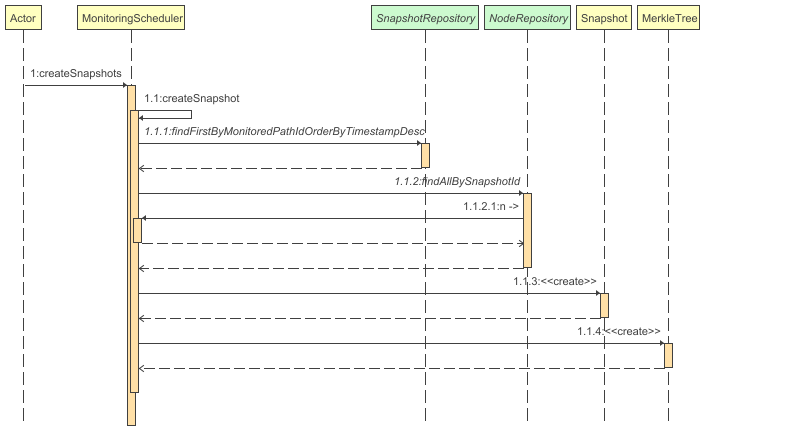
\includegraphics[width=1\textwidth]{assets/MonitoringScheduler_createSnapshots_seq_diag}
        \caption{Sequenzdiagramm Monitoring Scheduler}
        \label{fig:seq-diag-monitoring-scheduler}
    \end{sidewaysfigure}

    \clearpage

    \paragraph*{Optimierungen}\mbox{}\\
    In den folgenden zwei Szenarien wurde geprüft, ob die Implementierung eines \textbf{Caching-Mechanismus} sinnvoll ist.
    Basierend auf den analysierten Aspekten wurde jedoch entschieden, darauf zu verzichten.
    Die Entscheidungsgrundlage wird im Folgenden erläutert:
    \begin{enumerate}
        \item Für jeden \texttt{MonitoredPath} könnte der zuletzt erzeugte Merkle-Tree zwischengespeichert werden, um diesen beim nächsten Snapshot direkt mit dem neuen Baum vergleichen zu können,
        ohne ihn erneut aus der Datenbank laden zu müssen.
        \begin{itemize}
            \item Ein Caching-Ansatz ist nur dann sinnvoll, wenn dieselben Daten mehrfach genutzt werden.
            Da jedoch der Merkle-Tree\index{Merkle-Tree} des letzten Snapshots lediglich einmal (beim Vergleich mit dem neuen Baum) verwendet wird, ergibt sich hieraus kein signifikanter Nutzen.
            \item Der Leistungsgewinn durch Caching wäre im Vergleich zum Laden aus der Datenbank marginal.
            Die Datenbank ist lokal angebunden, und die Abfrage weist eine geringe Komplexität auf, sodass ein effizienter Zugriff bereits gewährleistet ist.
        \end{itemize}
        \item Für jeden \texttt{MonitoredPath} könnte eine geordnete Liste der Änderungen jedes Snapshots im Speicher gehalten werden, um diese direkt zurückgeben zu können,
        ohne auf die Datenbank zugreifen zu müssen.
        \begin{itemize}
            \item Auch in diesem Szenario wird keine nennenswerte Steigerung der Performance erwartet.
            Selbst wenn die Daten bereits im Speicher verfügbar wären, erfordert die Erstellung der zusammengefassten Antwort zusätzliche Logik.
            Diese kann ebenso effizient durch eine Abfrage auf die lokale Datenbank umgesetzt werden, wodurch sich kein signifikanter Vorteil ergibt.
        \end{itemize}
    \end{enumerate}

    \clearpage

    \subsubsection{Merkle-Tree (Hashbaum)}\index{Merkle-Tree
    Ein Merkle-Tree ist eine binäre Baumstruktur, die zur effizienten Überprüfung von Datenintegrität verwendet wird.
    Er eignet sich für das Vergleichen von Baumstrukturen, wie sie in Dateisystemen vorkommen.
    \\Bei der Erstellung eines Snapshots\index{Snapshots} eines überwachten Pfades wird ein eben solcher Baum erstellt.
    Er besteht aus Knoten, die Hashes von Dateien oder Unterverzeichnissen enthalten.
    \\Folgender Pseudocode (stark vereinfacht) zeigt das Erstellen eines Merkle-Trees für einen Snapshot eines überwachten Pfades.

    \begin{lstlisting}[label={lst:merkle-pseudo}]
buildMerkleTree(path, snapshot):
    1. ueberpruefe, ob der Pfad gueltig ist. Falls nicht: Abbrechen.
    2. Erstelle Wurzel-Knoten fuer das Verzeichnis.
    3. Rufe BuildTreeRecursively(Wurzel, snapshot, Verzeichnisinhalte) auf.

buildTreeRecursively(parent, snapshot, files):
    1. Initialisiere eine Liste fuer Kind-Knoten.
    2. Fuer jede Datei im Verzeichnis:
        a. Wenn Datei ein Unterverzeichnis ist:
            - Erstelle Knoten fuer das Verzeichnis.
            - Rufe BuildTreeRecursively fuer das Unterverzeichnis auf.
        b. Wenn Datei gueltig ist (entspricht Filter):
            - Erstelle Knoten fuer die Datei.
        c. Fuege den neuen Knoten zur Kinderliste hinzu.
    3. Kombiniere Hashes aller Kinder und speichere im Elternknoten.

    \end{lstlisting}

    \subsubsection{\textbf{Komplexität}}\index{Merkle-Tree
    Unser System ist von Grund auf auf Effizienz und Performanz ausgelegt, der Hashbaum als zentrale Datenstruktur ermöglicht dies.
    Die Datenmenge mit der ein Benutzer arbeitet, kann sehr gross werden, daher ist es wichtig, dass die Skalierbarkeit des Systems gewährleistet ist.
    Eine Analyse der Komplexität der verschiedenen Operationen des Merkle-Trees ist daher angebracht.
    \\
    Jeder Ordner und jede Datei wird als Knoten im Hashbaum repräsentiert.
    Die Wurzel des Hashbaums repräsentiert den zu überwachenden Pfad.
    Dateien sind stets Blätter.\newline
    Folgend ist $n$ die Anzahl der Knoten im Verzeichnis des zu überwachenden Pfades.

    \paragraph*{Konstruktion}
    Der Baualgorithmus besucht rekursiv alle Dateien und Ordner im zu überwachenden Pfad,
    was einer Komplexität von $O(n)$ für das Traversieren entspricht.
    Das Hashen eines Ordners mit $k$ Kindern setzt eine Iteration über alle Kinder voraus, was einer Komplexität von $O(k)$ entspricht.
    Das Hashen eines Blattes (Datei) ist abhängig von der Grösse $s$ der Datei und hat eine Komplexität von $O(s)$.
    \\\\
    Die Gesamtkomplexität des Bauens des Hashbaums beträgt also $\boldsymbol{O(n \cdot s)}$
    Hier ist $s$ die durchschnittliche Dateigrösse. $k$ ist implizit in $n$ enthalten.

    \paragraph*{Linearisierung}
    Es gibt Fälle, in denen der Hashbaum linearisiert wird, um z.B.\ die Java Stream API zu verwenden oder direkt alle Knoten miteinander zu persistieren.
    Es werden für alle Knoten die Referenzen in einer Liste gespeichert, was einer Komplexität von $\boldsymbol{O(n)}$ entspricht.

    \clearpage

    \subsubsection{Datenbank}\label{subsubsec:realisierung-datenbank}
    Produktiv wird eine SQLite-Datenbank\index{SQLite} verwendet, welche lokal auf dem System des Benutzers in Form einer einzigen *.db-Datei gespeichert wird.
    Für die automatisierten Tests wurde eine H2-In-Memory-Datenbank verwendet, welche für jeden Test mit dem gleichen Schema,
    das auch für die produktive Datenbank verwendet wird jeweils initialisiert wird.

    \paragraph*{Modell}\mbox{}\\
    \begin{figure}[h]
        \centering
        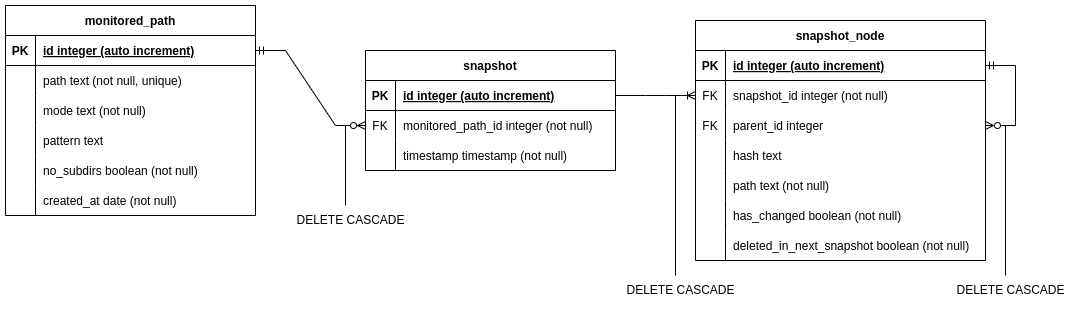
\includegraphics[width=1\textwidth]{assets/erd}
        \caption{Entity Relationship Diagram}
    \end{figure}

    \paragraph*{monitored\_path}\mbox{}\\
    In dieser Tabelle werden die zu überwachenden Pfade mit den dazugehörigen Such-Optionen gespeichert.

    Attribute:
    \begin{itemize}
        \item \textbf{id} (INTEGER): Eindeutige ID des überwachten Pfades.
        \item \textbf{path} (TEXT): Absoluter Pfad des überwachten Verzeichnisses.
        \item \textbf{mode} (TEXT): Gibt an, mit welchem Modus der Pfad durchsucht werden soll.
        \item \textbf{pattern} (TEXT): Regex-Pattern für Dateien, nach denen im Verzeichnis des Pfads gesucht werden soll.
        \item \textbf{no\_subdirs} (BOOLEAN): Gibt an, ob Unterverzeichnisse durchsucht werden sollen.
        \item \textbf{created\_at} (DATE): Zeitpunkt der Erstellung des überwachten Pfades.
    \end{itemize}

    \paragraph*{snapshot}\mbox{}\\
    In dieser Tabelle werden die Snapshots\index{Snapshots} der überwachten Pfade gespeichert,
    welche periodisch mit einem definierten Intervall erstellt werden.

    Attribute:
    \begin{itemize}
        \item \textbf{id} (INTEGER): Eindeutige ID des Snapshots.
        \item \textbf{monitored\_path\_id} (INTEGER): Fremdschlüssel auf den überwachten Pfad.
        Falls der überwachte Pfad gelöscht wird, werden auch alle zugehörigen Snapshots gelöscht.
        \item \textbf{timestamp} (TIMESTAMP): Zeitpunkt der Erstellung des Snapshots.
    \end{itemize}

    \paragraph*{snapshot\_node}\mbox{}\\
    In dieser Tabelle werden die Knoten des Merkle-Trees\index{Merkle-Tree gespeichert, welche die Dateien und Verzeichnisse des überwachten Pfades repräsentieren.
    Durch die Natur von relationalen Datenbanken wird der Baum linearisiert gespeichert und die Beziehungen durch Fremdschlüssel auf die gleiche Entität (Parent-Knoten) rekursiv abgebildet.

    Attribute:
    \begin{itemize}
        \item \textbf{id} (INTEGER): Eindeutige ID des Knotens.
        \item \textbf{snapshot\_id} (INTEGER): Fremdschlüssel auf den Snapshot, zu dem der Knoten gehört.
        Falls der Snapshot gelöscht wird, werden auch alle zugehörigen Knoten gelöscht.
        \item \textbf{parent\_id} (INTEGER): Fremdschlüssel auf den Parent-Knoten.
        Falls der Parent-Knoten gelöscht wird, wird auch der Kind-Knoten gelöscht.
        \item \textbf{hash} (TEXT): Hash der Datei, die von diesem Knoten abgebildet wird.
        \item \textbf{path} (TEXT): Absoluter Pfad der Datei, die von diesem Knotens abgebildet wird.
        \item \textbf{has\_changed} (BOOLEAN): Gibt an, ob sich die Datei, die von diesem Knoten abgebildet wird
        seit dem letzten Snapshot geändert hat oder sie neu hinzugefügt wurde.
        \item \textbf{deleted\_in\_next\_snapshot} (BOOLEAN): Gibt an, ob die Datei, die von diesem Knoten abgebildet wird
        im nächsten Snapshot nicht mehr existiert.
    \end{itemize}

    \paragraph*{Indexing}\mbox{}\\
    Die Entscheidung über die Sinnhaftigkeit eines SQL-Indexes für bestimmte Attribute der Datenbank basierte auf den folgenden Kriterien:

    \textit{Index sinnvoll:}
    \begin{itemize}
        \item Das Attribut weist eine hohe Kardinalität (viele unterschiedliche Werte) auf.
        \item Das Attribut enthält wenige oder keine Null-Werte.
        \item Das Attribut wird häufig in SQL \texttt{WHERE/JOIN}-Klauseln verwendet.
    \end{itemize}

    \textit{Index nicht sinnvoll:}
    \begin{itemize}
        \item Die Tabelle ist von geringer Größe.
        \item Das Attribut wird häufig manipuliert.
    \end{itemize}

    Auf Basis dieser Überlegungen wurden die folgenden Attribute zur Indexierung ausgewählt:
    \begin{itemize}
        \item \texttt{snapshot\_node.snapshot\_id}
        \item \texttt{snapshot\_node.has\_changed}
        \item \texttt{snapshot\_node.deleted\_in\_next\_snapshot}
    \end{itemize}

    \subsubsection{REST-Schnittstelle}\index{REST-API}
    Siehe~\nameref{sec:api-spec} im Anhang.

    \subsubsection{KI-Anbindung}\label{subsubsec:ki-anbindung}
    \paragraph*{Architektur und Funktionsweise}
    Die Anbindung an KI-Modelle erfolgt über den \textit{InspectController}, der die HTTP-Anfragen der CLI entgegennimmt.
    Dieser liest die zu analysierende Datei ein und ruft eine Implementierung des \textit{InspectionService} Interfaces auf, welche für die Kommunikation mit einem spezifischen KI-Modell zuständig ist.

    \begin{figure}[h]
        \centering
        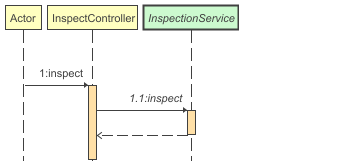
\includegraphics[width=0.7\textwidth]{assets/InspectController_inspect_seq_diag}
        \caption{Sequenzdiagramm InspectController}
        \label{fig:seq-diag-inspect-controller}
    \end{figure}

    Im Rahmen dieses Projekts wurde GPT-4o mini als KI-Modell verwendet
    (Siehe~\nameref{sec:ki-fallstudie}).
    Für dieses Modell wurde der \textit{GPTInspectionService} implementiert, welcher die Anfrage an die OpenAI-API sendet und die Antwort verarbeitet.

    \begin{figure}[h]
        \centering
        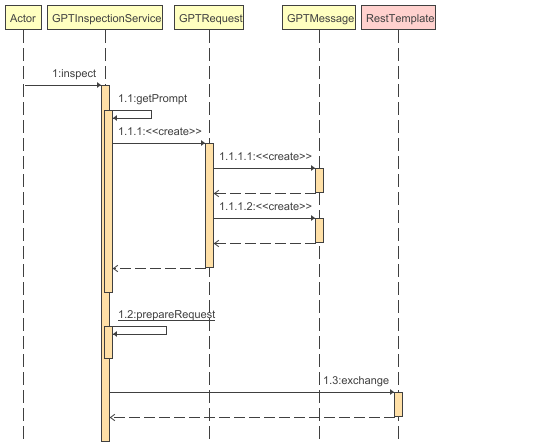
\includegraphics[width=0.7\textwidth]{assets/GPTInspectionService_inspect_seq_diag}
        \caption{Sequenzdiagramm GPTInspectionService}
        \label{fig:seq-diag-gpt-inspection-service}
    \end{figure}

    \clearpage
    \paragraph*{OpenAI Schnittstelle}\label{par:openai-schnittstelle}
    Die Kommunikation mit dem KI-Modell basiert auf REST-API-Calls.
    Um eine Anfrage an die OpenAI-API zu senden, wird ein HTTP-POST-Request an \texttt{https://api.openai.com/v1/chat/completions} gesendet.
    Die Authentifizierung erfolgt über einen API-Key, der im Authorization-Header mitgegeben wird.
    Dieser wird im Vorfeld aus der Umgebungsvariable \texttt{OPENAI\_API\_KEY} ausgelesen.
    Die Anfrage ist wie folgt strukturiert:

    \begin{lstlisting}[language=json,caption={OpenAI Anfrage},label={lst:openai-request}]
    {
      "model": "gpt-4o-mini",
      "messages": [
        {
          "role": "system",
          "content": "<SYSTEM_PROMPT>"
        },
        {
          "role": "user",
          "content": "<userPrompt>"
        }
      ]
    }
    \end{lstlisting}
    Diese Struktur wird durch die Klassen \texttt{GPTRequest} inkl. \texttt{GPTMessage} abgebildet (siehe~\nameref{fig:seq-diag-gpt-inspection-service}).

    Die Antwort der OpenAI Schnittstelle ist deutlich umfangreicher und enthält neben der eigentlichen Antwort auch Metadaten.
    Für die Analyse wird lediglich der Antworttext benötigt, welcher aus der JSON-Response extrahiert wird.

    \begin{lstlisting}[language=json,caption={OpenAI Antwort},label={lst:openai-response}]
    {
      "choices": [
        {
          "message": {
            "content": "<Antwort>"
          }
        },
        {}
      ]
    }
    \end{lstlisting}

    \paragraph*{Prompt-Engineering}
    Die Qualität der Antwort des KI-Modells hängt stark von der Qualität des System- und Benutzer-Prompts ab.
    Beide Prompts werden in derselben Anfrage an die OpenAI-API übergeben.
    Das System-Prompt ist fix und definiert den Kontext, in dem die Antwort generiert wird.
    Das Benutzer-Prompt beinhaltet den absoluten Pfad im Dateisystem sowie den gesamten Inhalt der zu analysierenden Datei.

    \clearpage
    \begin{lstlisting}[label={lst:system-prompt}]
You will receive the entire file content, including its name
and path. These are typically log or cache files. Your task
is to evaluate the file for harmful or problematic features.
Pay close attention to the file's name and path as they may
provide important context.

Respond concisely in **a maximum of 5 sentences**, addressing the following:
1. **Intended use**: Briefly describe the file's purpose based on its content, name, and path. If its content contains suspicious or harmful elements, describe them.
2. **Assessment**: Classify the file as harmful, potentially harmful, or harmless.
3. **Recommended to Wipe**: Suggest one of the following actions: No, Clear file, Delete file.
4. **Additional recommendations**: If necessary, provide additional recommendations or actions.

### Example:
Intended use:
[Describe the file's intended use in up to 10 sentences. Use up
to 10 sentences to describe harmful or suspicious elements.]

Assessment:
[Harmful / Potentially harmful / Harmless]

Recommended to Wipe:
[No / Clear file / Delete file]

Additional recommendations:
[Provide additional recommendations or actions only if
necessary.]
    \end{lstlisting}
    Diese System-Prompt beschreibt bereits die zu erwartende Struktur der Benutzer-Prompt, wie auch die zu erwartende Antwortstruktur.
    Dank dieser ausführlichen System-Prompt erfolgen die Antworten des Modells zuverlässig und konsistent (siehe~\nameref{sec:ki-fallstudie}).

    Benutzer-Prompt: % TODO mit anderen listings abgleichen, DESIGN
    \begin{lstlisting}[label={lst:user-prompt}]
file path: <absoluter Pfad>
file content:
<Inhalt der Datei>
    \end{lstlisting}
    Die Benutzer-Prompt ist bewusst kurz gehalten, damit sich das Modell auf die relevanten Informationen konzentrieren kann.

    \clearpage


    \section{Prozesse}\label{sec:prozesse}
    In diesem Kapitel wird auf die Verwendung der Projektmethode Scrum während des Projekts eingegangen.
    Dabei ist wichtig wie Scrum adaptiert wurde, um so gut wie möglich im vorgegebenen Projektrahmen zu funktionieren.

    \subsection{Rollen}
    \begin{table}[h!]
        \centering
        \setlength{\leftmargini}{0.8cm}
        \begin{tabular}{|c|p{10cm}|}
            \hline
            \textbf{Developer}     & Ganzes Team  \\ \hline
            \textbf{Scrum Master}  & Luca Ammann  \\ \hline
            \textbf{Product Owner} & Luca Scherer \\ \hline
        \end{tabular}
        \caption{Scrum Rollen}\label{tab:scrum-roles}
    \end{table}
    Wir versuchen alle zu entwickeln und dabei die Arbeitslast mit Rücksicht auf die
    zusätzlichen Aufgaben der SM- und PO-Rollen so gleichmässig wie möglich zu verteilen.

    \subsubsection*{Weitere Rollen}
    \begin{table}[h!]
        \centering
        \setlength{\leftmargini}{0.8cm}
        \begin{tabular}{|c|p{10cm}|}
            \hline
            \textbf{Berater}    & Dr. Simon Kramer \\ \hline
            \textbf{PM-Berater} & Frank Helbling   \\ \hline
        \end{tabular}
        \caption{Weitere Rollen}\label{tab:additional-roles}
    \end{table}

    \subsection{Sprintziele}
    Die Sprintziele wurden jeweils nach dem SMART-Prinzip definiert.
    Dazu folgende zwei Beispiele:
    \begin{itemize}
        \item Aufsetzen von lauffähiger CLI- und Daemon-Komponente und vollständige, sowie getestete Implementation der Search-Funktion (gemäss Testkonzept).
        \item Monitoring-Kommandos (gemäss Spezifikation) für das Persistieren und Auflisten der Dateipfade sind vollständig implementiert und getestet (gemäss Testkonzept).
    \end{itemize}

    \subsection{Anwendung}

    \subsubsection{Sprints}
    Die Sprints leben auf Stufe einer Group in Gitlab.
    Sie werden als Iterations bezeichnet.
    Issues können explizit zu einer Iteration zugewiesen werden.

    \clearpage

    \subsubsection{Epics}
    Epics werden in Gitlab auf Stufe einer Group verwaltet.
    User Stories können zu einem Epic promoted werden.
    Epics sind grob beschrieben und kapseln mehrere kohärente Funktionen in Form von User Stories.
    Dazu folgendes Beispiel:
    \begin{figure}[h]
        \centering
        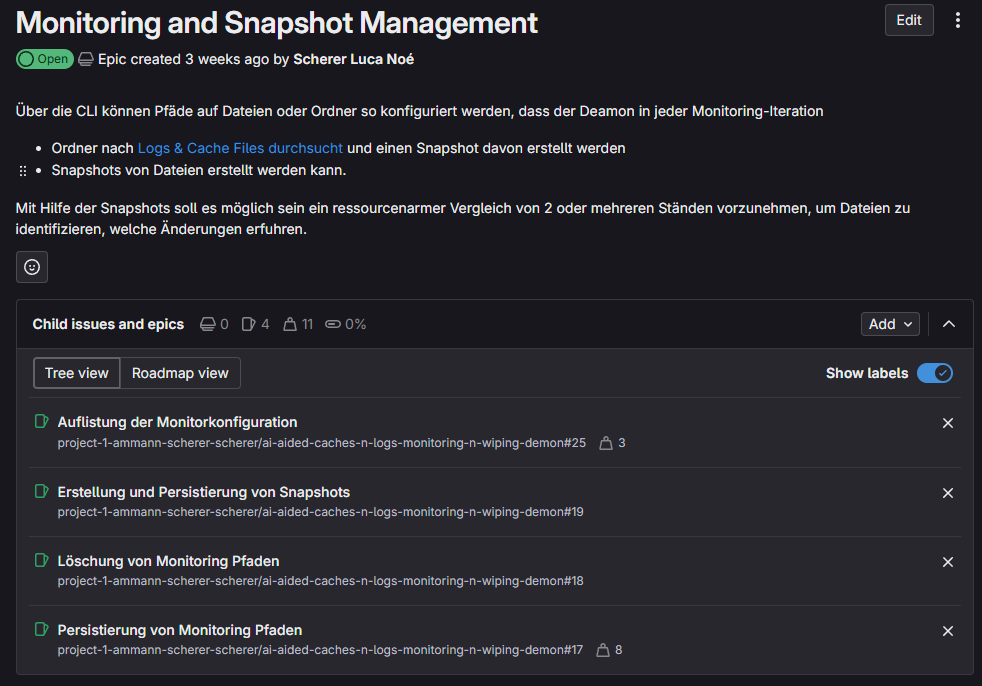
\includegraphics[width=1\textwidth]{assets/epic-example}
        \caption{Epic Beispiel}
        \label{fig:epic-example}
    \end{figure}

    \clearpage

    \subsubsection{User Stories}
    Eine User Story wird in Gitlab als Issue bezeichnet.
    Sie lebt auf der Stufe eines Projektes (Repository) und kann einem Epic zugeordnet sein.
    Sie kann ebenfalls sogenannte Tasks enthalten, welche kleinere Arbeiten der User Stories (meistens aus Entwickler-Sicht) repräsentieren.
    Jede User Story ist gemäß folgendem Schema dokumentiert:
    \\
    \texttt{Als <Benutzerrolle> möchte ich <Funktion>, sodass <Begründung/Benefit>.}
    Dazu folgendes Beispiel:
    \begin{figure}[h]
        \centering
        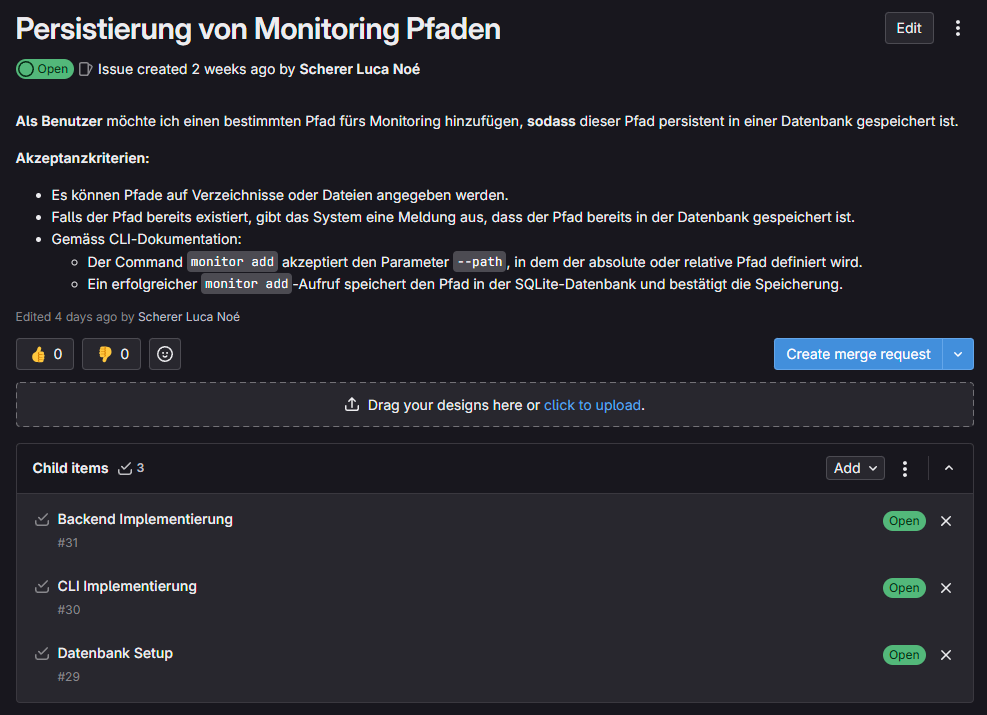
\includegraphics[width=1\textwidth]{assets/user-story-example}
        \caption{User-Story Beispiel}
        \label{fig:user-story-example}
    \end{figure}

    \subsubsection{Definition of Ready}
    Damit eine User Story in ein Sprint Backlog gezogen werden darf, muss sie die Definition of Ready erfüllen.
    Wir haben diese, anlehnend an die INVEST-Kriterien, wie folgt definiert:
    \begin{itemize}
        \item \textbf{Independent:} if possible, a user story should not depend on other user stories.
        \item \textbf{Estimable:} The story must be possible to estimate, and an estimate in Story Points is provided.
        \item \textbf{Small:} The effort for the implementation should be manageable.
        A few hours to a max of a few days.
        \item \textbf{Testable:} Their successful implementation should be verifiable with objective criteria.
        Every story must have acceptance criteria.
        \item Does not violate a non-functional requirement (provided in the project report).
    \end{itemize}

    \subsubsection{Definition of Done}
    Damit eine User Story in die Closed-Spalte gezogen werden darf, muss nachfolgende Definition of Done erreicht sein:
    \begin{itemize}
        \item Pull (Merge) Request is approved by another developer.
        Code Review is done.
        \item Acceptance criteria met.
        \item Functionality tested by someone who was not involved in the story as a developer.
        \item Documentation is done.
    \end{itemize}

    \subsubsection{Taskboard}
    Das Taskboard lebt ebenfalls in unserem Gitlab Project.
    Es beinhaltet folgende Spalten: Open (Product Backlog), Sprint Backlog, Spalte pro Entwickler sowie die Spalte Closed.
    Dies ist die empfohlene Vorgehensweise, da Gitlab so automatisch versteht, welche Issues in welchen Sprint gezogen und auch darin erledigt wurden.
    Gitlab kann so beispielsweise, ohne jegliche Konfigurationen, Burndowncharts pro Iteration erstellen.
    Dazu folgendes Beispiel:
    \begin{figure}[h]
        \centering
        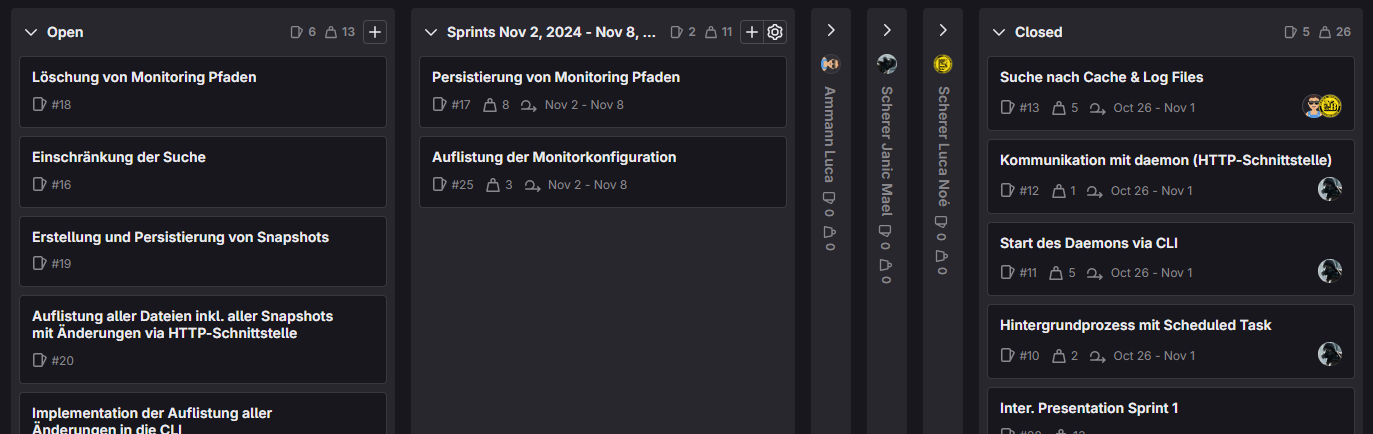
\includegraphics[width=1\textwidth]{assets/issue-board-example}
        \caption{Taskboard Beispiel}
        \label{fig:issue-board-example}
    \end{figure}

    \subsection{Adaptionen}
    Die \textbf{Sprint-Dauer} haben wir auf \textbf{1 Woche} gesetzt, um so in Bezug auf Änderungen
    schneller reagieren zu können, da unsere Projektdauer eher kurz ist im Vergleich zu
    vielen anderen Scrum-Projekten.
    Ausserdem können wir so jede Woche den aktuellen Stand und vor allem die Neuerungen besprechen.
    Das hilft uns, unseren Fokus auf das Ziel und die Deadlines zu halten.
    \\\\
    Das \textbf{Daily} können wir aufgrund unserer beschränkten Zeit, die wir am Projekt arbeiten können, nicht täglich durchführen.
    Dafür sind wir fast täglich per Chat im Austausch und können so kurzfristig, je nach Gebrauch, Besprechungen per Video-Call planen.
    \\\\
    Die \textbf{Scrum-Zeremonien} (Review, Retro, Planning) führen wir en bloc \textbf{jeden Freitag} zum
    Sprint-Abschluss durch und starten sogleich den nächsten geplanten Sprint.


    \chapter{Evaluation und Tests}


    \section{Manuelle End-2-End Tests}\label{sec:manuelle-end-2-end-tests}
    Wie durch das Testkonzept definiert, wurden die End-2-End Tests auf mehreren Endgeräten manuell durchgeführt.

    \subsection{Testfälle}

    \begin{table}[h!]
        \centering
        \setlength{\leftmargini}{0.8cm}
        \begin{tabular}{|c|p{10cm}|}
            \hline
            \textbf{ID}                  & E2E-001                                    \\ \hline
            \textbf{Beschreibung}        & Daemon starten und stoppen                 \\ \hline
            \textbf{Vorbedingungen} &
            \begin{itemize}
                \item Daemon läuft nicht
            \end{itemize} \\ \hline
            \textbf{Ablauf} &
            \begin{enumerate}
                \item \begin{verbatim}ts status
                \end{verbatim}
                \item Erwartet: \begin{verbatim}daemon is not running
                \end{verbatim}
                \item \begin{verbatim}ts run
                \end{verbatim}
                \item \begin{verbatim}ts status
                \end{verbatim}
                \item Erwartet: \begin{verbatim}daemon is running
                \end{verbatim}
                \item \begin{verbatim}ts kill
                \end{verbatim}
                \item \begin{verbatim}ts status
                \end{verbatim}
                \item Erwartet: \begin{verbatim}daemon is not running
                \end{verbatim}
            \end{enumerate} \\ \hline
            \textbf{Erwartetes Ergebnis} & Daemon kann gestartet und gestoppt werden. \\ \hline
        \end{tabular}
        \caption{Manueller End-2-End Test E2E-001}\label{tab:e2e-1}
    \end{table}

    \clearpage

    \begin{table}[h!]
        \centering
        \setlength{\leftmargini}{0.8cm}
        \begin{tabular}{|c|p{10cm}|}
            \hline
            \textbf{ID}                  & E2E-002                              \\ \hline
            \textbf{Beschreibung}        & Autostart                            \\ \hline
            \textbf{Vorbedingungen} &
            \begin{itemize}
                \item Autostart Konfiguration gem.\ Installationshandbuch
            \end{itemize} \\ \hline
            \textbf{Ablauf} &
            \begin{enumerate}
                \item System neustarten
                \item \begin{verbatim}ts status
                \end{verbatim}
                \item Erwartet: \begin{verbatim}daemon is running
                \end{verbatim}
            \end{enumerate} \\ \hline
            \textbf{Erwartetes Ergebnis} & Daemon wird via Autostart gestartet. \\ \hline
        \end{tabular}
        \caption{Manueller End-2-End Test E2E-002}\label{tab:e2e-2}
    \end{table}

    \begin{table}[h!]
        \centering
        \setlength{\leftmargini}{0.8cm}
        \begin{tabular}{|c|p{10cm}|}
            \hline
            \textbf{ID}                  & E2E-003                                                \\ \hline
            \textbf{Beschreibung}        & Inspect                                                \\ \hline
            \textbf{Vorbedingungen} &
            \begin{itemize}
                \item OPENAI\_API\_KEY Umgebungsvariable gesetzt gem.\ Installationshandbuch
                \item Daemon läuft
                \item Beispiel-Datei unter [PFAD] vorhanden
            \end{itemize} \\ \hline
            \textbf{Ablauf} &
            \begin{enumerate}
                \item \begin{verbatim}ts inspect [PFAD]
                \end{verbatim}
                \item Erwartet:
                \begin{verbatim}
Intended use:
The file ...

Assessment:
...

Recommended to Wipe:
...

Additional recommendations:
...
                \end{verbatim}
            \end{enumerate} \\ \hline
            \textbf{Erwartetes Ergebnis} & Einschätzung und Empfehlung von der KI wird angezeigt. \\ \hline
        \end{tabular}
        \caption{Manueller End-2-End Test E2E-003}\label{tab:e2e-3}
    \end{table}

    \clearpage

    \begin{table}[h!]
        \centering
        \setlength{\leftmargini}{0.8cm}
        \begin{tabular}{|c|p{10cm}|}
            \hline
            \textbf{ID}                  & E2E-004                                                                         \\ \hline
            \textbf{Beschreibung}        & Pfad zum Überwachen hinzufügen und entfernen                                    \\ \hline
            \textbf{Vorbedingungen} &
            \begin{itemize}
                \item Daemon läuft
                \item  Der [PFAD] wurde noch nicht hinzugefügt
            \end{itemize} \\ \hline
            \textbf{Ablauf} &
            \begin{enumerate}
                \item \begin{verbatim}ts monitor add [PFAD]
                \end{verbatim}
                \item Erwartet: \begin{verbatim}Successfully added [PFAD]
to the monitoring database.
                \end{verbatim}
                \item \begin{verbatim}ts monitor list
                \end{verbatim}
                \item Erwartet: Der hinzugefügte Pfad wird aufgelistet.
                [ID] des Pfades notieren.
                \item \begin{verbatim}ts monitor remove [ID]
                \end{verbatim}
                \item Erwartet: \begin{verbatim}Successfully removed path with ID [ID]
from the monitoring database.
                \end{verbatim}
                \item \begin{verbatim}ts monitor list
                \end{verbatim}
                \item Erwartet: Der gelöschte Pfad wird nicht mehr aufgelistet.
            \end{enumerate} \\ \hline
            \textbf{Erwartetes Ergebnis} & Ein Pfad kann ohne Fehler hinzugefügt und anschliessend wieder entfernt werden. \\ \hline
        \end{tabular}
        \caption{Manueller End-2-End Test E2E-004}\label{tab:e2e-4}
    \end{table}

    \clearpage

    \begin{table}[h!]
        \centering
        \setlength{\leftmargini}{0.8cm}
        \begin{tabular}{|c|p{10cm}|}
            \hline
            \textbf{ID}                  & E2E-005                                                        \\ \hline
            \textbf{Beschreibung}        & Pfad zum Überwachen mit Mode und ohne Unterordner hinzufügen.  \\ \hline
            \textbf{Vorbedingungen} &
            \begin{itemize}
                \item Daemon läuft
                \item  Der [PFAD] wurde noch nicht hinzugefügt
            \end{itemize} \\ \hline
            \textbf{Ablauf} &
            \begin{enumerate}
                \item \begin{verbatim}ts monitor add [PFAD]
--mode log --no-subdirs
                \end{verbatim}
                \item Erwartet: \begin{verbatim}Successfully added [PFAD] to the
monitoring database.
                \end{verbatim}
                \item \begin{verbatim}ts monitor list
                \end{verbatim}
                \item Erwartet: Pfad wird mit mode=LOG und no-subdirs=true aufgelistet.
            \end{enumerate} \\ \hline
            \textbf{Erwartetes Ergebnis} & Ein Pfad kann mit den gewünschten Optionen hinzugefügt werden. \\ \hline
        \end{tabular}
        \caption{Manueller End-2-End Test E2E-005}\label{tab:e2e-5}
    \end{table}

    \begin{table}[h!]
        \centering
        \setlength{\leftmargini}{0.8cm}
        \begin{tabular}{|c|p{10cm}|}
            \hline
            \textbf{ID}                  & E2E-006                                                               \\ \hline
            \textbf{Beschreibung}        & Pfad zum Überwachen mit Regex-Pattern hinzufügen.                     \\ \hline
            \textbf{Vorbedingungen} &
            \begin{itemize}
                \item Daemon läuft
                \item  Der [PFAD] wurde noch nicht hinzugefügt
            \end{itemize} \\ \hline
            \textbf{Ablauf} &
            \begin{enumerate}
                \item \begin{verbatim}ts monitor add [PFAD] --mode pattern
--pattern ^ts_.*_ts$
                \end{verbatim}
                \item Erwartet: \begin{verbatim}Successfully added [PFAD] to the
monitoring database.
                \end{verbatim}
                \item \begin{verbatim}ts monitor list
                \end{verbatim}
                \item Erwartet: Pfad wird mit pattern=\begin{verbatim}^ts_.*_ts$
                \end{verbatim} aufgelistet.
            \end{enumerate} \\ \hline
            \textbf{Erwartetes Ergebnis} & Ein Pfad kann mit einem gewünschten Regex-Pattern hinzugefügt werden. \\ \hline
        \end{tabular}
        \caption{Manueller End-2-End Test E2E-006}\label{tab:e2e-6}
    \end{table}

    \clearpage

    \begin{table}[h!]
        \centering
        \setlength{\leftmargini}{0.8cm}
        \begin{tabular}{|c|p{10cm}|}
            \hline
            \textbf{ID} & E2E-007 \\ \hline
            \textbf{Beschreibung} & Snapshots generieren lassen und vergleichen. \\ \hline
            \textbf{Vorbedingungen} &
            \begin{itemize}
                \item Daemon läuft
                \item Der [PFAD] wurde noch nicht hinzugefügt.
                (Empfohlen: ein nicht zu tiefer Pfad, damit die Snapshots schneller generiert werden)
            \end{itemize} \\ \hline
            \textbf{Ablauf} &
            \begin{enumerate}
                \item \begin{verbatim}ts monitor add [PFAD] && ts monitor list
                \end{verbatim}
                \item Erwartet: Auflistung des zu überwachenden Pfads, sowie dessen [ID].
                \item \begin{verbatim}ts kill && ts run
                \end{verbatim}
                \item Warten bis Snapshot in Datenbank vorhanden ist.
                Mit nachfolgendem Schritt überprüfen.
                \item \begin{verbatim}ts snapshots list [ID]
                \end{verbatim}
                \item Erwartet: Liste mit genau 1 Snapshot.
                \item Eine Datei test.log in [PFAD] erstellen und mit Inhalt füllen.
                \item \begin{verbatim}ts kill && ts run
                \end{verbatim}
                \item Warten bis zweiter Snapshot in Datenbank vorhanden ist.
                Mit nachfolgendem Schritt überprüfen.
                \item \begin{verbatim}ts snapshots list [ID]
                \end{verbatim}
                \item Erwartet: Liste mit genau 2 Snapshots.
                \item \begin{verbatim}ts snapshots compare [ID]
                \end{verbatim}
                \item Erwartet: Unterschied in der Datei test.log wird aufgelistet.
                \item \begin{verbatim}ts kill && ts run
                \end{verbatim}
                \item Warten bis in Datenbank genau 3 Snapshots vorhanden sind.
                (siehe oben)
                \item \begin{verbatim}ts kill && ts run
                \end{verbatim}
                \item Warten bis in Datenbank genau 4 Snapshots vorhanden sind.
                (siehe oben)
                \item Den Inhalt der Datei test.log ändern.
                \item \begin{verbatim}ts kill && ts run
                \end{verbatim}
                \item Warten bis in Datenbank genau 5 Snapshots vorhanden sind.
                (siehe oben)
            \end{enumerate} \\ \hline
        \end{tabular}\label{tab:e2e-7.1}
    \end{table}
    \clearpage

    \begin{table}[h!]
        \centering
        \setlength{\leftmargini}{0.8cm}
        \begin{tabular}{|c|p{10cm}|}
            \hline
            \textbf{Ablauf} &
            \begin{enumerate}
                \setcounter{enumi}{20}
                \item \begin{verbatim}ts snapshots compare [ID]
                \end{verbatim}
                \item Erwartet: Unterschied in der Datei test.log wird aufgelistet.
                HIER
                \item test.log löschen.
                \item \begin{verbatim}ts kill && ts run
                \end{verbatim}
                \item Warten bis in Datenbank genau 6 Snapshots vorhanden sind.
                \item \begin{verbatim}ts snapshots compare [ID]
                \end{verbatim}
                \item Erwartet: Löschung der Datei test.log wird aufgelistet.
            \end{enumerate} \\ \hline
            \textbf{Erwartetes Ergebnis} & Snapshots werden generiert und drei verschiedenen Zeitintervalle verglichen.
            Erstellung, Änderung und Löschung einer Datei werden erkannt. \\ \hline
        \end{tabular}
        \caption{Manueller End-2-End Test E2E-007}\label{tab:e2e-7.2}
    \end{table}

    \clearpage

    \begin{table}[h!]
        \centering
        \setlength{\leftmargini}{0.8cm}
        \begin{tabular}{|c|p{10cm}|}
            \hline
            \textbf{ID}                  & E2E-008                                            \\ \hline
            \textbf{Beschreibung}        & Search (Cache- und Log-Dateien)                    \\ \hline
            \textbf{Vorbedingungen} &
            \begin{itemize}
                \item Daemon läuft
                \item Beispiel-Verzeichnis unter [PFAD] vorhanden
            \end{itemize} \\ \hline
            \textbf{Ablauf} &
            \begin{enumerate}
                \item \begin{verbatim}ts search [PFAD]
                \end{verbatim}
                \item Erwartet: Auflistung der Inhalte unter [PFAD] welche \("\)cache\("\) oder \("\)log\("\) enthalten.
            \end{enumerate} \\ \hline
            \textbf{Erwartetes Ergebnis} & Auflistung von Dateiinhalten in einem Verzeichnis. \\ \hline
        \end{tabular}
        \caption{Manueller End-2-End Test E2E-008}\label{tab:e2e-8}
    \end{table}

    \begin{table}[h!]
        \centering
        \setlength{\leftmargini}{0.8cm}
        \begin{tabular}{|c|p{10cm}|}
            \hline
            \textbf{ID}                  & E2E-009                          \\ \hline
            \textbf{Beschreibung}        & Leeren und Löschen einer Datei   \\ \hline
            \textbf{Vorbedingungen} &
            \begin{itemize}
                \item Datei unter [PFAD] ist nicht geschützt. (z.B.\ durch Berechtigungen)
                \item Daemon läuft
            \end{itemize} \\ \hline
            \textbf{Ablauf} &
            \begin{enumerate}
                \item \begin{verbatim}ts wipe [PFAD]
                \end{verbatim}
                \item Erwartet: \begin{verbatim}Successfully cleared file.
                \end{verbatim}
                \item Erwartet: Datei wurde geleert
                \item \begin{verbatim}ts wipe [PFAD] --remove
                \end{verbatim}
                \item Erwartet: \begin{verbatim}Successfully removed file.
                \end{verbatim}
                \item Erwartet: Datei wurde gelöscht
            \end{enumerate} \\ \hline
            \textbf{Erwartetes Ergebnis} & Datei wird geleert und gelöscht. \\ \hline
        \end{tabular}
        \caption{Manueller End-2-End Test E2E-009}\label{tab:e2e-9}
    \end{table}

    \clearpage

    \subsection{Testergebnisse}
    \begin{table}[h!]
        \centering
        \setlength{\leftmargini}{0.4cm}
        \begin{tabular}{|c|c|c|c|}
            \hline
            \textbf{Datum} & \textbf{Betriebssystem} & \textbf{Testfall} & \textbf{Ergebnis} \\ \hline
            26.12.2024     & Windows 11--10.0        & E2E-001           & Erfolgreich       \\ \hline
            26.12.2024     & Linux 6.1.0-28          & E2E-001           & Erfolgreich       \\ \hline
            26.12.2024     & macOS Sequoia 15.2      & E2E-001           & Erfolgreich       \\ \hline
            26.12.2024     & Windows 11--10.0        & E2E-002           & Erfolgreich       \\ \hline
            26.12.2024     & Linux 6.1.0-28          & E2E-002           & Erfolgreich       \\ \hline
            26.12.2024     & macOS Sequoia 15.2      & E2E-002           & Erfolgreich       \\ \hline
            26.12.2024     & Windows 11--10.0        & E2E-003           & Erfolgreich       \\ \hline
            26.12.2024     & Linux 6.1.0-28          & E2E-003           & Erfolgreich       \\ \hline
            26.12.2024     & macOS Sequoia 15.2      & E2E-003           & Erfolgreich       \\ \hline
            26.12.2024     & Windows 11--10.0        & E2E-004           & Erfolgreich       \\ \hline
            26.12.2024     & Linux 6.1.0-28          & E2E-004           & Erfolgreich       \\ \hline
            26.12.2024     & macOS Sequoia 15.2      & E2E-004           & Erfolgreich       \\ \hline
            26.12.2024     & Windows 11--10.0        & E2E-005           & Erfolgreich       \\ \hline
            26.12.2024     & Linux 6.1.0-28          & E2E-005           & Erfolgreich       \\ \hline
            26.12.2024     & macOS Sequoia 15.2      & E2E-005           & Erfolgreich       \\ \hline
            26.12.2024     & Windows 11--10.0        & E2E-006           & Erfolgreich       \\ \hline
            26.12.2024     & Linux 6.1.0-28          & E2E-006           & Erfolgreich       \\ \hline
            26.12.2024     & macOS Sequoia 15.2      & E2E-006           & Erfolgreich       \\ \hline
            26.12.2024     & Windows 11--10.0        & E2E-007           & Erfolgreich       \\ \hline
            26.12.2024     & Linux 6.1.0-28          & E2E-007           & Erfolgreich       \\ \hline
            26.12.2024     & macOS Sequoia 15.2      & E2E-007           & Erfolgreich       \\ \hline
            26.12.2024     & Windows 11--10.0        & E2E-008           & Erfolgreich       \\ \hline
            26.12.2024     & Linux 6.1.0-28          & E2E-008           & Erfolgreich       \\ \hline
            26.12.2024     & macOS Sequoia 15.2      & E2E-008           & Erfolgreich       \\ \hline
            26.12.2024     & Windows 11--10.0        & E2E-009           & Erfolgreich       \\ \hline
            26.12.2024     & Linux 6.1.0-28          & E2E-009           & Erfolgreich       \\ \hline
            26.12.2024     & macOS Sequoia 15.2      & E2E-009           & Erfolgreich       \\ \hline

        \end{tabular}
        \caption{Manuelle End-2-End Testergebnisse}\label{tab:e2e-results}
    \end{table}


    \clearpage


    \section{Messungen (Performanztests)}\label{sec:performanztests}
    Um eine Aussage über die Performanz unseres Systems zu machen, haben wir einige Performanztests durchgeführt.
    Diese dienen lediglich als Indikator und sind nicht repräsentativ für alle möglichen Szenarien.
    Es werden nur Kernfunktionen getestet, die Performanz kritisch sein könnten.

    \subsection{Suchfunktion}\label{subsec:testduchfuhrung}
    Es wird im Modus FULL (Cache- und Logdateien) im spezifizierten Pfad nach Dateien gesucht.

    \subsubsection{Verwendete Umgebungsangaben und Metriken}\label{subsubsec:search-perftest-metrics-title}
    \begin{table}[h!]
        \centering
        \setlength{\leftmargini}{0.8cm}
        \begin{tabular}{|p{7cm}|p{7cm}|}
            \hline
            \textbf{System}                                            & Betriebssystem und Architektur                                                  \\ \hline
            \textbf{Pfad}                                              & Verzeichnis, in dem gesucht wird                                                \\ \hline
            \textbf{Anz. Dateien im Pfad}                              & Anzahl Dateien im Pfad (mit allen Unterverzeichnissen)                          \\ \hline
            \textbf{Anz. Verzeichnisse im Pfad}                        & Anzahl Unterverzeichnisse                                                       \\ \hline
            \textbf{Anz. Ebenen \newline des Baumes relevanter Knoten} & Anzahl Ebenen im konstruierten Baum aller gefundenen Dateien und Verzeichnissen \\ \hline
            \textbf{Anz. Knoten \newline des Baumes relevanter Knoten} & Anzahl Knoten im konstruierten Baum aller gefundenen Dateien und Verzeichnissen \\ \hline
            \textbf{Gefundene Dateien}                                 & Anzahl Dateien, die gefunden wurden                                             \\ \hline
            \textbf{Dauer (Stichprobenmittel)}                         & Mittelwert der Dauer in Millisekunden aus mehreren Stichproben                  \\ \hline
        \end{tabular}
        \caption{Beschreibung Umgebungsangaben und Metriken Suchfunktion-Performanztest}\label{tab:perf-search-metrics}
    \end{table}

    \newpage

    \subsubsection{Ergebnisse}
    \begin{table}[h!]
        \centering
        \setlength{\leftmargini}{0.8cm}
        \begin{tabular}{|p{7cm}|p{5cm}|}
            \hline
            \textbf{System}                                            & Windows 11--10.0 / amd64 \\ \hline
            \textbf{Pfad}                                              & C:\textbackslash Windows \\ \hline
            \textbf{Anz. Dateien im Pfad}                              & 188'428                  \\ \hline
            \textbf{Anz. Verzeichnisse im Pfad}                        & 51'184                   \\ \hline
            \textbf{Anz. Ebenen \newline des Baumes relevanter Knoten} & 14                       \\ \hline
            \textbf{Anz. Knoten \newline des Baumes relevanter Knoten} & 54'682                   \\ \hline
            \textbf{Gefundene Dateien}                                 & 3'455                    \\ \hline
            \textbf{Dauer (Stichprobenmittel)}                         & 8'800ms                  \\ \hline
        \end{tabular}
        \caption{Performanztest Suche WIN-1}\label{tab:perf-search-win-1}
    \end{table}

    \begin{table}[h!]
        \centering
        \setlength{\leftmargini}{0.8cm}
        \begin{tabular}{|p{7cm}|p{5cm}|}
            \hline
            \textbf{System}                                            & Windows 11--10.0 / amd64       \\ \hline
            \textbf{Pfad}                                              & C:\textbackslash Program Files \\ \hline
            \textbf{Anz. Dateien im Pfad}                              & 66'386                         \\ \hline
            \textbf{Anz. Verzeichnisse im Pfad}                        & 8'925                          \\ \hline
            \textbf{Anz. Ebenen \newline des Baumes relevanter Knoten} & 20                             \\ \hline
            \textbf{Anz. Knoten \newline des Baumes relevanter Knoten} & 10'109                         \\ \hline
            \textbf{Gefundene Dateien}                                 & 1'183                          \\ \hline
            \textbf{Dauer (Stichprobenmittel)}                         & 800ms                          \\ \hline
        \end{tabular}
        \caption{Performanztest Suche WIN-2}\label{tab:perf-search-win-2}
    \end{table}

    \begin{table}[h!]
        \centering
        \setlength{\leftmargini}{0.8cm}
        \begin{tabular}{|p{7cm}|p{5cm}|}
            \hline
            \textbf{System}                                            & macOS Sequoia 15.2 / aarch64 \\ \hline
            \textbf{Pfad}                                              & /Library/Logs/               \\ \hline
            \textbf{Anz. Dateien im Pfad}                              & 229                          \\ \hline
            \textbf{Anz. Verzeichnisse im Pfad}                        & 89                           \\ \hline
            \textbf{Anz. Ebenen \newline des Baumes relevanter Knoten} & 9                            \\ \hline
            \textbf{Anz. Knoten \newline des Baumes relevanter Knoten} & 120                          \\ \hline
            \textbf{Gefundene Dateien}                                 & 31                           \\ \hline
            \textbf{Dauer (Stichprobenmittel)}                         & 6.6ms                        \\ \hline
        \end{tabular}
        \caption{Performanztest Suche MAC-1}\label{tab:perf-search-mac-1}
    \end{table}

    \begin{table}[h!]
        \centering
        \setlength{\leftmargini}{0.8cm}
        \begin{tabular}{|p{7cm}|p{5cm}|}
            \hline
            \textbf{System}                                            & macOS Sequoia 15.2 / aarch64 \\ \hline
            \textbf{Pfad}                                              & /Library/Caches/             \\ \hline
            \textbf{Anz. Dateien im Pfad}                              & 677                          \\ \hline
            \textbf{Anz. Verzeichnisse im Pfad}                        & 8                            \\ \hline
            \textbf{Anz. Ebenen \newline des Baumes relevanter Knoten} & 3                            \\ \hline
            \textbf{Anz. Knoten \newline des Baumes relevanter Knoten} & 6                            \\ \hline
            \textbf{Gefundene Dateien}                                 & 0                            \\ \hline
            \textbf{Dauer (Stichprobenmittel)}                         & 0.6ms                        \\ \hline
        \end{tabular}
        \caption{Performanztest Suche MAC-2}\label{tab:perf-search-mac-2}
    \end{table}

    \begin{table}[h!]
        \centering
        \setlength{\leftmargini}{0.8cm}
        \begin{tabular}{|p{7cm}|p{5cm}|}
            \hline
            \textbf{System}                                            & Linux 6.1.0-28 / amd64    \\ \hline
            \textbf{Pfad}                                              & /opt/idea-IU-242.22855.74 \\ \hline
            \textbf{Anz. Dateien im Pfad}                              & 2248                      \\ \hline
            \textbf{Anz. Verzeichnisse im Pfad}                        & 793                       \\ \hline
            \textbf{Anz. Ebenen \newline des Baumes relevanter Knoten} & 10                        \\ \hline
            \textbf{Anz. Knoten \newline des Baumes relevanter Knoten} & 806                       \\ \hline
            \textbf{Gefundene Dateien}                                 & 13                        \\ \hline
            \textbf{Dauer (Stichprobenmittel)}                         & 21ms                      \\ \hline
        \end{tabular}
        \caption{Performanztest Suche LIN-1}\label{tab:perf-search-lin-1}
    \end{table}

    \begin{table}[h!]
        \centering
        \setlength{\leftmargini}{0.8cm}
        \begin{tabular}{|p{7cm}|p{5cm}|}
            \hline
            \textbf{System}                                            & Linux 6.1.0-28 / amd64 \\ \hline
            \textbf{Pfad}                                              & /home/luca             \\ \hline
            \textbf{Anz. Dateien im Pfad}                              & 47'3915                \\ \hline
            \textbf{Anz. Verzeichnisse im Pfad}                        & 9'8549                 \\ \hline
            \textbf{Anz. Ebenen \newline des Baumes relevanter Knoten} & 29                     \\ \hline
            \textbf{Anz. Knoten \newline des Baumes relevanter Knoten} & 104'448                \\ \hline
            \textbf{Gefundene Dateien}                                 & 5'429                  \\ \hline
            \textbf{Dauer (Stichprobenmittel)}                         & 2'663ms                \\ \hline
        \end{tabular}
        \caption{Performanztest Suche LIN-2}\label{tab:perf-search-lin-2}
    \end{table}

    \clearpage

    \subsection{Monitoring}\label{subsec:monitoring)}
    Es werden mehrere Pfade über einen längeren Zeitraum (simuliert) überwacht bzw.\ Snapshots erstellt.

    \subsubsection{Verwendete Umgebungsangaben und Metriken}\label{subsubsec:monitoring-perftest-metrics-title}
    \begin{table}[h!]
        \centering
        \setlength{\leftmargini}{0.8cm}
        \begin{tabular}{|p{7cm}|p{7cm}|}
            \hline
            \textbf{System}                                                & Betriebssystem und Architektur                                              \\ \hline
            \textbf{Pfade}                                                 & Verzeichnisse, die überwacht werden                                         \\ \hline
            \textbf{Anz. Erstellte Snapshots}                              & Anzahl erstellter Snapshots                                                 \\ \hline
            \textbf{Anz. Erstellte Knoten}                                 & Anzahl erstellter Knoten in der Datenbank                                   \\ \hline
            \textbf{Benötigte Zeit}                                        & Gesamte Zeit, die benötigt wurde, um alle Snapshots zu erstellen            \\ \hline
            \textbf{Durchschnittliche Dauer zum Erstellen eines Snapshots} & Durchschnittliche Dauer, die benötigt wurde, um einen Snapshot zu erstellen \\ \hline
        \end{tabular}
        \caption{Beschreibung Umgebungsangaben und Metriken Monitoring-Performanztest}\label{tab:monitoring-perftest-metrics}
    \end{table}

    \subsubsection{Ergebnisse}
    \begin{table}[h!]
        \centering
        \setlength{\leftmargini}{0.8cm}
        \begin{tabular}{|p{5cm}|p{10cm}|}
            \hline
            \textbf{System}                                                & Windows 11--10.0 / amd64 \\ \hline
            \textbf{Pfade} &
            \begin{itemize}
                \item C:\textbackslash Users\textbackslash Luca\textbackslash AppData\textbackslash Roaming\textbackslash discord\textbackslash Cache
                \item C:\textbackslash Users\textbackslash Luca\textbackslash AppData\textbackslash Roaming\textbackslash discord\textbackslash logs
                \item C:\textbackslash Users\textbackslash Luca\textbackslash AppData\textbackslash Roaming\textbackslash Docker Desktop\textbackslash Cache
                \item C:\textbackslash Users\textbackslash Luca\textbackslash AppData\textbackslash Roaming\textbackslash Microsoft
                \item C:\textbackslash Users\textbackslash Luca\textbackslash AppData\textbackslash Roaming\textbackslash NVIDIA
                \item C:\textbackslash ProgramData\textbackslash ASUS
                \item C:\textbackslash ProgramData\textbackslash Package Cache
                \item C:\textbackslash ProgramData\textbackslash Corsair
                \item C:\textbackslash ProgramData\textbackslash NVIDIA Corporation
                \item C:\textbackslash ProgramData\textbackslash LGHUB
            \end{itemize}
            \\ \hline
            \textbf{Anz. Erstellte Snapshots}                              & 7'200                    \\ \hline
            \textbf{Anz. Erstellte Knoten}                                 & 583'920                  \\ \hline
            \textbf{Benötigte Zeit}                                        & 8min                     \\ \hline
            \textbf{Durchschnittliche Dauer zum Erstellen eines Snapshots} & 670ms                    \\ \hline
        \end{tabular}
        \caption{Performanztest Monitoring WIN}\label{tab:perf-monitoring-win}
    \end{table}

    \begin{table}[h!]
        \centering
        \setlength{\leftmargini}{0.8cm}
        \begin{tabular}{|p{5cm}|p{10cm}|}
            \hline
            \textbf{System}                                                & macOS Sequoia 15.2 / aarch64 \\ \hline
            \textbf{Pfade} &
            \begin{itemize}
                \item /Library/Logs/
                \item /Library/Caches/
                \item /Library/Google
                \item /Library/Google
                \item /Library/Apple
                \item /Library/OSAnalytics
                \item /Library/Filesystems
                \item /Library/Bluetooth
                \item /Users/janicscherer/IdeaProjects
                \item /Users/janicscherer/bin
                \item /tmp
            \end{itemize}
            \\ \hline
            \textbf{Anz. Erstellte Snapshots}                              & 7'200                        \\ \hline
            \textbf{Anz. Erstellte Knoten}                                 & 9'079'920                    \\ \hline
            \textbf{Benötigte Zeit}                                        & 10min                        \\ \hline
            \textbf{Durchschnittliche Dauer zum Erstellen eines Snapshots} & 914ms                        \\ \hline
        \end{tabular}
        \caption{Performanztest Monitoring MAC}\label{tab:perf-monitoring-mac}
    \end{table}

    \begin{table}[h!]
        \centering
        \setlength{\leftmargini}{0.8cm}
        \begin{tabular}{|p{5cm}|p{10cm}|}
            \hline
            \textbf{System}                                                & Linux 6.1.0-28 / amd64 \\ \hline
            \textbf{Pfade} &
            \begin{itemize}
                \item /home/luca/tracesentry-1.0.2
                \item /opt/idea-IU-242.22855.74
                \item /opt/vivaldi
                \item /tmp
                \item /etc
                \item /usr/local
                \item /usr/share/vim
                \item /dev
                \item /opt/az/lib/python3.12/email
                \item /opt/android-studio
            \end{itemize}
            \\ \hline
            \textbf{Anz. Erstellte Snapshots}                              & 7'200                  \\ \hline
            \textbf{Anz. Erstellte Knoten}                                 & 1'717'920              \\ \hline
            \textbf{Benötigte Zeit}                                        & 2min                   \\ \hline
            \textbf{Durchschnittliche Dauer zum Erstellen eines Snapshots} & 173ms                  \\ \hline
        \end{tabular}
        \caption{Performanztest Monitoring LIN}\label{tab:perf-monitoring-lin}
    \end{table}


    \clearpage


    \section{KI Fallstudie}\label{sec:ki-fallstudie}
    In diesem Abschnitt wird das Potenzial des, in TraceSentry integrierten, KI-Modells für die Erkennung von Anomalien in Logdateien untersucht.
    Es wurden insgesamt 46 Logdateien generiert und per Inspektionsfunktion an das KI-Modell übergeben.

    \subsection{Wahl des KI-Modells}\label{subsec:wahl-des-ki-modells}

    \subsubsection{Generative KI}\label{subsubsec:generative-ki}
    Generative KI-Modelle, wie die GPT-Modelle von OpenAI sind in der Lage unstrukturierte Daten zu analysieren und Einschätzungen in Form von Text auszugeben.
    Diese Technologie hat in den letzten Jahren erheblich an Popularität gewonnen und wird sehr breit als Lern- oder Arbeitswerkzeug eingesetzt.
    Für den Anwendungsfall von TraceSentry wurde sich für generative KI entschieden, da:
    \begin{itemize}
        \item sie in der Lage ist, Informationen aus unstrukturierten Daten zu extrahieren und zu bewerten.
        Obwohl einzelne Logdateien strukturiert sind, ist die Gesamtheit verschiedener Logdateien unstrukturiert und schwer zu interpretieren bzw. übergreifende Muster zu erkennen.
        \item sie in der Lage ist, grundlegende semantische Zusammenhänge zu erkennen und dadurch sensible oder schädliche Informationen zu identifizieren.
        \item die Popularität und der breite Einsatz von Modellen wie ChatGPT darauf hinweisen, dass generative KI eine vielversprechende Technologie ist und breite Anwendungsfälle hat.
        \item ein praxisnaher Anwendungsfall evaluiert werden sollte, um die Grenzen und Möglichkeiten von aktuellen KI-Technologien zu untersuchen.
    \end{itemize}
    Darüber hinaus ermöglicht generative KI eine effiziente Verarbeitung und Interpretation von Textdaten, was sie zu einer idealen Wahl für den Anwendungsfall von TraceSentry macht.

    \subsubsection{OpenAI GPT-4o mini}\label{subsubsec:openai-gpt-4o}
    Die Wahl des KI-Modells fiel auf das GPT-4o mini Modell von OpenAI\@.
    Dieses Modell befindet sich zusammen mit den Modellen GPT-4o, o1 und o1-mini im Flagship-Portfolio von OpenAI (Stand September 2024).
    Es ist zudem das aktuelle Standardmodell auf \url{https://chatgpt.com/} und ohne Einschränkung im Gratis-Tarif verfügbar.
    Die genaue Modellbezeichnung lautet \texttt{gpt-4o-mini-2024-07-18}, wobei o für \textit{omni} steht, was den breiten Anwendungsbereich des Modells beschreibt.
    \textit{mini} steht für die leichtgewichtige Variante des grossen 4o Modells.
    Es ist speziell für schnelle und ressourcenschonende, fokussierte Anwendungen entwickelt worden.
    Es kann durch sogenannte \texttt{fine-tuning}- oder \texttt{distillation}-Techniken annähernd an die Leistung des grossen 4o Modells herankommen, dies sogar oft mit weniger Kosten und Latenz.
    Der sogenannte \texttt{knowledge-cutoff} des Modells liegt im Oktober 2023.
    Dies bedeutet, dass das Modell mit Daten bis zu diesem Zeitpunkt trainiert wurde.
    Für den Anwendungsfall des TraceSentry wurden die Modelle 4o und o1-mini initial evaluiert.
    Die Resultate wiesen jedoch keine signifikanten Unterschiede auf.
    Die deutlich höheren Kosten und die längere Latenz beider Modelle waren deren ausschlaggebende Ausschlusskriterien.

    \subsection{Aktuelle Einschränkungen}\label{subsec:technische-einschrankungen}
    Das sogenannte Context Window des GPT-4o mini Modells beträgt, wie auch dasjenige des GPT-4o Modells, 128'000 Token.
    Das bedeutet, das die Eingabe (Prompt) und die Ausgabe (Completion) in der Summe maximal 128'000 Token lang sein dürfen.
    Grundsätzlich lässt sich 1 Token zu rund \sfrac{3}{4} Wörtern umrechnen.
    Da jedoch in Systemdateien wie Log- oder Cache-Dateien viele Sonderzeichen und Leerzeichen oder Klammern vorkommen, ist eher mit einem Verhältnis von 1 Token zu \sfrac{1}{2} Wörtern zu rechnen.
    Eine genaue Umrechnung kann mit dem Online-Werkzeug \url{https://platform.openai.com/tokenizer} durchgeführt werden.

    \subsubsection{Praxisbeispiel}\label{subsubsec:praxisbeispiel}
    Nachfolgend eine Zeile aus einer Webserver-Logdatei:
    \begin{verbatim}[Thu Jul 07--07:54:05 2005] [error] [client 221.203.160.2] Directory
index forbidden by rule: /var/www/html/
    \end{verbatim}
    Diese 107 Zeichen lange Zeile entspricht 40 Tokens.
    Angenommen die System-Prompt und Completion soll 2000 Tokens lang sein, so könnte ein Logdatei mit maximal \sfrac{128'000 - 2'000}{40} = 3'150 Zeilen analysiert werden.

    \subsection{Vorgehensweise}\label{subsec:vorgehensweise}
    Ziel war es die Testdateien per HTTP-Schnittstelle an den Daemon zu senden, welcher diese mit der System-Prompt an das KI-Modell weiterleitet.
    Alle Testdateien befanden sich auf dem Testsystem.
    Der Aufruf der HTTP-Schnittstelle erfolgte über einen SpringBootTest im Daemon-Projekt.
    Die Antworten des KI-Modells wurden in einem Ausgabe-Verzeichnis als Textdateien abgelegt.
    Diese wurden schliesslich manuell bewertet und mit, der zuvor definierten, Erwartungshaltung verglichen.

    \subsection{Testdateien}\label{subsec:testdateien}
    Im Internet existieren zwar zahlreiche reale, vorgelabelte und gesäuberte Datasets, welche für das Erkennen von Anomalien in Logdateien verwendet werden können.
    Diese befinden sich jedoch vorwiegend in einer Form, welche sich für Machine Learning eignet.
    Sprich, in CSV-Dateien oder als riesige, zusammengeführte Textdateien, welche sich oft über mehrere Gigabyte erstrecken.

    \subsubsection{Beispiele:}
    \begin{itemize}
        \item \url{https://github.com/logpai/loghub}
        \item \url{https://www.kaggle.com/datasets/ispangler/csic-2010-web-application-attacks}
    \end{itemize}

    \subsubsection{Sammlung eigener Testdateien}
    Da kein Dataset in der passenden Form gefunden werden konnte, wurden eigene Testdateien generiert sowie Logs aus der Gitlab CI/CD Pipeline verwendet.
    Zur Generierung der Logdateien für unsere Fallstudie wurde ein Python-Skript erstellt.
    Dieses Skript enthält sogenannte Template-Funktionen für die Log-Typen HTTP, System (linux), MySQL, Router, Authentifizierung, SMTP und Docker der Form:
    \begin{verbatim}def logtyp_template(is_anomalous=False)
    \end{verbatim}
    Die Funktion generiert genau eine Zeile, wobei der Parameter \texttt{is\_anomalous} bestimmt, ob die Zeile anomalous sein soll.
    Jede Funktion enthielt eine Auswahl an realistischen Anomalien sowie eine Auswahl an normalen Zeilen.
    Dynamische Inhalte wie IP-Adressen, URLs, Dateipfade, etc. wurden zufällig generiert.
    Nachfolgend alle generierten Log-Typen:

    \begin{table}[h!]
        \centering
        \setlength{\leftmargini}{0.4cm}
        \begin{tabular}{|c|p{6cm}|p{6cm}|}
            \hline
            \textbf{Log-Typ} & \textbf{Normale Zeilen} & \textbf{Anomalien} \\ \hline
            \textnormal{HTTP} &
            \begin{itemize}
                \item Einfache GET-Request
            \end{itemize} &
            \begin{itemize}
                \item SQL-Injektion
                \item Ungültiger Statuscode
                \item Unautorisierter Zugriff
            \end{itemize} \\ \hline

            \textnormal{System} &
            \begin{itemize}
                \item USB-Gerät angeschlossen
                \item CRON-Job ausgeführt
                \item CPU-Temperatur über Schwellwert
                \item systemd-Service gestartet
                \item Netzwerkkonfiguration aktualisiert
                \item systemd-Service gestoppt
                \item Speicherzuweisungsfehler
            \end{itemize} &
            \begin{itemize}
                \item Kernel Panic
                \item Unautorisierter Zugriff
            \end{itemize} \\ \hline

            \textnormal{MySQL} &
            \begin{itemize}
                \item SELECT-Queries
                \item UPDATE-Queries
                \item DELETE-Queries
            \end{itemize} &
            \begin{itemize}
                \item SELECT-Query mit SQL-Injektion
                \item DROP TABLE-Query
                \item INSERT-Query mit Angreiferdaten
            \end{itemize} \\ \hline

            \textnormal{Router} &
            \begin{itemize}
                \item Packet Akzeptiert
                \item Packet Abgelehnt
            \end{itemize} &
            \begin{itemize}
                \item Unautorisierter Zugriff
                \item Port-Scanning
                \item DoS-Attacke
            \end{itemize} \\ \hline

            \textnormal{Auth} &
            \begin{itemize}
                \item Login Akzeptiert
                \item Login Abgelehnt
            \end{itemize} &
            \begin{itemize}
                \item Brute Force
                \item Unautorisierter Zugriff
            \end{itemize} \\ \hline

            \textnormal{SMTP} &
            \begin{itemize}
                \item E-Mail versendet
            \end{itemize} &
            \begin{itemize}
                \item Spam
                \item Relay abgelehnt
                \item Invalide Domain
            \end{itemize} \\ \hline

            \textnormal{Docker} &
            \begin{itemize}
                \item Container gestartet
                \item Container gestoppt
                \item Container neugestartet
            \end{itemize} &
            \begin{itemize}
                \item Container abgestürzt
                \item Image-Pull fehlgeschlagen
                \item Speicherlimit erreicht
                \item Speicherplatz niedrig
                \item Unautorisierter Zugriff
            \end{itemize} \\ \hline

        \end{tabular}
        \caption{Generierte Log-Typen}\label{tab:generated-log-types}
    \end{table}

    \clearpage
    Insgesamt wurde für alle 7 Log-Typen folgende Anzahl an Testdateien generiert:
    \begin{itemize}
        \item 2 normale Testdateien ohne Anomalien
        \item 2 Testdateien mit seltenen Anomalien (alle 40--60 Zeilen)
        \item 2 Testdateien mit häufigeren Anomalien (alle 18--25 Zeilen)
    \end{itemize}
    Dies führte zu insgesamt 42 generierten Testdateien.
    Dazu wurden 2 normale sowie 2 anomale (häufig) Logdateien aus der Gitlab CI/CD Pipeline verwendet.
    Somit standen insgesamt 46 Testdateien zur Verfügung.

    \subsection{Ergebnisse}\label{subsec:ergebnisse}

    \subsubsection{Normale Testdateien}
    Aus den 16 normalen Testdateien wurden 9 als unschädlich und 7 als potenziell schädlich eingestuft.
    Die empfohlene Aktion für alle 7 potenziell schädlichen Dateien war diese zu leeren.
    Die Gründe für die \textbf{potenzielle Schädlichkeit} waren:
    \begin{itemize}
        \item Auth: viele fehlgeschlagene Login-Versuche
        \item MySQL: viele manipulative SQL-Queries
        \item Router: viele abgelehnte Pakete
        \item SMTP: Senderadressen Spam-Verdächtig
    \end{itemize}
    Die Klassifizierung als potenziell schädlich erfolgte in jedem Fall gut begründet und nachvollziehbar.
    Das Ergebnis ist vor allem auf die Beschaffenheit der Testdateien zurückzuführen.

    \subsubsection{Anomale Testdateien (seltene Anomalien)}
    Aus den 14 Testdateien mit seltenen Anomalien wurden 11 als potenziell schädlich und 2 als schädlich und 1 als unschädlich eingestuft.
    Die empfohlene Aktionen korrelierten mit der Einstufung.
    Alle potenziell schädlichen Dateien sollten geleert, alle schädlichen Dateien gelöscht und die unschädliche Datei ignoriert werden.

    Nennenswerte Ergebnisse:
    \begin{itemize}
        \item MySQL: Beide Dateien wurden als schädlich eingestuft, dies ist auf die Anomalien zurückzuführen, welche klar als Angriffe identifiziert wurden.
        \item Router: Eine Datei wurde als unschädlich eingestuft, dies da die Anomalien als zu harmlos eingestuft wurden.
    \end{itemize}
    Auch hier lassen sich die Ergebnisse auf die Beschaffenheit der Testdateien zurückführen.

    \subsubsection{Anomale Testdateien (häufige Anomalien)}
    Aus den 16 Testdateien mit häufigen Anomalien wurden 11 als potenziell schädlich, 2 als schädlich und 3 als unschädlich eingestuft.
    Die empfohlene Aktionen korrelierten, wie bereits bei den seltenen Anomalien, mit der Einstufung.
    Unerwartete Ergebnisse:
    \begin{itemize}
        \item Docker: Eine Datei wurde als unschädlich eingestuft, dies da die Anomalien als zu harmlos eingestuft wurden.
        Fehler beim Image-Pull oder Speicherplatzmangel wurden als zu harmlos interpretiert.
        \item Gitlab: Beide Dateien wurden als unschädlich eingestuft, dies da fehlgeschlagene Pipelines als zu harmlos eingestuft wurden.
    \end{itemize}

    \subsubsection{Zusammenfassung}
    Aus den 46 Testdateien wurden insgesamt 7 schädlicher und 4 weniger schädlich eingestuft als erwartet.
    Alle Klassifizierungen erfolgten, unter Berücksichtigung der Beschaffenheit der Testdateien, nachvollziehbar und gut begründet.
    Ebenso wurden alle empfohlenen Aktionen nachvollziehbar begründet und korrelierten mit der Einstufung.
    Die Verwendungszwecke der Testdateien wurden richtig hergeleitet und beschrieben.

    \subsection{Kostenanalyse}\label{subsec:kostenanalyse}
    Die genauen Kosten sind auf \url{https://platform.openai.com/} ersichtlich und werden pro Tag und Modell dargestellt.
    Die Kosten für die Analyse der 46 Testdateien beliefen sich auf insgesamt \textbf{0.58 USD}.
    Diese lassen sich in nachfolgende Kategorien unterteilen:
    \begin{itemize}
        \item 0.561 USD für das Annehmen des Inputs (System-Prompt + Testdatei)
        \item 0.004 USD für das Cachen einiger Teile des Inputs
        \item 0.016 USD für das Erstellen des Outputs (Completion)
    \end{itemize}

    \subsection{Fazit}\label{subsec:diskussion}
    Die Ergebnisse der KI Fallstudie sind als erfolgreich zu bewerten.
    Das Herleiten der Verwendungszwecke sowie die Klassifizierung der Testdateien erfolgten nachvollziehbar und gut begründet.
    Die empfohlenen Aktionen korrelierten mit der Einstufung und waren nachvollziehbar begründet.
    Die Kosten für die Analyse der Testdateien beliefen sich auf insgesamt 0.58 USD, was rund 0.011 USD pro Testdatei entspricht.

    Der Verwendungszweck sowie Empfehlungen für die Testdateien wurden grundsätzlich technisch beschrieben und waren für technisch versierte Personen verständlich.
    In Anbetracht der Tatsache, dass Logdateien wie MySQL-Logs oder Router-Logs eher von technisch versierten Personen analysiert werden, ist dies als positiv zu bewerten.

    \clearpage


    \chapter{Bereitstellung/Integration}\label{ch:bereitstellung-integration}

    \begin{figure}[h]
        \centering
        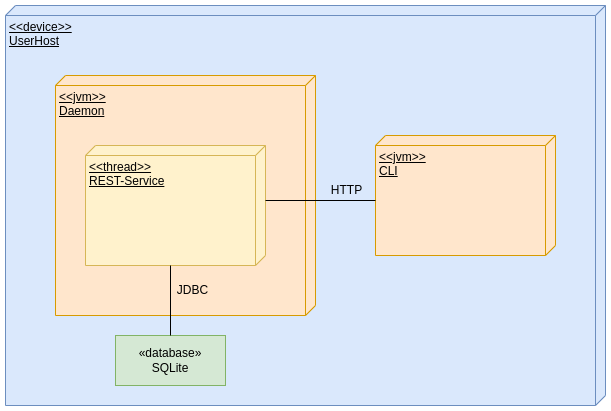
\includegraphics[width=1\textwidth]{assets/DeplDiagram-v2}
        \caption{UML Deploymentdiagramm}
        \label{fig:depl-diag}
    \end{figure}

    Das ganze System befindet sich während der Laufzeit auf dem Host-Gerät des Anwenders.
    Dazu werden zwei separate Jar-Dateien ausgeliefert.
    Die Erste sollte bereits beim Start des Geräts ausgeführt werden und die JVM für den Daemon starten.
    Dieser startet einen Webservice, der REST-Schnittstellen für die Steuerung des Daemons anbietet.
    Dieser REST-Service kommuniziert ausserdem über JDBC mit einem RDBMS, welches in Form von einer einzigen Datei (SQLite)
    in der Daemon-Applikation embedded ist.

    Das zweite Jar sollte dann manuell vom Anwender gestartet werden sobald er Funktionen des Daemons ausführen möchte.
    Dieses Jar startet wiederum eine zweite JVM, welche ein CLI für den Anwender mit bestimmten Kommandos zur Verfügung stellt.
    Diese CLI sendet dann über HTTP die entsprechenden Anfragen an den Daemon, die zur Erfüllung der Anweisungen des Anwenders führen.


    \section{Lizenzierung}
    Unser Projekt basiert auf den Prinzipien von \textbf{Free/Libre and Open Source Software (FLOSS)} und ist unter der \textbf{MIT-Lizenz} veröffentlicht.
    Diese Lizenz ermöglicht es, die Software frei zu nutzen, zu modifizieren und weiterzuverbreiten, sowohl für private als auch kommerzielle Zwecke, solange der ursprüngliche Lizenztext beibehalten wird.

    \subsection{Open-Source Abhängigkeiten}
    Im Projekt werden folgende Technologien und Bibliotheken verwendet, die ebenfalls unter Open-Source-Lizenzen stehen:

    \begin{itemize}
        \item \textbf{Java}: Entwickelt unter der \textbf{GPL v2 mit Classpath Exception}, was die Nutzung in geschlossenen Projekten ermöglicht.
        \item \textbf{Maven}: Unter der \textbf{Apache License 2.0}, die eine flexible Nutzung und Modifikation erlaubt.
        \item \textbf{Spring}: Ebenfalls lizenziert unter der \textbf{Apache License 2.0}, was eine Integration und Anpassung in eigenen Projekten ohne Einschränkungen unterstützt.
        \item \textbf{SQLite}: Steht unter der \textbf{Public Domain} bzw. der \textbf{blessing license}, wodurch es uneingeschränkt genutzt und verteilt werden kann.
        \item \textbf{H2}: Unter der \textbf{Mozilla Public License 2.0} (MPL 2.0), die flexible Nutzung, Modifikation und Distribution erlaubt, solange Änderungen am Quellcode unter derselben Lizenz veröffentlicht werden.
    \end{itemize}

    Durch die sorgfältige Auswahl dieser FLOSS-Lizenzen bleibt das Projekt vollständig mit den Open-Source-Grundsätzen kompatibel und bietet maximale Flexibilität für zukünftige Erweiterungen.

    \subsection{Kommerzielle Abhängigkeiten}
    Zusätzlich wird im Projekt ein kostenpflichtiger \textbf{GPT-Service} von \textit{OpenAI} eingebunden, der über eine API-Schnittstelle angebunden ist.
    Die Nutzung dieses Dienstes unterliegt den \textbf{kommerziellen Nutzungsbedingungen von OpenAI}.
    Es wird sichergestellt, dass der Zugriff auf diesen Dienst in unserem Projekt optional ist und die Kernfunktionalität auch ohne dessen Nutzung gewährleistet bleibt.
    Somit bleibt das Projekt als FLOSS klassifiziert, während die GPT-Integration als optionaler, externer Dienst gehandhabt wird.

    \clearpage


    \section{Installationshandbuch \& Skript}
    In diesem Kapitel sind die Installationsanleitungen für alle unterstützten Plattformen beschrieben.
    Grundsätzlich ist der TraceSentry ein plattformunabhängiges System, welches auf den gängigen Betriebssystemen (Windows, Linux, MacOS) lauffähig ist.
    Entwickelt und getestet wurde allerdings nur auf den folgenden Betriebssystemversionen, weshalb die Kompatibilität mit anderen Versionen nicht garantiert werden kann:
    \begin{itemize}
        \item Windows 11--10.0
        \item Linux 6.1.0-28
        \item macOS Sequoia 15.2
    \end{itemize}

    \textbf{Eine Installation der Java Laufzeitumgebung (JRE) wird für die Installation vorausgesetzt.}

    \subsection{Linux}\label{subsec:linux}
    \begin{enumerate}
        \item Durchsuchen Sie das neueste Artefakt, das vom Hauptbranch dieses Repositorys erstellt wurde, und laden Sie die Datei
        \texttt{target/tracesentry-\textless{}version\textgreater{}-submission.zip} auf Ihren Computer herunter.
        \item Entpacken Sie das Archiv in Ihr gewünschtes Installationsverzeichnis für TraceSentry.
        \item Definieren Sie die folgenden Umgebungsvariablen in der Datei \texttt{/etc/environment}:
        \begin{lstlisting}[label={lst:lstlisting-unix-1}]
JAVA_HOME=<absoluter Pfad zum JDK-Ordner>
TRACE_SENTRY_DIR=<absoluter Pfad zum Installationsverzeichnis>
        \end{lstlisting}
        Und fügen Sie die Variable \texttt{TRACE\_SENTRY\_DIR} am Ende der Datei \texttt{/etc/profile} zum \texttt{PATH} hinzu:
        \begin{lstlisting}[label={lst:lstlisting-unix-2}]
PATH=$PATH:$TRACE_SENTRY_DIR
        \end{lstlisting}
        \item Wenn Sie die Inspektionsfunktion nutzen möchten, erstellen Sie einen OpenAI-API-Schlüssel, indem Sie den Anweisungen unter \url{https://platform.openai.com/settings/organization/api-keys} folgen.
        Fügen Sie Guthaben zu Ihrem Konto hinzu, um die OpenAI-API nutzen zu können: \url{https://platform.openai.com/settings/organization/billing/overview}.
        Setzen Sie anschließend den generierten API-Schlüssel als Umgebungsvariable am Ende der Datei \texttt{/etc/profile}:
        \begin{lstlisting}[label={lst:lstlisting-unix-3}]
export OPENAI_API_KEY=<generierter API-Schlüssel>
        \end{lstlisting}
        Sollten Sie diesen Teil überspringen, werden Sie keinen Zugriff auf die Inspektionsfunktion haben.
        \item Wenn der Daemon\index{Daemon} bei jedem Systemstart automatisch im Hintergrund gestartet werden soll, können Sie Folgendes in einem Terminal ausführen:
        \begin{lstlisting}[label={lst:lstlisting-unix-4}]
crontab -e
// Fügen Sie die folgende Zeile am Ende der geöffneten Datei hinzu
@reboot PATH=$JAVA_HOME/bin:$PATH $TRACE_SENTRY_DIR/ts run
        \end{lstlisting}
        Speichern Sie dann die Datei.
        \item Nach einem Systemneustart sind Sie bereit, TraceSentry zu verwenden.
    \end{enumerate}

    \subsection{Windows}
    \begin{enumerate}
        \item Durchsuchen Sie das neueste Artefakt, das vom Hauptbranch dieses Repositorys erstellt wurde, und laden Sie die Datei
        \texttt{target/tracesentry-\textless{}version\textgreater{}-submission.zip} auf Ihren Computer herunter.
        \item Entpacken Sie das Archiv in Ihr gewünschtes Installationsverzeichnis für TraceSentry.
        \item Setzen Sie die Umgebungsvariable \texttt{TRACE\_SENTRY\_DIR} via Systemsteuerung oder via PowerShell:
        \begin{lstlisting}[label={lst:lstlisting-windows-1}]
[System.Environment]::SetEnvironmentVariable("TRACE_SENTRY_DIR", "<absoluter Pfad zum Installationsverzeichnis>","User")
        \end{lstlisting}
        \item Damit die CLI korrekt funktioniert, fügen Sie das Installationsverzeichnis zum \texttt{PATH} hinzu:
        \begin{lstlisting}[label={lst:lstlisting-windows-2}]
$currentPath = [System.Environment]::GetEnvironmentVariable("Path", "User")
[System.Environment]::SetEnvironmentVariable("Path", "$currentPath;<absoluter Pfad zum Installationsverzeichnis>","User")
        \end{lstlisting}
        \item Wenn Sie die Inspektionsfunktion nutzen möchten, erstellen Sie einen OpenAI-API-Schlüssel, indem Sie den Anweisungen unter \url{https://platform.openai.com/settings/organization/api-keys} folgen.
        Fügen Sie Guthaben zu Ihrem Konto hinzu, um die OpenAI-API nutzen zu können: \url{https://platform.openai.com/settings/organization/billing/overview}.
        Setzen Sie anschließend den generierten API-Schlüssel als Umgebungsvariable via PowerShell:
        \begin{lstlisting}[label={lst:lstlisting-windows-3}]
[System.Environment]::SetEnvironmentVariable("OPENAI_API_KEY", "<generierter API-Schluessel>","User")
        \end{lstlisting}
        Sollten Sie diesen Teil überspringen, werden Sie keinen Zugriff auf die Inspektionsfunktion haben.
        \item Wenn der Daemon\index{Daemon} bei jedem Systemstart automatisch im Hintergrund gestartet werden soll, muss die Datei \texttt{ts-daemon.bat} vom Installationsverzeichnis in den Autostart-Ordner kopiert werden:
        \begin{lstlisting}[label={lst:lstlisting-windows-4}]
Copy-Item "$env:TRACE_SENTRY_DIR\ts-daemon.bat" "$env:APPDATA\Microsoft\Windows\Start Menu\Programs\Startup"
        \end{lstlisting}
        Beim nächsten Systemstart wird der Daemon automatisch gestartet.
        Beim ersten Start kann eine Sicherheitswarnung erscheinen, in der Sie eine Checkbox deaktivieren müssen, damit diese in Zukunft nicht mehr erscheint.
        \item Starten Sie das Terminal neu, und Sie sind bereit, TraceSentry zu verwenden.
    \end{enumerate}

    \clearpage

    \subsection{macOS}\label{subsec:macos}
    Der Einfachheit halber werden hier ausschliesslich Konfigurationen im \texttt{.zprofile} File benützt.
    Die nachfolgenden Befehle schreiben die Konfigurationen direkt in die Datei.
    \begin{enumerate}
        \item Durchsuchen Sie das neueste Artefakt, das vom Hauptbranch dieses Repositorys erstellt wurde, und laden Sie die Datei
        \texttt{target/tracesentry-\textless{}version\textgreater{}-submission.zip} auf Ihren Computer herunter.
        \item Entpacken Sie das Archiv in Ihr gewünschtes Installationsverzeichnis für TraceSentry.
        \item Setzen Sie die Umgebungsvariable \texttt{TRACE\_SENTRY\_DIR} im \texttt{.zprofile} File (befindet sich in Ihrem Home-Verzeichnis):
        \begin{lstlisting}[label={lst:lstlisting-mac-1}]
echo '\n# Added for TraceSentry' >> ~/.zprofile
echo export TRACE_SENTRY_DIR="<absoluter Pfad zum Installationsverzeichnis>" >> ~/.zprofile
        \end{lstlisting}
        \item Damit die CLI korrekt funktioniert, fügen Sie im \texttt{.zprofile} File das Installationsverzeichnis zum \texttt{PATH} hinzu:
        \begin{lstlisting}[label={lst:lstlisting-mac-2}]
echo export PATH="\$TRACE_SENTRY_DIR:\$PATH" >> ~/.zprofile
        \end{lstlisting}
        \item Wenn Sie die Inspektionsfunktion nutzen möchten, erstellen Sie einen OpenAI-API-Schlüssel, indem Sie den Anweisungen unter \url{https://platform.openai.com/settings/organization/api-keys} folgen.
        Fügen Sie Guthaben zu Ihrem Konto hinzu, um die OpenAI-API nutzen zu können: \url{https://platform.openai.com/settings/organization/billing/overview}.
        Setzen Sie anschließend den generierten API-Schlüssel als Umgebungsvariable im \texttt{.zprofile} File:
        \begin{lstlisting}[label={lst:lstlisting-mac-3}]
echo export OPENAI_API_KEY=<generierter API-Schluessel> >> ~/.zprofile
        \end{lstlisting}
        Sollten Sie diesen Teil überspringen, werden Sie keinen Zugriff auf die Inspektionsfunktion haben.
        \item Wenn der Daemon\index{Daemon} bei jedem Systemstart automatisch im Hintergrund gestartet werden soll, passen Sie das \texttt{.zprofile} File in ihrem Home-Verzeichnis wie folgt an:
        \begin{lstlisting}[label={lst:lstlisting-mac-4}]
echo ts run >> ~/.zprofile
        \end{lstlisting}
        Dies wird als pragmatische Lösung empfohlen.
        Alternativ können Sie auch \textit{launchd} verwenden. \cite{appleDeveloper}
        \item Starten Sie das Terminal neu, dadurch wird der Daemon automatisch gestartet (sofern Sie Schritt 6 befolgt haben), und Sie sind bereit, TraceSentry zu verwenden.
    \end{enumerate}

    \clearpage


    \section{Benutzerhandbuch}
    \label{sec:user-manual}
    In diesem Abschnitt soll der Nutzer eine Anleitung für die Verwendung des TraceSentry-Systems erhalten.
    Dazu hier der Verweis auf die CLI-Dokumentation im Anhang~\ref{sec:cli-doc}.
    \\
    Vorab noch einige Hinweise zur Verwendung des Systems:
    \begin{itemize}
        \item Der TraceSentry kann sowohl im interaktiven Modus, sowie auch im nicht-interaktiven Modus verwendet werden.
        Der Unterschied besteht darin, dass beim interaktiven Modus zu Beginn ein einziges Mal die CLI mit einer neuen Session gestartet wird und
        dann alle folgenden Befehle in dieser Session/Laufzeit ausgeführt werden.
        Dieser interaktive Modus wird gestartet, indem in einem Host-Terminal nur der Befehl \texttt{ts} ausgeführt wird.
        Hingegen wird beim nicht-interaktiven Modus die gesamte CLI-Applikation bei jedem Befehl neu gestartet und nach dessen beendeter Ausführung auch direkt wieder beendet.
        Der nicht-interaktive Modus wird gestartet, indem in einem Host-Terminal der Befehl \texttt{ts <Befehl>} ausgeführt wird.
        \item Im TraceSentry ist ein \texttt{help}-Befehl eingebaut, welcher eine Übersicht über alle verfügbaren Befehle und deren Verwendung anzeigt.
        Dieser Befehl wird genau gleich wie alle anderen Befehle ausgeführt, indem im Host-Terminal \texttt{ts help} eingegeben wird.
        Um genauere Informationen zu einem bestimmten Befehl des TraceSentry's zu erhalten kann nach dem \texttt{help}-Befehl auch der Name des gewünschten Befehls angegeben werden (z.B. \texttt{ts help monitor}).
        \item Für die Verwendung mit \textbf{Windows} ist zu beachten, dass alle Pfade in den Befehlen mit \textbf{zwei} Backslash (\textbackslash) geschrieben werden müssen.
        \item Pfade welche Leerzeichen enthalten, müssen in Anführungszeichen gesetzt werden.
    \end{itemize}


    \chapter{Fazit}


    \section{Diskussion}
    Das Projekt hat die Relevanz der Problematik im Umgang mit Cache- und Log-Dateien aufgezeigt und eine erste Lösung erarbeitet, mit der ein Anwender die Integrität dieser Dateien überwachen kann.
    Die Nutzung von generativen KI-Modellen zur Analyse von solchen Dateien hat sich dabei als effektives Mittel erwiesen, um Anomalien zu erkennen und einzuordnen.

    Die Verwendung ebendieser KI-Modelle regt aber auch neue Diskussionen an, insbesondere im Hinblick auf den Datenschutz und die Privatsphäre.
    Denkt man an das Kernproblem - dem Schutz von sensiblen Daten - so ist die Verwendung eines kommerziellen und proprietären KI-Modells wie es die GPT-Modelle sind, durchaus kritisch zu betrachten
    und regt im Grunde das selbe Problem an, das sie eigentlich lösen sollte.

    Des Weiteren ist die umgesetzte Lösung mit der Kommandozeilenschnittstelle vor allem für technisch versierte Anwender geeignet.
    Diese haben zwar auch Bedarf an einer solchen Lösung, jedoch sind sie eher in der Lage, auch ohne ein solches Tool die Risiken einzuschätzen und zu minimieren.
    Gerade für weniger technische versierte Anwender, die oft nicht in der Lage sind, die Risiken zu erkennen und zu minimieren, wäre eine einfache und intuitive Lösung umso wichtiger.

    Für eine zukünftige Weiterentwicklung könnten neben der besagten UX-Verbesserung etliche Funktionen und technische Verbesserungen vorgenommen werden.
    Das Problem bietet sehr viel Raum dafür.

    Nichtsdestotrotz ist die Lösung in ihrer jetzigen Form ein Anfang, löst das ursprüngliche Problem und bietet eine Basis, auf der weiter aufgebaut werden kann.
    Die Arbeit bietet zudem die Möglichkeit, das Potential von generativen KI-Modellen für spezifische Anwendungsfälle zu erkennen und ein Verständnis zu schaffen, wie diese in Zukunft eingesetzt werden können.

    \clearpage


    \section{Endergebnis}\label{sec:endergebnis}
    Im Verlauf des Projekts wurde eine Software entwickelt, die es ermöglicht, jegliche Art von Dateien zu suchen, zu überwachen und zu löschen.
    Dabei bietet das System direkt die Möglichkeit dies für Cache- und Log-Dateien zu tun.
    Mittels angebundenem KI-Modell, können schnell und effizient Einschätzungen zu solchen Dateien eingeholt werden und so potentielle Gefahren erkannt und eine Löschung veranlasst werden.

    Es wurde ein FLOSS lizenziertes und plattformunabhängiges System entwickelt, das auf eine CLI- und Daemon-Architektur setzt und auf dem Host des Anwenders installiert und ausgeführt wird.
    In der jetzigen Form richtet es sich an eine Zielgruppe, zwischen Laien und Experten, vor allem in der Hinsicht der Kommandozeilenschnittstelle.

    Während die praktische Umsetzung der Software die grundlegenden Anforderungen erfüllt, hat das Projekt zudem die Chancen und Grenzen von generativen KI-Modellen in einer Fallstudie aufgezeigt.

    Die primäre Zielsetzung wurde erreicht und das Erweiterungspotential wird im folgenden Kapitel diskutiert.

    \subsection{Berechnung der Produktivitätssteigerung}\label{subsec:berechnung-der-produktivitatssteigerung}
    In diesem Abschnitt wird die geschätzte Produktivitätssteigerung für Benutzer von \\TraceSentry berechnet.
    Die Berechnungsfaktoren umfassen die \textbf{Aufgabendauer ohne und mit der Software}, die resultierende  \textbf{Zeitersparnis}, die  \textbf{Kosten pro Zeiteinheit} und die  \textbf{Gesamtkostenersparnis}.

    Die folgenden Befehle sind in der~\nameref{sec:cli-doc} spezifiziert.
    \\Es wird das \texttt{inspect} Kommando und die Monitoring-Funktionen betrachtet.
    Für Funktionen wie \texttt{search} und \texttt{wipe} wird keine Produktivitätssteigerung angenommen, da sie nur Shell-Befehle umhüllen.
    Administrationsbefehle wie \texttt{kill}, \texttt{run} etc.\ werden ebenfalls nicht betrachtet, diese sind \("\)Mittel zum Zweck\("\) und es gibt logischerweise keine äquivalenten Vorgänge ohne die Software.

    \clearpage

    \subsubsection{Berechnung}

    \paragraph*{Annahmen}
    Für die Berechnung der Produktivitätssteigerung werden folgende Annahmen getroffen:
    \begin{itemize}
        \item TraceSentry ist gemäss Installationshandbuch installiert (inkl.\ Autostart).
        \item Das Hochladen einer Datei in die GPT-Prompt dauert inkl.\ dem Vorschlagen der Output-Formulierung bzw.\ -Formatierung ca.\ 20 Sekunden.
        \item Die Analyse einer Datei in der GPT-Prompt dauert ca.\ 5 Sekunden.
        \item TraceSentry benötigt im Schnitt 4 Sekunden für das \texttt{inspect} Kommando (für eine beliebige Datei).
        \item Der durchschnittliche Studenlohn beträgt 38 CHF\@.
        \item Eine Datei wird im Schnitt für eine Woche überwacht.
        \item Ein Computer läuft im Schnitt 6 Stunden pro Tag.
        \item TraceSentry benötigt im Schnitt 600ms für das Erstellen eines Snapshots.
        \item Das Erstellen einer Kopie einer Datei (manueller Snapshot) dauert ca.\ 10 Sekunden.
        \item Das Vergleichen zweier Dateien dauert ca.\ 20 Sekunden.
    \end{itemize}

    \clearpage

    Texte als Variablen sind folgend als Zeitdauer zu verstehen. \\

    \textbf{Analyse \texttt{inspect} Funktion} \\

    \textbf{Ohne TraceSentry:} \\
    \begin{align*}
        \text{Input vorbereiten}&: \text{Dateiinhalt in GPT-Prompt kopieren/hochladen}\\
        \text{Output abwarten}&: \text{GPT-Response} \\
        \text{Aufgabendauer ohne SW} &= \text{(Input vorbereiten + Output abwarten)} \\
        &= 20s + 5s \\
        &= 25s \\
    \end{align*}

    \text{\textbf{Mit TraceSentry:}} \\
    \begin{align*}
        \text{Aufgabendauer mit SW} &= \text{\texttt{inspect}} \\
        &= 4s
    \end{align*}

    \text{\textbf{Produktivitätssteigerung:}} \\
    \begin{align*}
        \text{Zeitersparnis} &= 25 - 4 = 21s = 0.35min \\
        \text{Kosten pro Zeiteinheit} &= 38 \text{CHF/Stunde} \\ &\approx 0.63 \text{CHF/Minute} \\
        \text{Gesamtkostenersparnis} &= 0.35 * 0.63 \text{CHF/Minute} \\ &= 0.2205 \text{ CHF} \\ &= 22.05 \text{ Rappen (pro Datei)} \\
        \\
        \text{Produktivitätssteigerung} &= \frac{\text{Zeitersparnis}}{\text{Aufgabendauer ohne SW}}
        \\ &= \frac{\text{21}}{\text{25}}
        \\ &= 84\%
    \end{align*}

    \newpage

    \textbf{Analyse Monitoring Funktion} \\

    \textbf{Ohne TraceSentry:} \\
    \\

    Erläuterung: Der Benutzer speichert hierbei für eine Woche, 6 Mal am Tag manuell die Datei (als Snapshot) in einen dafür vorgesehenen Ordner.
    \begin{align*}
        \text{Manueller Snapshot erstellen}&: \text{Datei in einen Ordner speichern}\\
        \text{Snapshots vergleichen}&: \text{zwei aufeinander folgende Snapshots vergleichen} \\
        \text{Aufgabendauer ohne SW} &= \text{6 * 7 * (Manueller Snapshot erstellen + Snapshots vergleichen)} \\
        &= 6 * 7 * (10s + 20s) \\
        &= 1260s \\
        &= 21min \\
    \end{align*}

    \textbf{Mit TraceSentry:} \\
    \begin{align*}
        \text{Aufgabendauer mit SW} &= \text{6 * 7 * Snapshot erstellen} \\
        &= 6 * 7 * 600ms \\
        &= 25200ms \\
        &\approx 25s \\
    \end{align*}

    \text{\textbf{Produktivitätssteigerung:}} \\
    \begin{align*}
        \text{Zeitersparnis} &= 1260 - 25 = 1235s \\
        &\approx 20.58min \\
        \text{Kosten pro Zeiteinheit} &= 38 \text{CHF/Stunde} \\ &\approx 0.63 \text{CHF/Minute} \\
        \text{Gesamtkostenersparnis} &= 20.58 * 0.63 \text{CHF/Minute} \\ &= 12.9654 \text{ CHF (pro überwachte Datei)} \\
        \\
        \text{Produktivitätssteigerung} &= \frac{\text{Zeitersparnis}}{\text{Aufgabendauer ohne SW}}
        \\ &= \frac{\text{1235}}{\text{1260}}
        \\ &\approx 98\%
    \end{align*}


    \clearpage


    \section{Zukünftige Arbeiten}\label{sec:zukunftigearbeiten}

    \subsection{Funktionale Erweiterungen}\label{subsec:funktionale-erweiterungen}

    \subsubsection{Ideen aus der Originalen Projektbeschreibung}
    Folgende Features können dem Proposal (\nameref{sec:originale-projektbeschreibung}) entnommen werden.
    Teilweise wurden diese nicht vollständig umgesetzt.
    Dies hängt mit der generellen Philosophie der realisierten Lösung, sowie Gründen der Zeit und Komplexität zusammen.
    \begin{itemize}
        \item \textbf{Schlüsse aus Änderungen ziehen\footnotemark[1]}: Die Abfrage des KI-Modells könnte erweitert werden, um nicht nur Dateiinhalte zu analysieren, sondern auch Schlüsse aus Änderungen, Löschungen und Neuerstellungen von Dateimetadaten und/oder Dateiinhalten zu ziehen.
        \item \textbf{Detektion von unautorisiertem Schreibzugriff \footnotemark[1]}: Das System könnte erweitert werden, um unautorisierte Schreibzugriffe auf Dateien zu erkennen, einzuordnen und zu verhindern.
    \end{itemize}

    \subsubsection{Generelle Ideen für zukünftige Features}
    \begin{itemize}
        \item \textbf{Individuelle Monitoring Intervalle}: Der Anwender soll die Möglichkeit haben, die Periodizität des Monitorings pro überwachter Datei individuell einzustellen.
        \item \textbf{Monitoring von geschützten Verzeichnissen/Dateien}: Der Anwender soll die Möglichkeit haben (eventuell mit Erfordernissen via Betriebssystems), geschützte Verzeichnisse/Dateien zu überwachen.
        \item \textbf{Doppel-Backslash in Windows}: Wegen des Escapings von Java sind momentan in Windows-Pfaden doppelte Backslashes notwendig.
        Dies könnte mit einer Erweiterung im \texttt{ts.bat} Skript für Windows behoben werden.
    \end{itemize}

    \footnotetext[1]{Gemäss
    \nameref{sec:originale-projektbeschreibung}:
        \begin{quote}
            any sense of it being wiped or even deleted (and its recreation
            being prohibited through file access rights, which - en passant - may enable the
            detection of any unauthorised file writer)
        \end{quote}}

    \subsection{User Experience}\label{subsec:user-experience}
    Der generelle technische Aufbau des Systems und insbesondere dessen Architektur bieten die Möglichkeit zusätzliche Clients zu entwickeln.
    Insbesondere eine grafische Benutzeroberfläche (GUI) könnte die Benutzerfreundlichkeit des Systems erheblich verbessern und die Zielgruppe erweitern.
    Die REST-Schnittstelle des Daemons bietet die notwendige Flexibilität dafür.

    In Belangen der Benutzerfreundlichkeit wäre ausserdem eine Verbesserung der Fehlermeldungen (mit besserem Exceptionhandling) in Betracht zu ziehen.

    \clearpage

    \subsection{Sicherheit}\label{subsec:sicherheit}
    In der jetzigen Lösung wurde wenig bis gar keine Rücksicht auf Sicherheitsaspekte genommen.
    Das deshalb, weil das System als Ganzes nur auf dem Host des Anwenders läuft und keine externen Schnittstellen bietet.
    Es sind also primär Angriffe \("\)von innen\("\) möglich.
    Dabei ist vor allem die ungesicherte REST-Schnittstelle des Daemons anfällig.
    Das Hinzufügen von Authentifizierung und Autorisierung (v.a.\ der REST-Schnittstelle), wäre also ein wichtiger Schritt in einer zukünftigen Version.

    \subsection{Erweiterung der KI-Modelle bzw. Anbindung}\label{subsec:erweiterung-der-ki-modelle}
    Im Rahmen dieser Arbeit wurde nur ein einziges KI-Modell (GPT-4o mini) eingebunden.
    Dieses ist, obwohl nicht primär dafür entwickelt, durchaus in der Lage, die Anforderungen des TraceSentry zu erfüllen.
    In einer zukünftigen Version könnte die Anbindung von weiteren Modellen, die spezifisch für Anomalieerkennung in Dateien entwickelt wurden, in Betracht gezogen werden.
    Falls notwendig, könnte auch ein eigenes Modell entwickelt werden.

    \subsection{Dateikompatibilität}\label{subsec:dateikompatibilitat}
    Bei der Inspektion von Dateien durch KI sowie dem Erstellen eines Merkle-Trees für die periodische Überwachung wird jeweils der gesamte Dateiinhalt via Java Files-API eingelesen.
    Dies Funktion \texttt{readAllBytes} hat dabei eine Limitierung von 2 GB pro Datei~\cite{javaAPI}.
    Hierbei könnte man in einer zukünftigen Version die Dateien für die Inspektion in kleinere Teile aufteilen und diese separat analysieren.
    Für die Erstellung des Merkle-Trees wäre ein möglicher Ansatz, die Dateien in Blöcke von 2 GB zu teilen und diese einzeln zu hashen.
    Die Hashes aller Blöcke könnten dann konkateniert und gehasht werden, um den Hash-Wert der gesamten Datei zu erhalten.

    %------------ Glossary -------------------
    \addcontentsline{toc}{chapter}{Glossar}
    \printglossary

    %------------ Index ----------------------
    \clearpage
    \printindex

    %----------- Bibliography ----------
    %------
    \clearpage
    \begin{thebibliography}{99}

        \bibitem{javaAPI}
        Oracle.
        \textit{Java Files-API Dokumentation: \url{https://docs.oracle.com/javase/8/docs/api/java/nio/file/Files.html\#readAllBytes-java.nio.file.Path-}}.
        Zuletzt aufgerufen am 10. Januar 2025.

        \bibitem{appleDeveloper}
        Developer Apple.
        \textit{Creating Launchd Jobs}.
        \url{https://developer.apple.com/library/archive/documentation/MacOSX/Conceptual/BPSystemStartup/Chapters/CreatingLaunchdJobs.html}, zuletzt aufgerufen am 10. Januar 2025.


        \bibitem{geeksforgeeks2025}
        GeeksforGeeks.
        \textit{Introduction to Merkle Tree}.
        \url{https://www.geeksforgeeks.org/introduction-to-merkle-tree/}, zuletzt aufgerufen am 10. Januar 2025.

        \bibitem{wikipedia2025}
        Wikipedia.
        \textit{Merkle Tree}.
        \url{https://en.wikipedia.org/wiki/Merkle_tree}, zuletzt aufgerufen am 10. Januar 2025.

        \bibitem{baeldung2025}
        Baeldung.
        \textit{Merkle Trees}.
        \url{https://www.baeldung.com/cs/merkle-trees}, zuletzt aufgerufen am 10. Januar 2025.

        \bibitem{spring2025}
        Spring Framework.
        \textit{Spring Shell - Getting Started}.
        \url{https://docs.spring.io/spring-shell/reference/3.3/getting-started.html}, zuletzt aufgerufen am 10. Januar 2025.

        \bibitem{mckinsey2025}
        McKinsey \& Company.
        \textit{The Economic Potential of Generative AI: The Next Productivity Frontier}.
        \url{https://www.mckinsey.com/capabilities/mckinsey-digital/our-insights/the-economic-potential-of-generative-ai-the-next-productivity-frontier}, zuletzt aufgerufen am 10. Januar 2025.

        \bibitem{openai2025}
        OpenAI\@.
        \textit{Models Documentation}.
        \url{https://platform.openai.com/docs/models}, zuletzt aufgerufen am 10. Januar 2025.

    \end{thebibliography}

    %------------ Appendix ----------------
    \appendix


    \chapter{Anhang}
    \clearpage

    \vspace*{\fill}
    \thispagestyle{empty}
    \titleformat{\section}{\centering\normalfont\Large\bfseries}{\thesection}{1em}{}


    \section{Originale Projektbeschreibung}\label{sec:originale-projektbeschreibung}
    \vspace*{\fill}
    
\includepdf[pages=-]{../misc/proposal.pdf}


    \vspace*{\fill}
    \thispagestyle{empty}
    \titleformat{\section}{\centering\normalfont\Large\bfseries}{\thesection}{1em}{}


    \section{CLI Dokumentation}\label{sec:cli-doc}\index{CLI}
    \vspace*{\fill}
    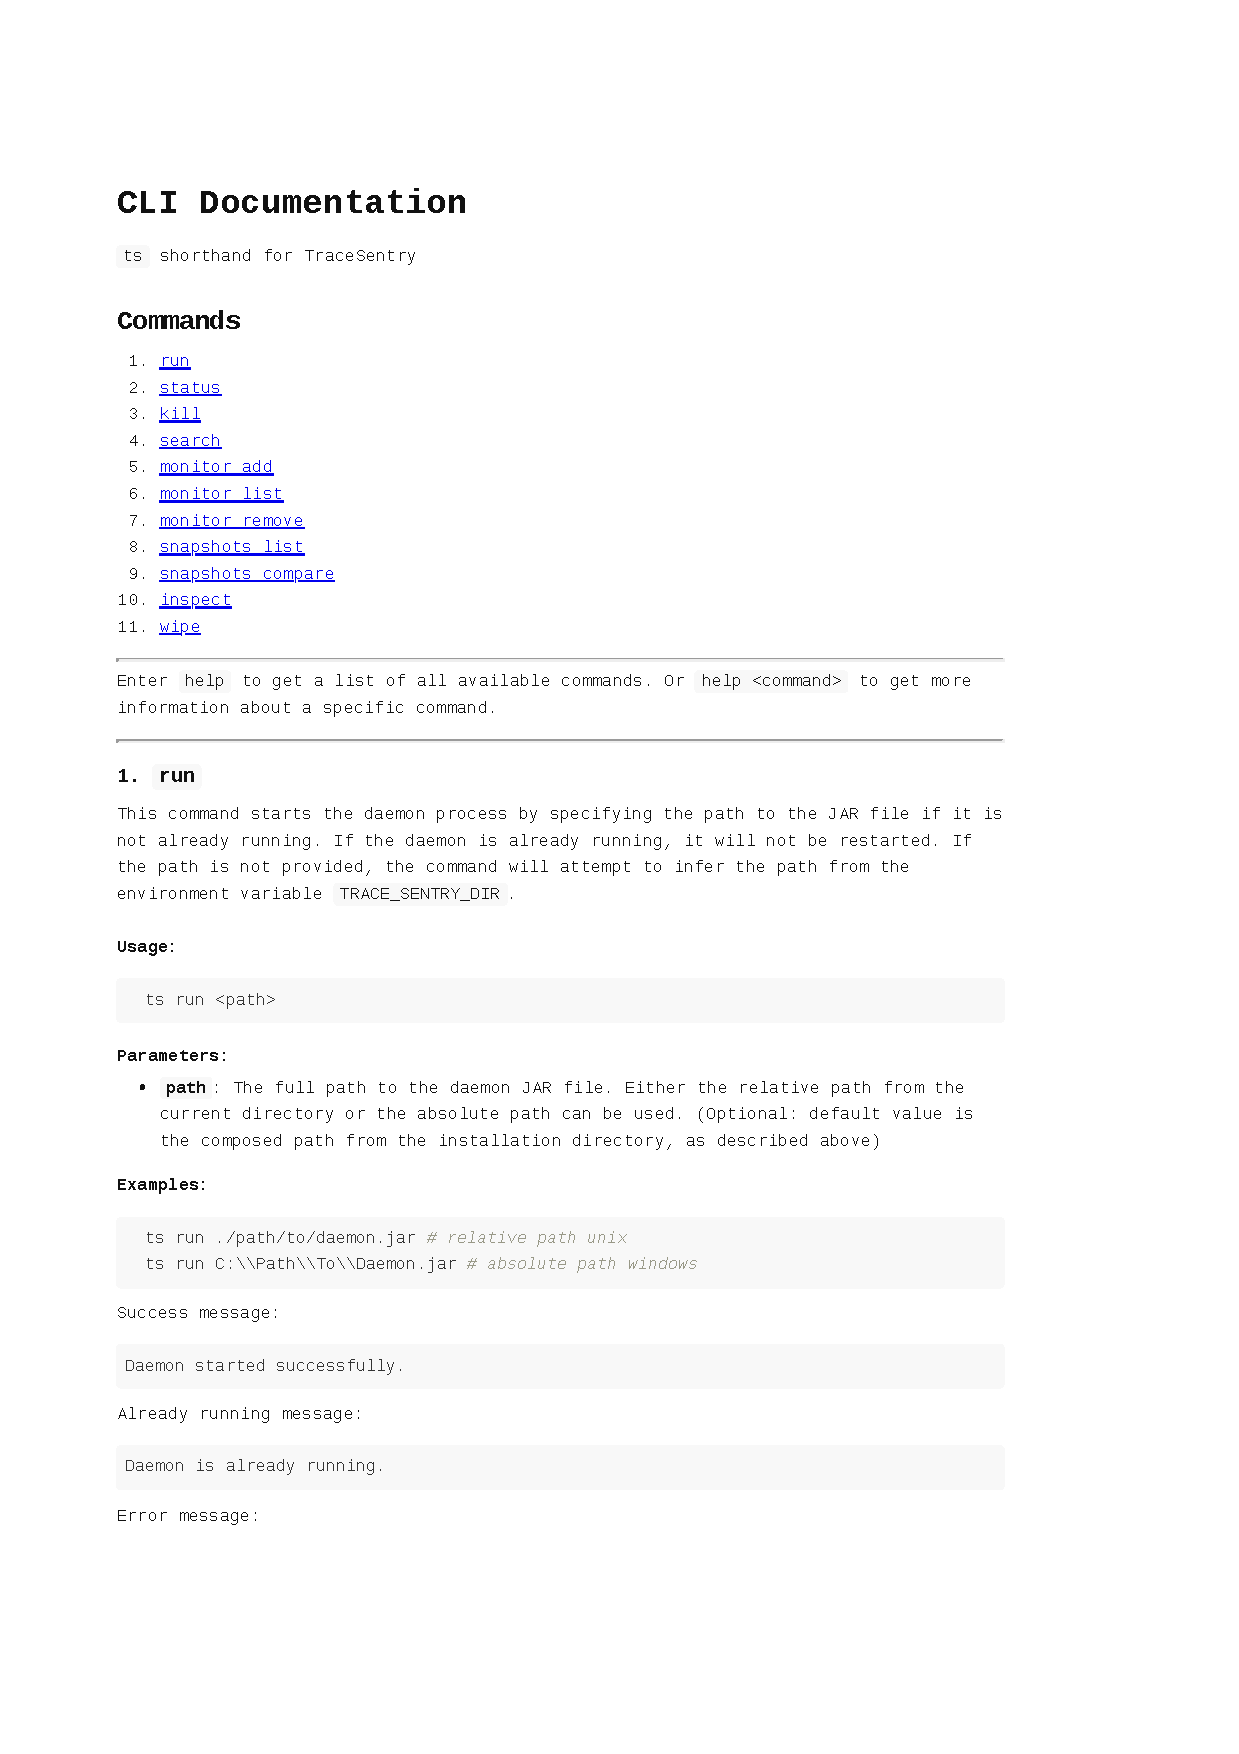
\includepdf[pages=-]{assets/cli-doc.pdf}

    \vspace*{\fill}
    \thispagestyle{empty}
    \titleformat{\section}{\centering\normalfont\Large\bfseries}{\thesection}{1em}{}


    \section{API-Dokumentation}\label{sec:api-spec}\index{REST-API}
    \vspace*{\fill}
    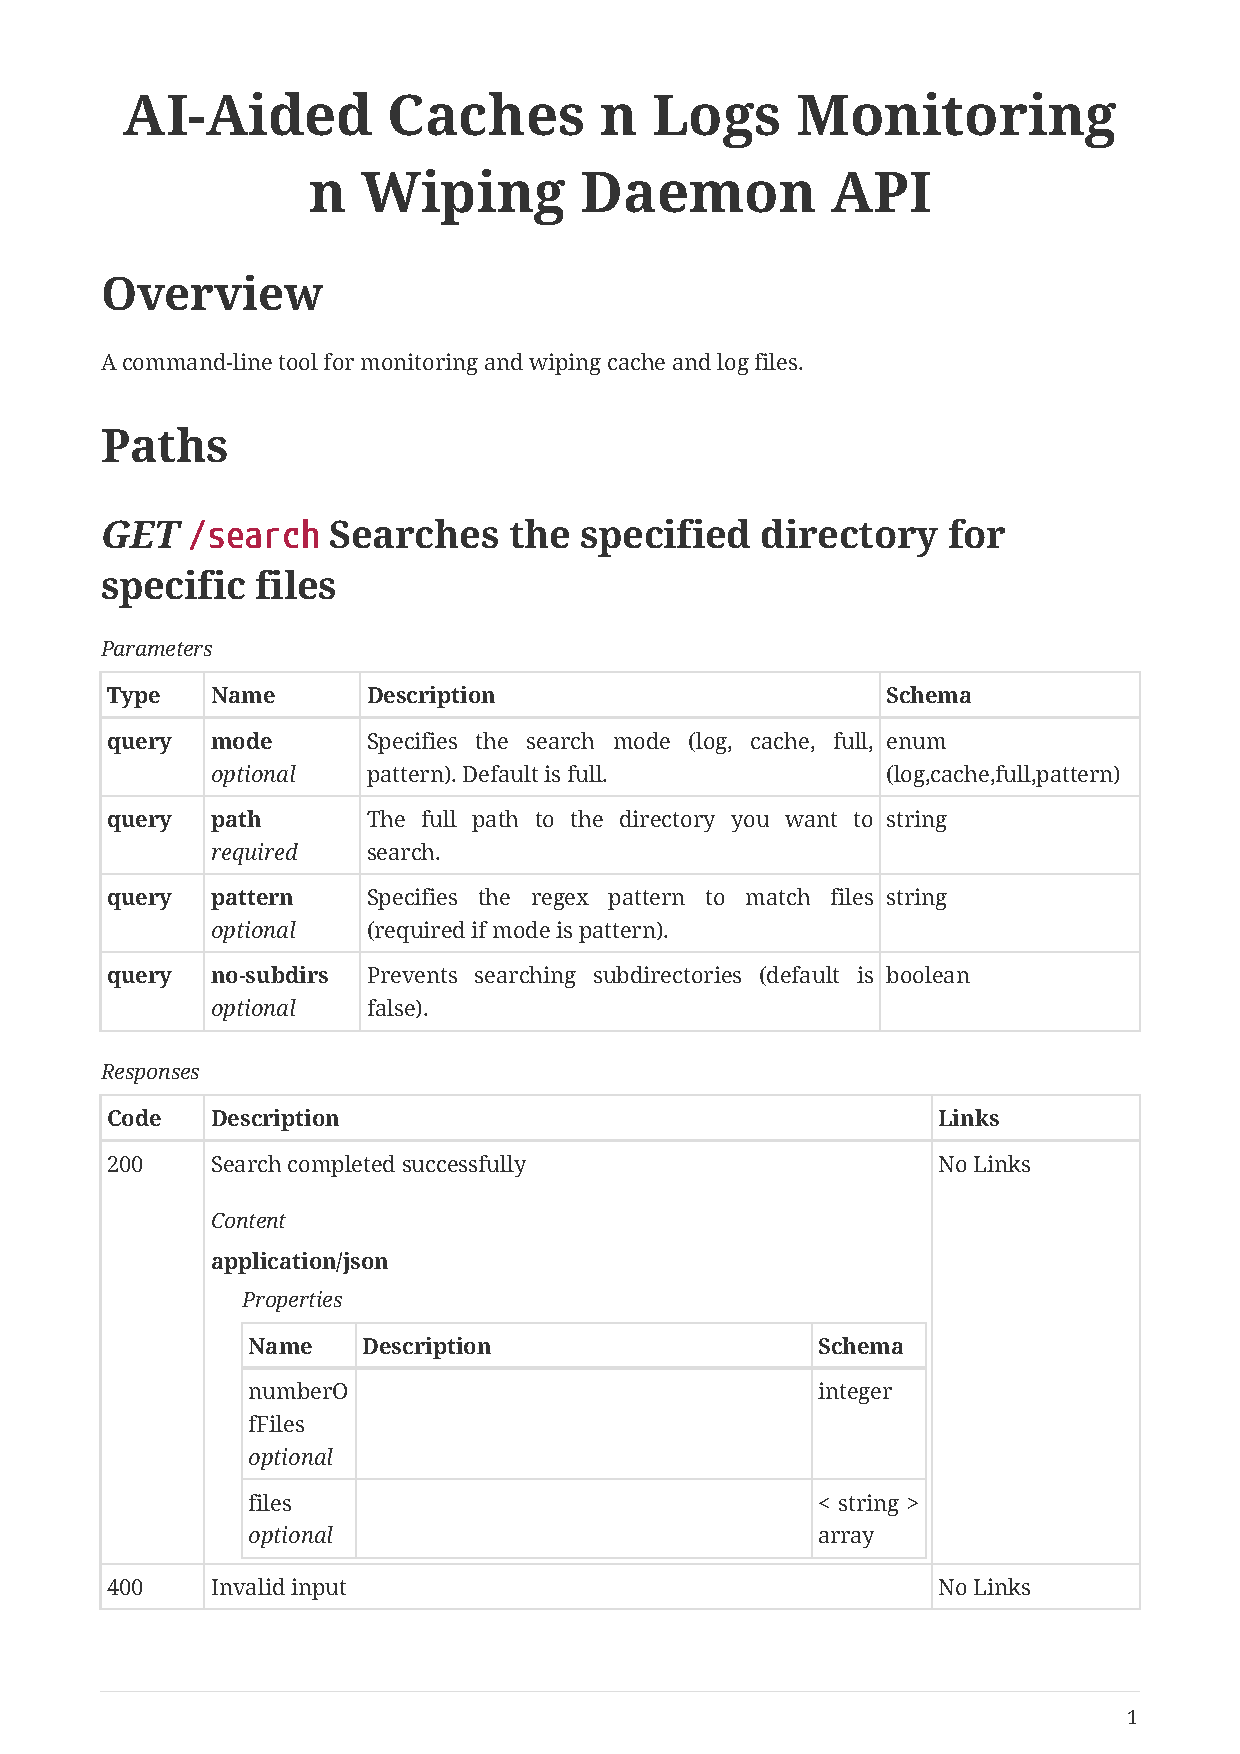
\includepdf[pages=-]{assets/api-documentation.pdf}

    \vspace*{\fill}
    \thispagestyle{empty}
    \titleformat{\section}{\centering\normalfont\Large\bfseries}{\thesection}{1em}{}


    \section{Klassendiagramm CLI}
    \label{sec:class-diag-cli}

    \begingroup
    \renewcommand{\thefootnote}{\roman{footnote}}
    \footnotetext[0]{
        \begin{itemize}
            \item Falls das Diagramm nicht optimal dargestellt wird, kann es im Abgabeordner unter folgenden Pfaden gefunden werden:
            \texttt{docs/diagrams/intellij/cli.uml} (kann nur mit IntelliJ IDEA geöffnet werden) bzw. \texttt{docs/assets/cli\_class\_diag.png}
            \item Wegen dem Spring IoC Container: nicht alle Beziehungen zwischen Klassen abgebildet.
            \item Diagramm erstellt mit IntelliJ IDEA Ultimate.
        \end{itemize}
    }
    \endgroup

    \vspace*{\fill}
    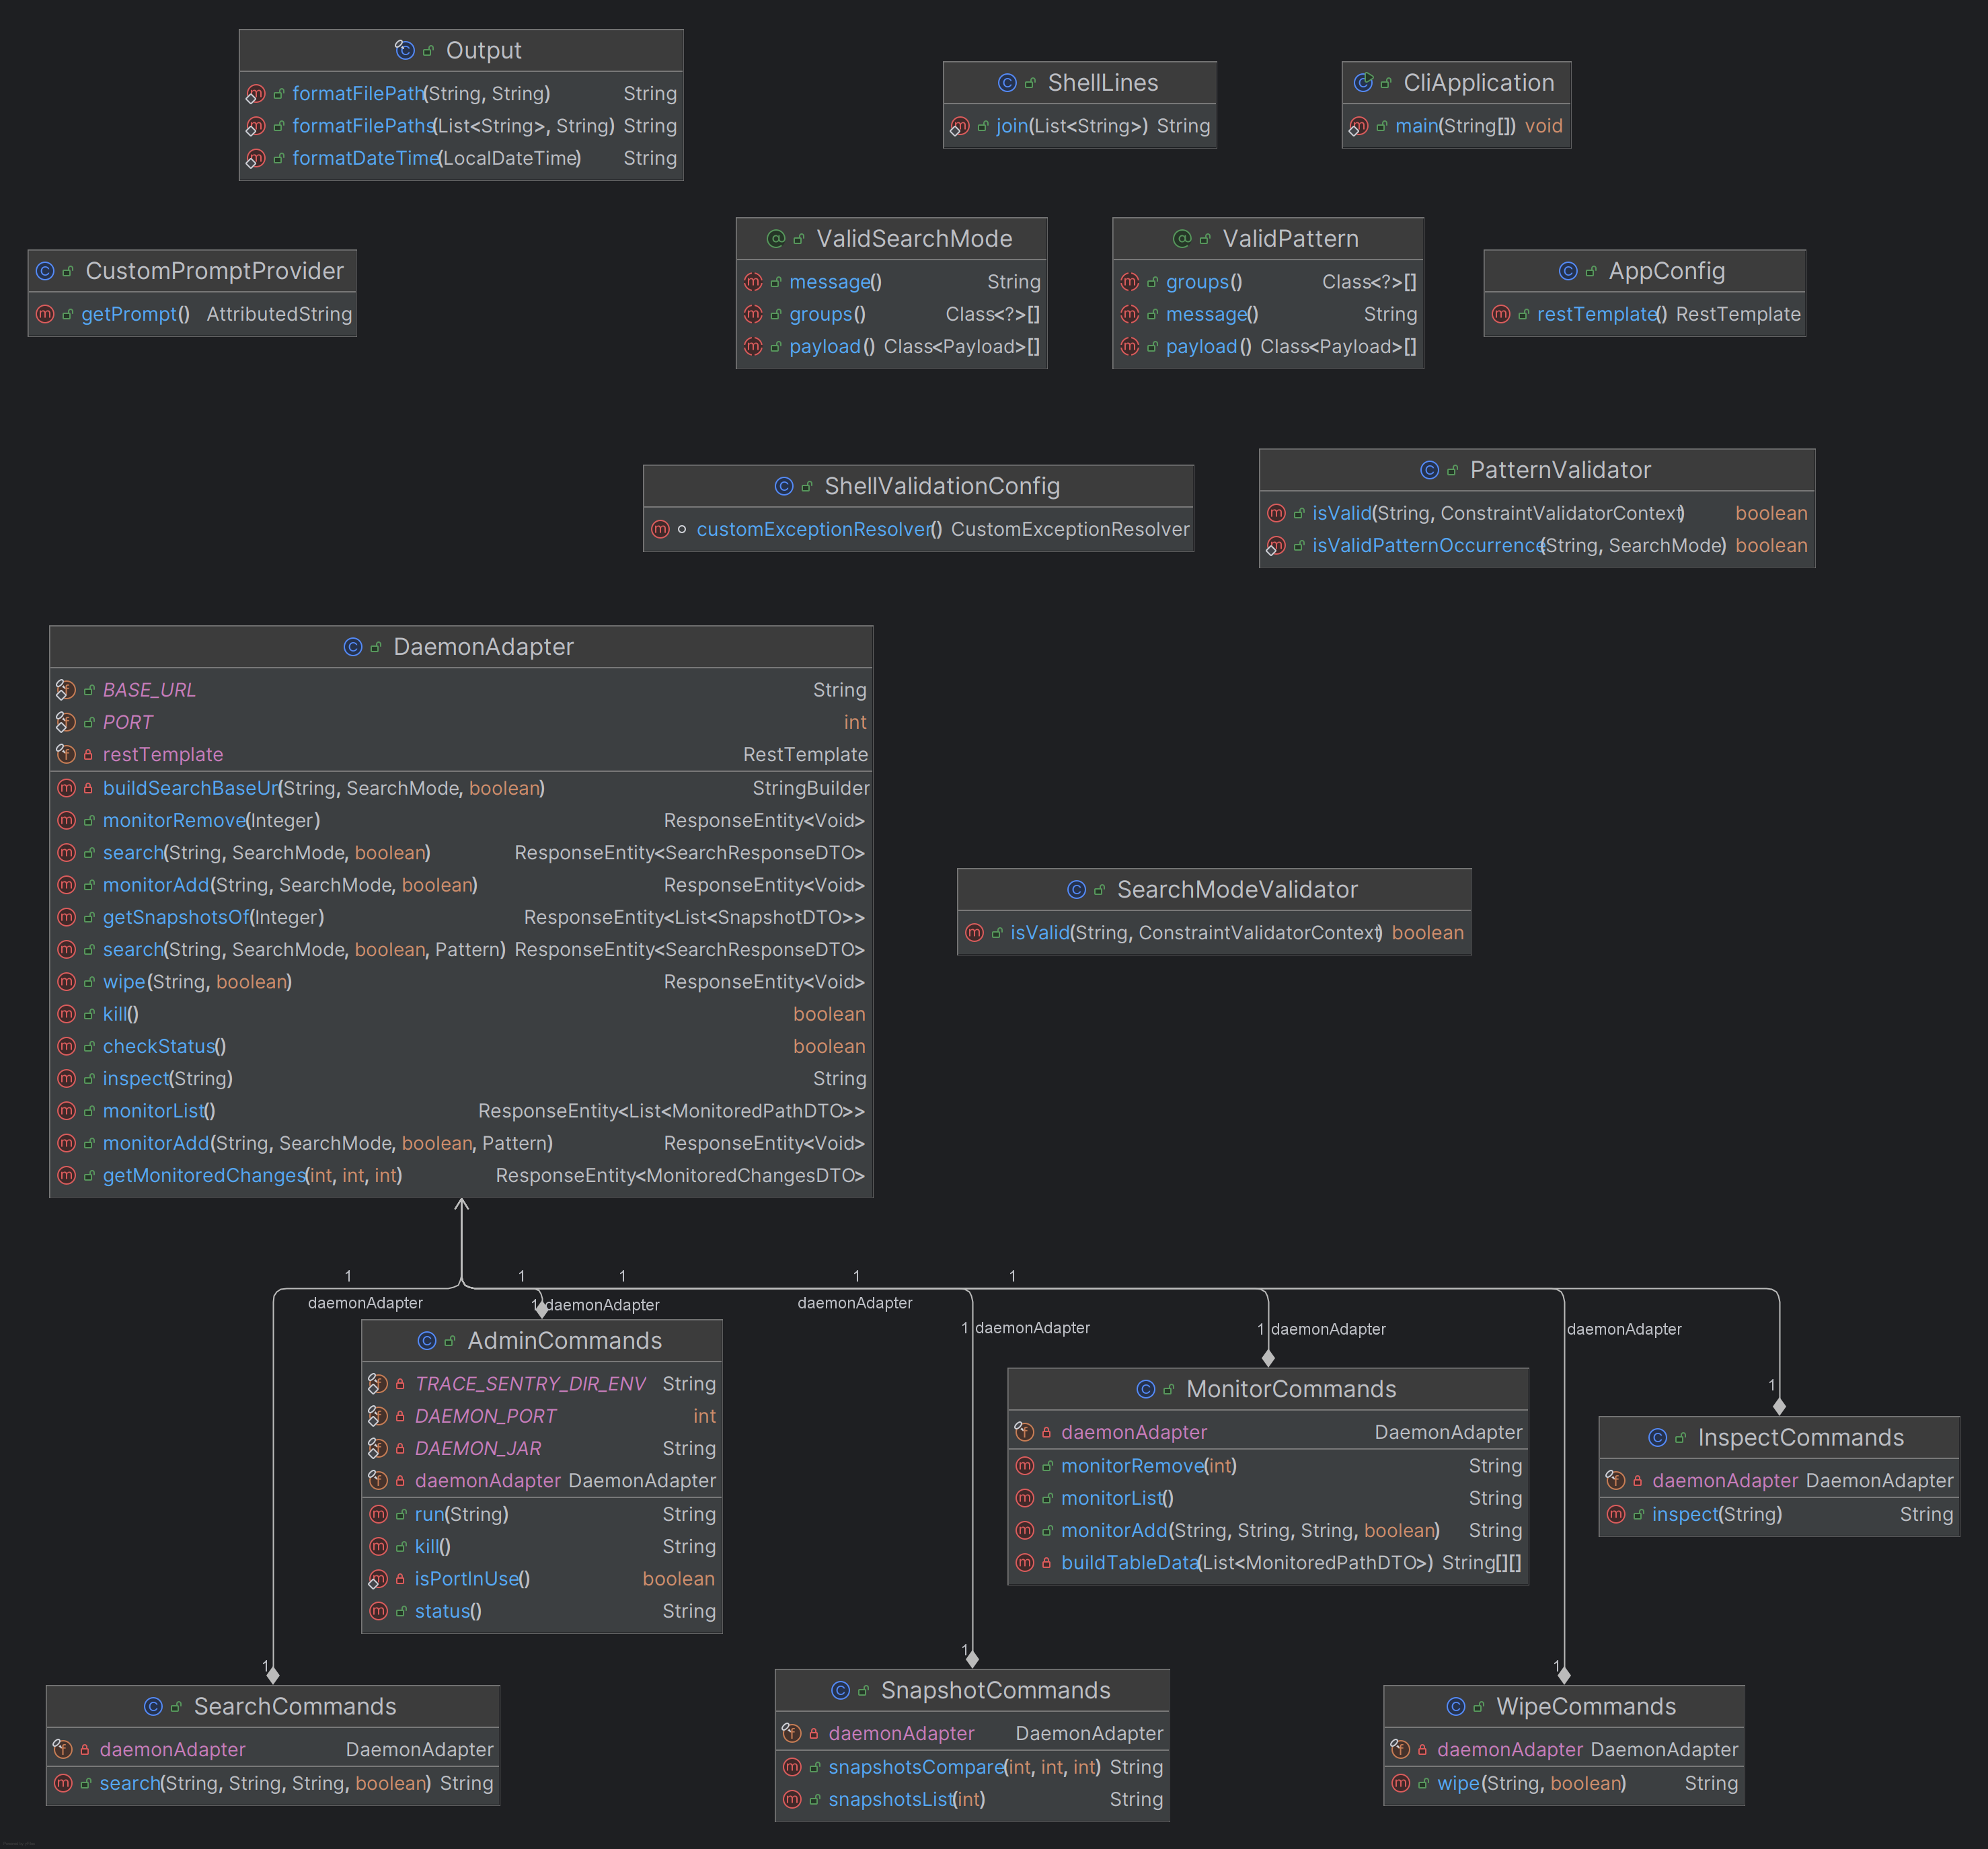
\includepdf[pages=-]{assets/cli_class_diag.png}

    \vspace*{\fill}
    \thispagestyle{empty}
    \titleformat{\section}{\centering\normalfont\Large\bfseries}{\thesection}{1em}{}


    \section{Klassendiagramm Daemon}
    \label{sec:class-diag-daemon}

    \begingroup
    \renewcommand{\thefootnote}{\roman{footnote}}
    \footnotetext[0]{
        \begin{itemize}
            \item Falls das Diagramm nicht optimal dargestellt wird, kann es im Abgabeordner unter folgenden Pfaden gefunden werden:
            \texttt{docs/diagrams/intellij/daemon.uml} (kann nur mit IntelliJ IDEA geöffnet werden) bzw. \texttt{docs/assets/daemon\_class\_diag.png}
            \item Wegen dem Spring IoC Container: nicht alle Beziehungen zwischen Klassen abgebildet.
            \item Diagramm erstellt mit IntelliJ IDEA Ultimate.
        \end{itemize}
    }
    \endgroup

    \vspace*{\fill}
    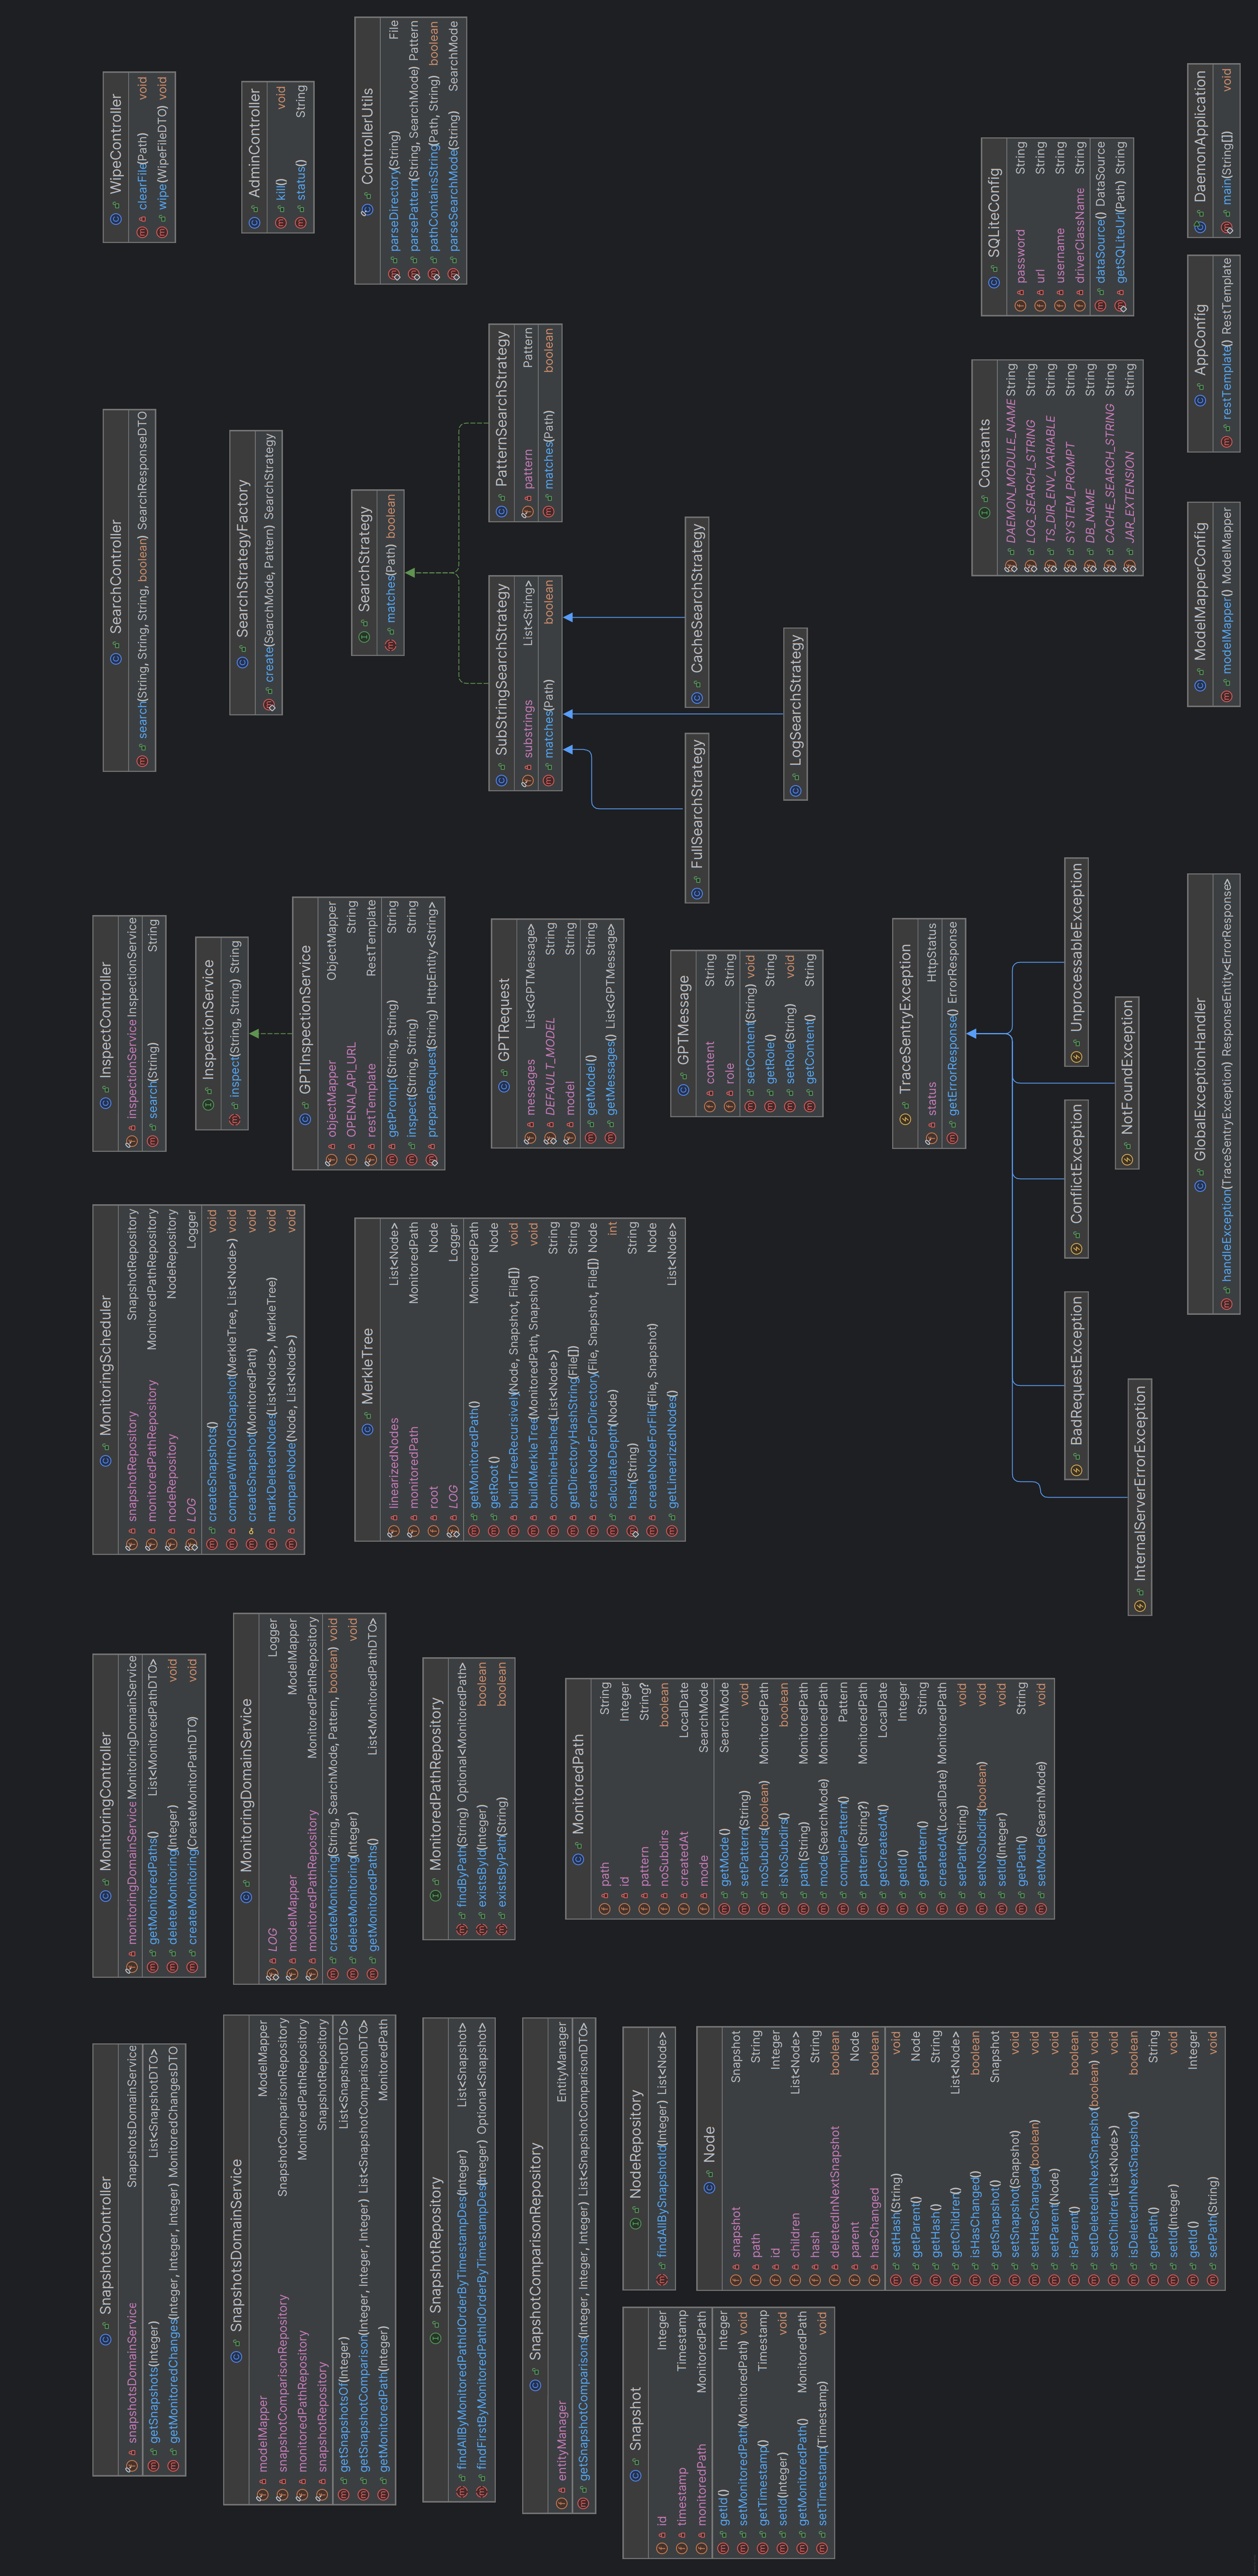
\includepdf[pages=-]{assets/daemon_class_diag.png}

    \vspace*{\fill}
    \thispagestyle{empty}
    \titleformat{\section}{\centering\normalfont\Large\bfseries}{\thesection}{1em}{}


    \section{Klassendiagramm Lib}
    \label{sec:class-diag-lib}

    \begingroup
    \renewcommand{\thefootnote}{\roman{footnote}}
    \footnotetext[0]{
        \begin{itemize}
            \item Falls das Diagramm nicht optimal dargestellt wird, kann es im Abgabeordner unter folgenden Pfaden gefunden werden:
            \texttt{docs/diagrams/intellij/lib.uml} (kann nur mit IntelliJ IDEA geöffnet werden) bzw. \texttt{docs/assets/lib\_class\_diag.png}
            \item Diagramm erstellt mit IntelliJ IDEA Ultimate.
        \end{itemize}
    }
    \endgroup

    \vspace*{\fill}
    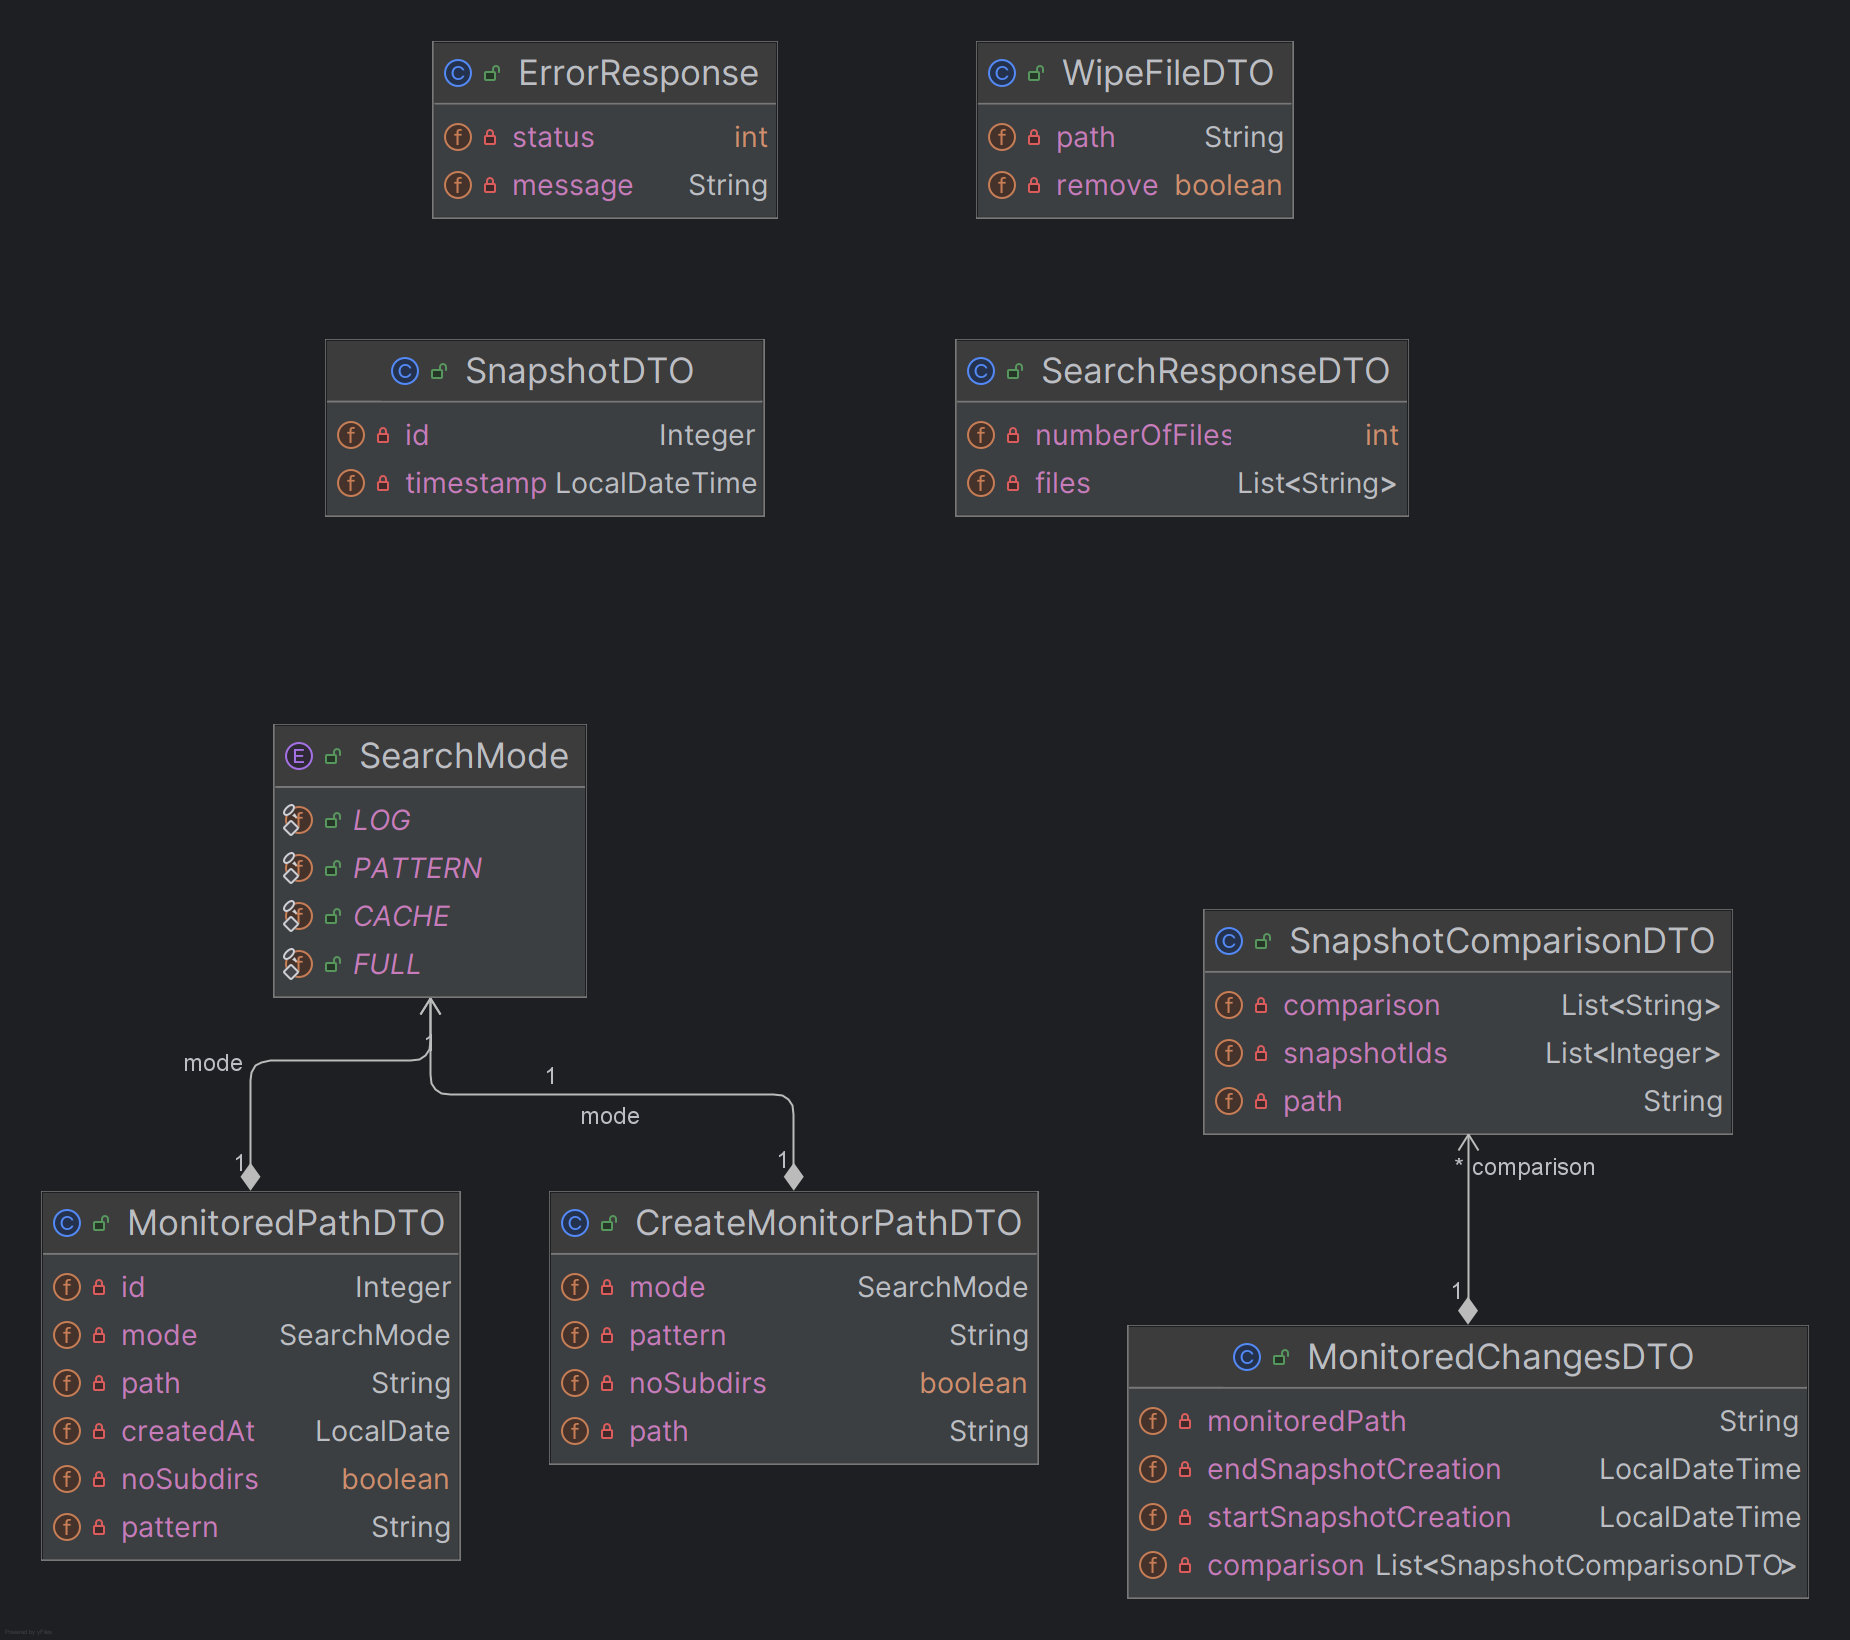
\includepdf[pages=-]{assets/lib_class_diag.png}


    \section{Erklärung zur Urheberschaft}

    Hiermit erklären wir, dass die vorliegende Arbeit selbstständig verfasst wurde und keine anderen als die angegebenen Quellen und Hilfsmittel benutzt wurden.
    \\\\
    Alle Stellen, die wörtlich oder sinngemäß aus anderen Quellen entnommen wurden, sind als solche gekennzeichnet.
    \\\\
    Ich erkläre mich damit einverstanden, dass die vorliegende Arbeit in elektronischer Form mit geeigneter Software überprüft werden darf.

    \begin{flushleft}
        \today
    \end{flushleft}

    \vspace{1cm}

    \begin{center}
        \begin{tabular}{c c c}
            
\includegraphics[width=3cm]{assets/signature1} &
            
\includegraphics[width=3cm]{assets/signature2} &
            
\includegraphics[width=3cm]{assets/signature3} \\
            \rule{3cm}{0.4pt} & \rule{3cm}{0.4pt} & \rule{3cm}{0.4pt} \\
            J. Scherer        & L. Scherer        & L. Ammann
        \end{tabular}
    \end{center}

\end{document}
